\documentclass[12pt]{article}
\usepackage{geometry}
\usepackage{graphicx}
\usepackage{float}
\usepackage{caption}
\usepackage{subcaption}
\usepackage{booktabs}
\usepackage{amsmath}
\usepackage{hyperref}
\usepackage{siunitx}
\usepackage{tocloft}
\renewcommand{\cftsecfont}{\normalsize} % font size for sections
\renewcommand{\cftsubsecfont}{\small}   % smaller font for subsections
\renewcommand{\cftsecpagefont}{\normalsize} 
\renewcommand{\cftsubsecpagefont}{\small}
\renewcommand{\cftbeforesecskip}{0pt}   % remove extra vertical space
\renewcommand{\cftbeforesubsecskip}{0pt}
\setlength{\cftsecindent}{0pt}
\setlength{\cftsubsecindent}{15pt}

\geometry{margin=1in}
\graphicspath{{figures/}}

\begin{document}

% ------------------ COVER PAGE ------------------
\begin{titlepage}
    \centering
    \vspace*{0.1cm}
    {\huge LUT Characterization \\[0.5em]}
    {\large Fall 2025 \\[2em]}

    \includegraphics[width=\linewidth]{LUT_sch.png}\\[2em]

    \textbf{Authors:} Krishna Karthikeya Chemudupati, Taarana Jammula \\[2em]

    \vfill
\end{titlepage}

% ------------------ TABLE OF CONTENTS ------------------
\tableofcontents
\newpage

% ------------------ SECTION 1 ------------------
\section{Baseline Design Schematics}

\subsection{Minimum Size Inverter}

\subsubsection*{Schematic}

\begin{figure}[H]
    \centering
    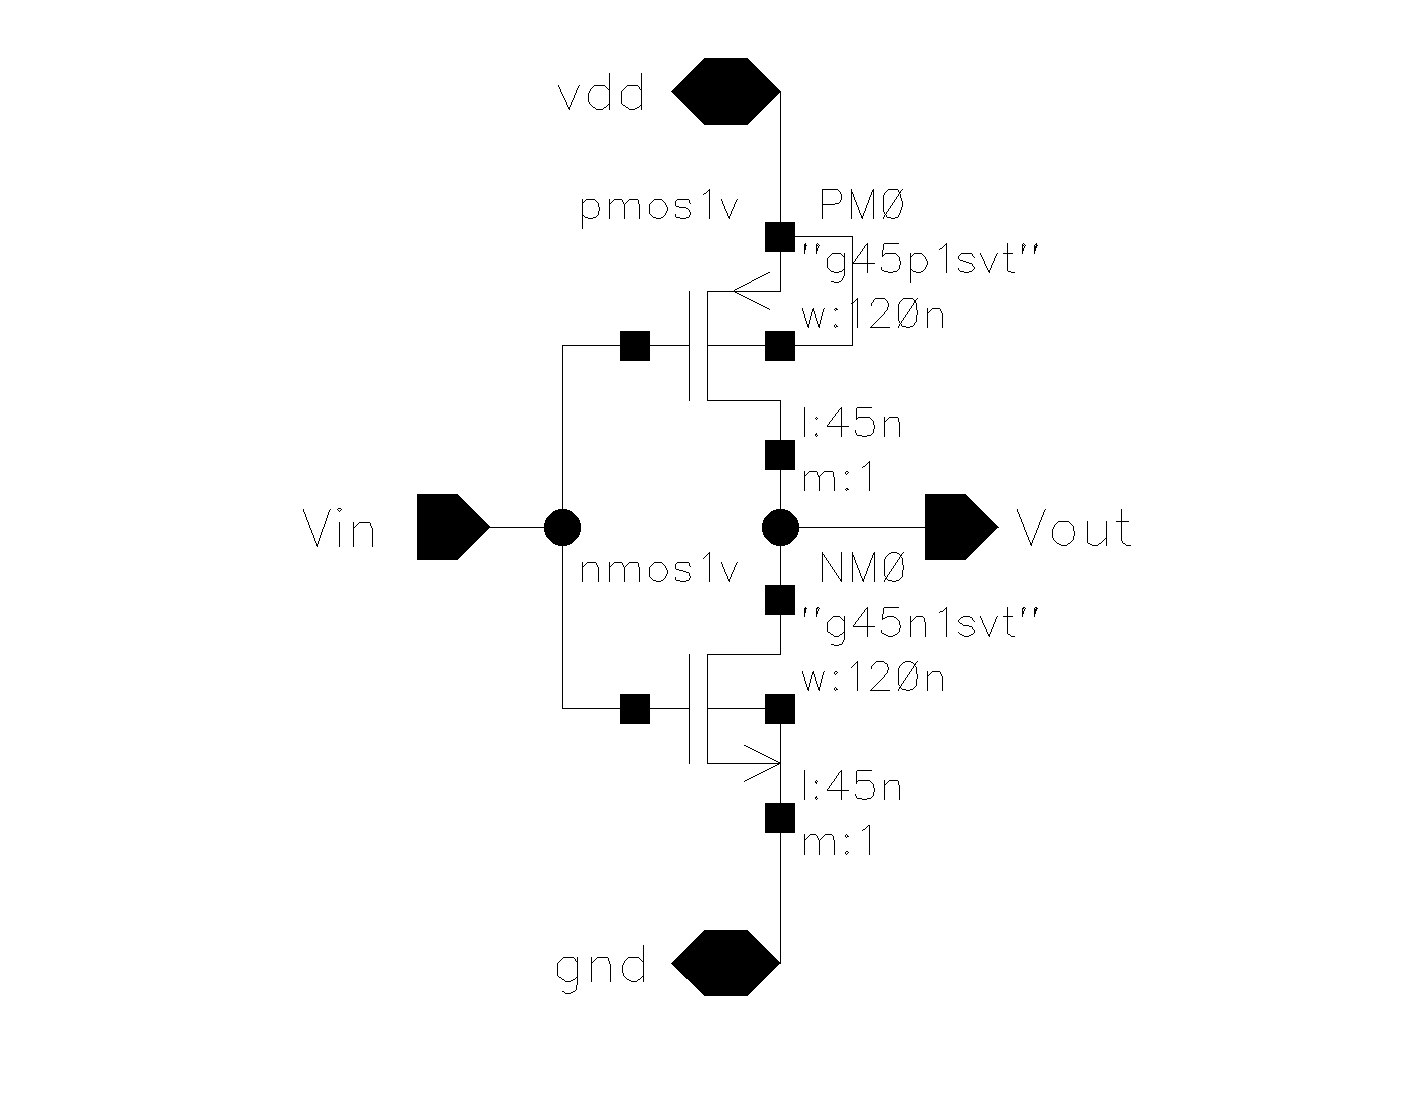
\includegraphics[width=0.5\linewidth]{writeup//figures/inv_sch.png}
    \caption{Enter Caption}
\end{figure}

\subsubsection*{Symbol}

\begin{figure}[H]
    \centering
    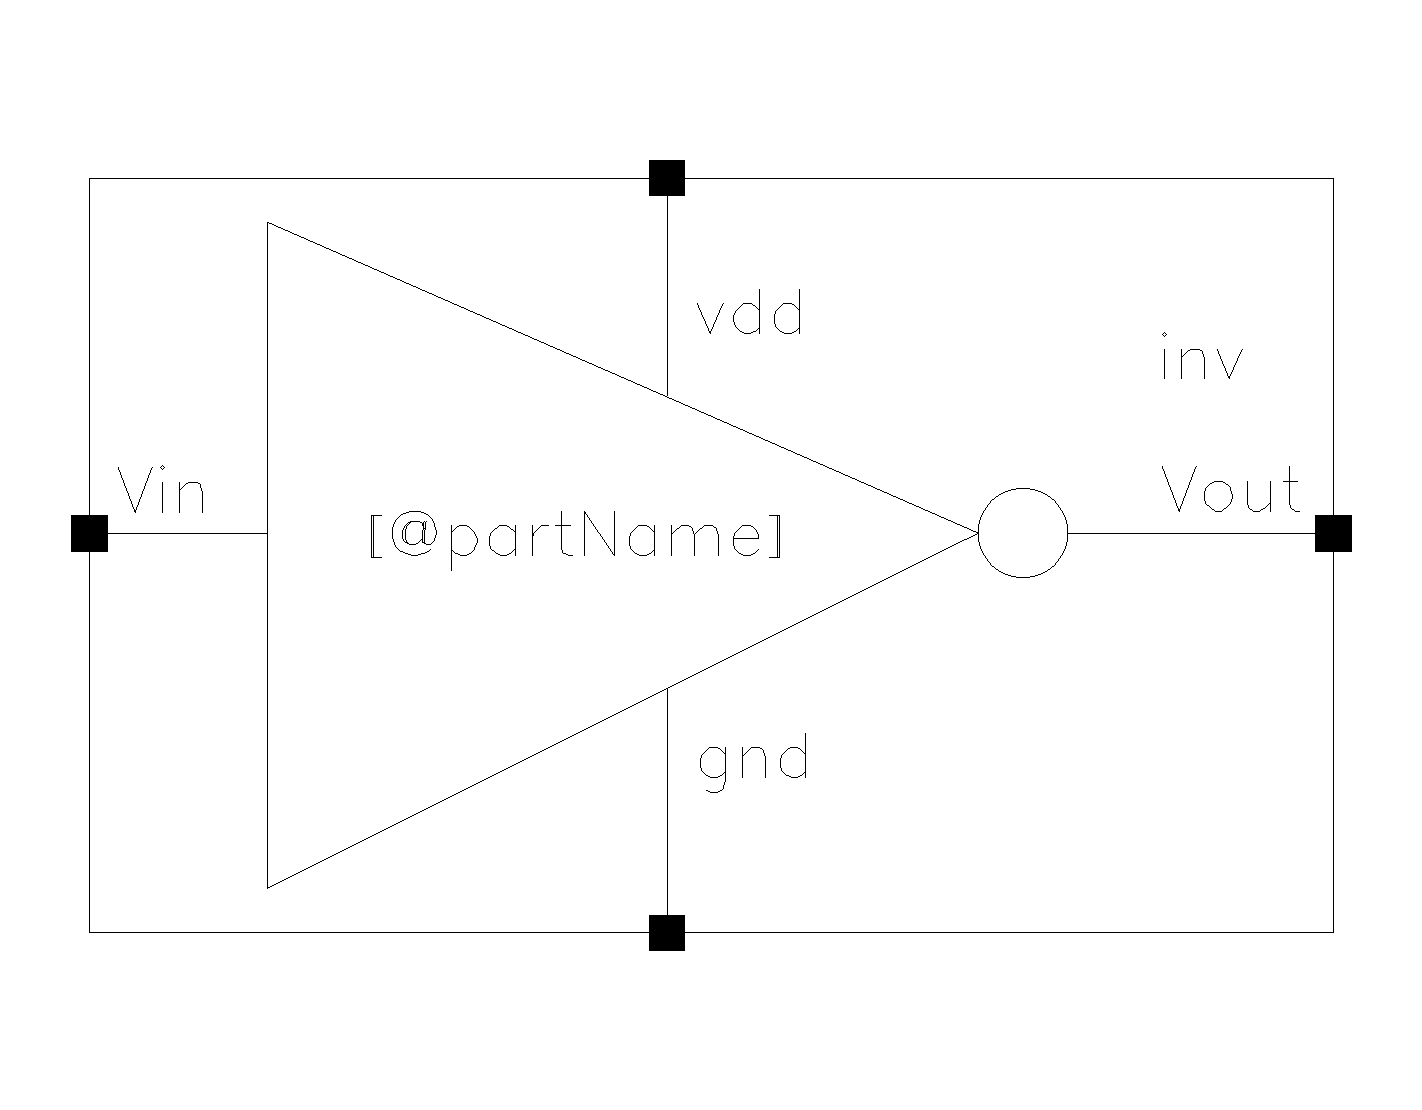
\includegraphics[width=0.5\linewidth]{writeup//figures/inv_sym.png}
    \caption{Enter Caption}
\end{figure}

\newpage

\subsection{2:1 MUX Design}

\subsubsection*{Schematic}

\begin{figure}[H]
    \centering
    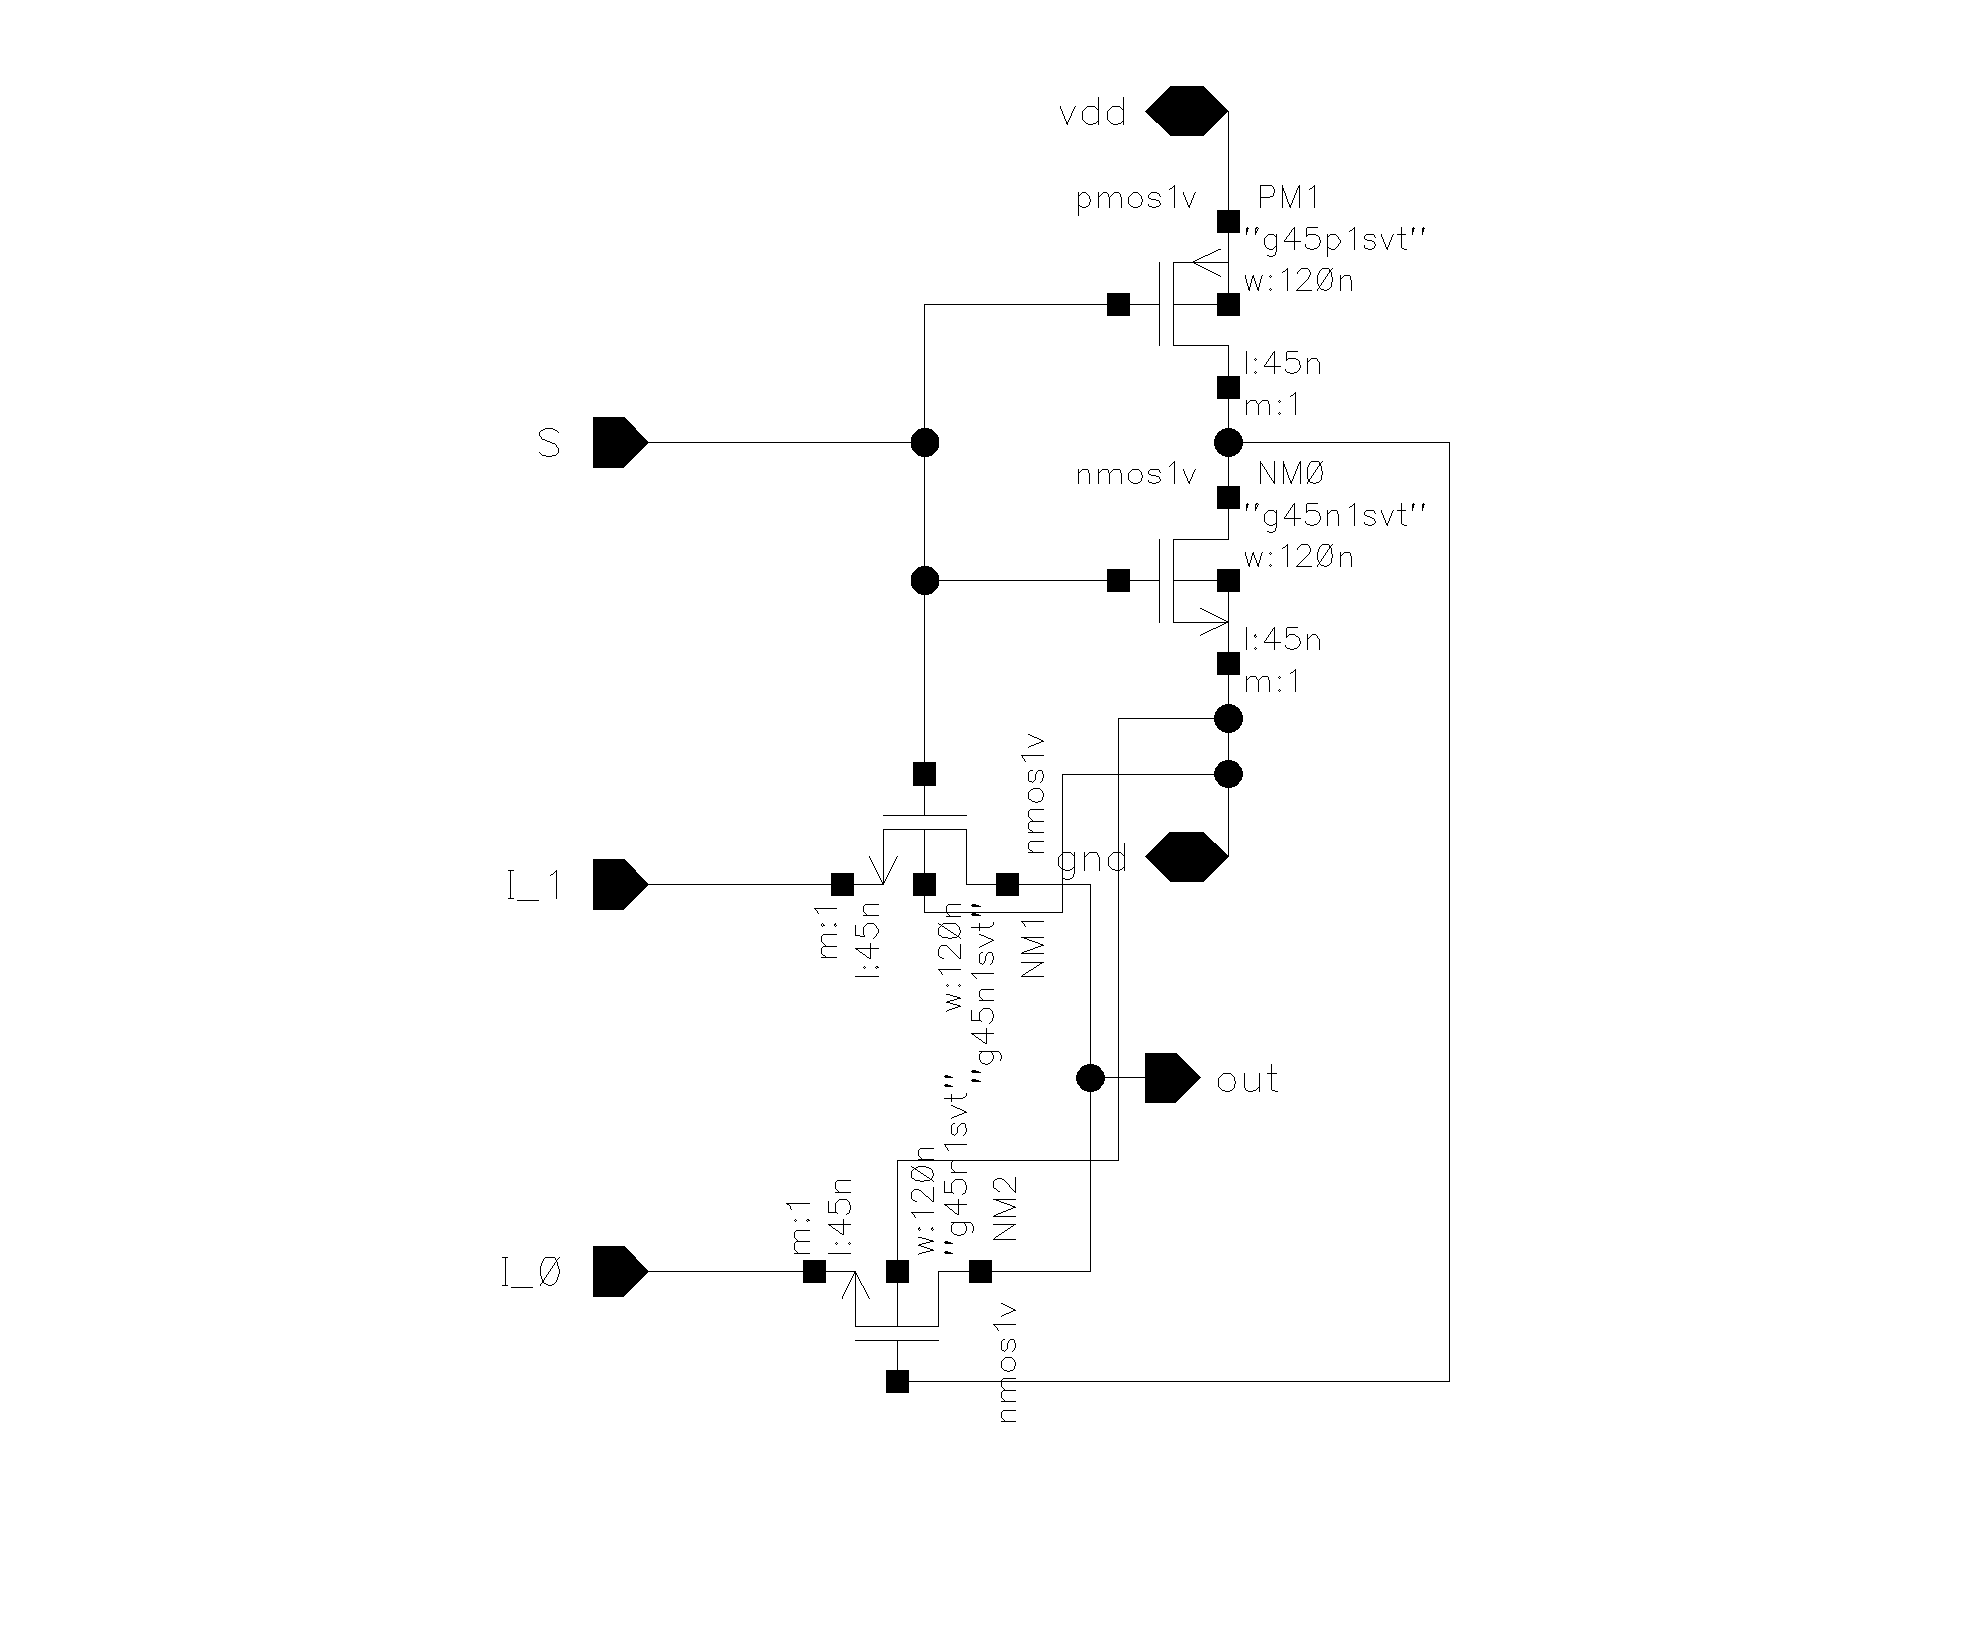
\includegraphics[width=0.5\linewidth]{writeup//figures/MUX_sch.png}
    \caption{Enter Caption}
\end{figure}

\subsubsection*{Symbol}

\begin{figure}[H]
    \centering
    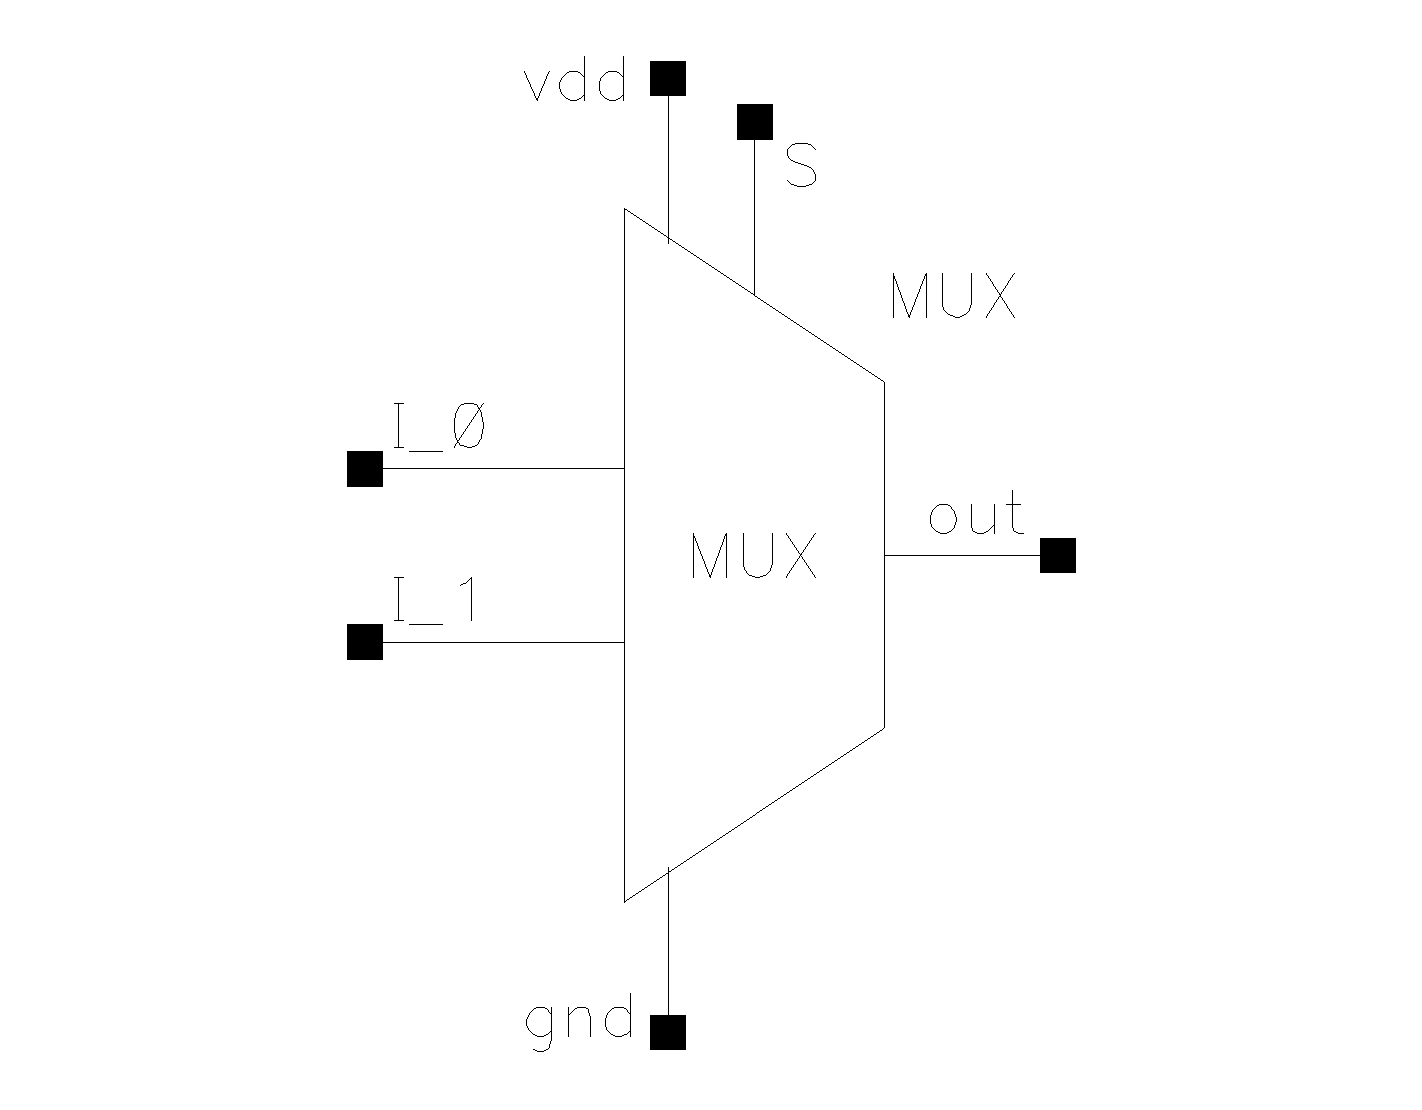
\includegraphics[width=0.5\linewidth]{writeup//figures/MUX_sym.png}
    \caption{Enter Caption}
\end{figure}

\newpage

\subsection{16:1 LUT Design}
\subsubsection*{Schematic}
\begin{figure}[H]
    \centering
    \includegraphics[width=0.5\linewidth]{writeup//figures/LUT_sch.png}
    \caption{Enter Caption}
\end{figure}

\subsubsection*{Symbol}
\begin{figure}[H]
    \centering
    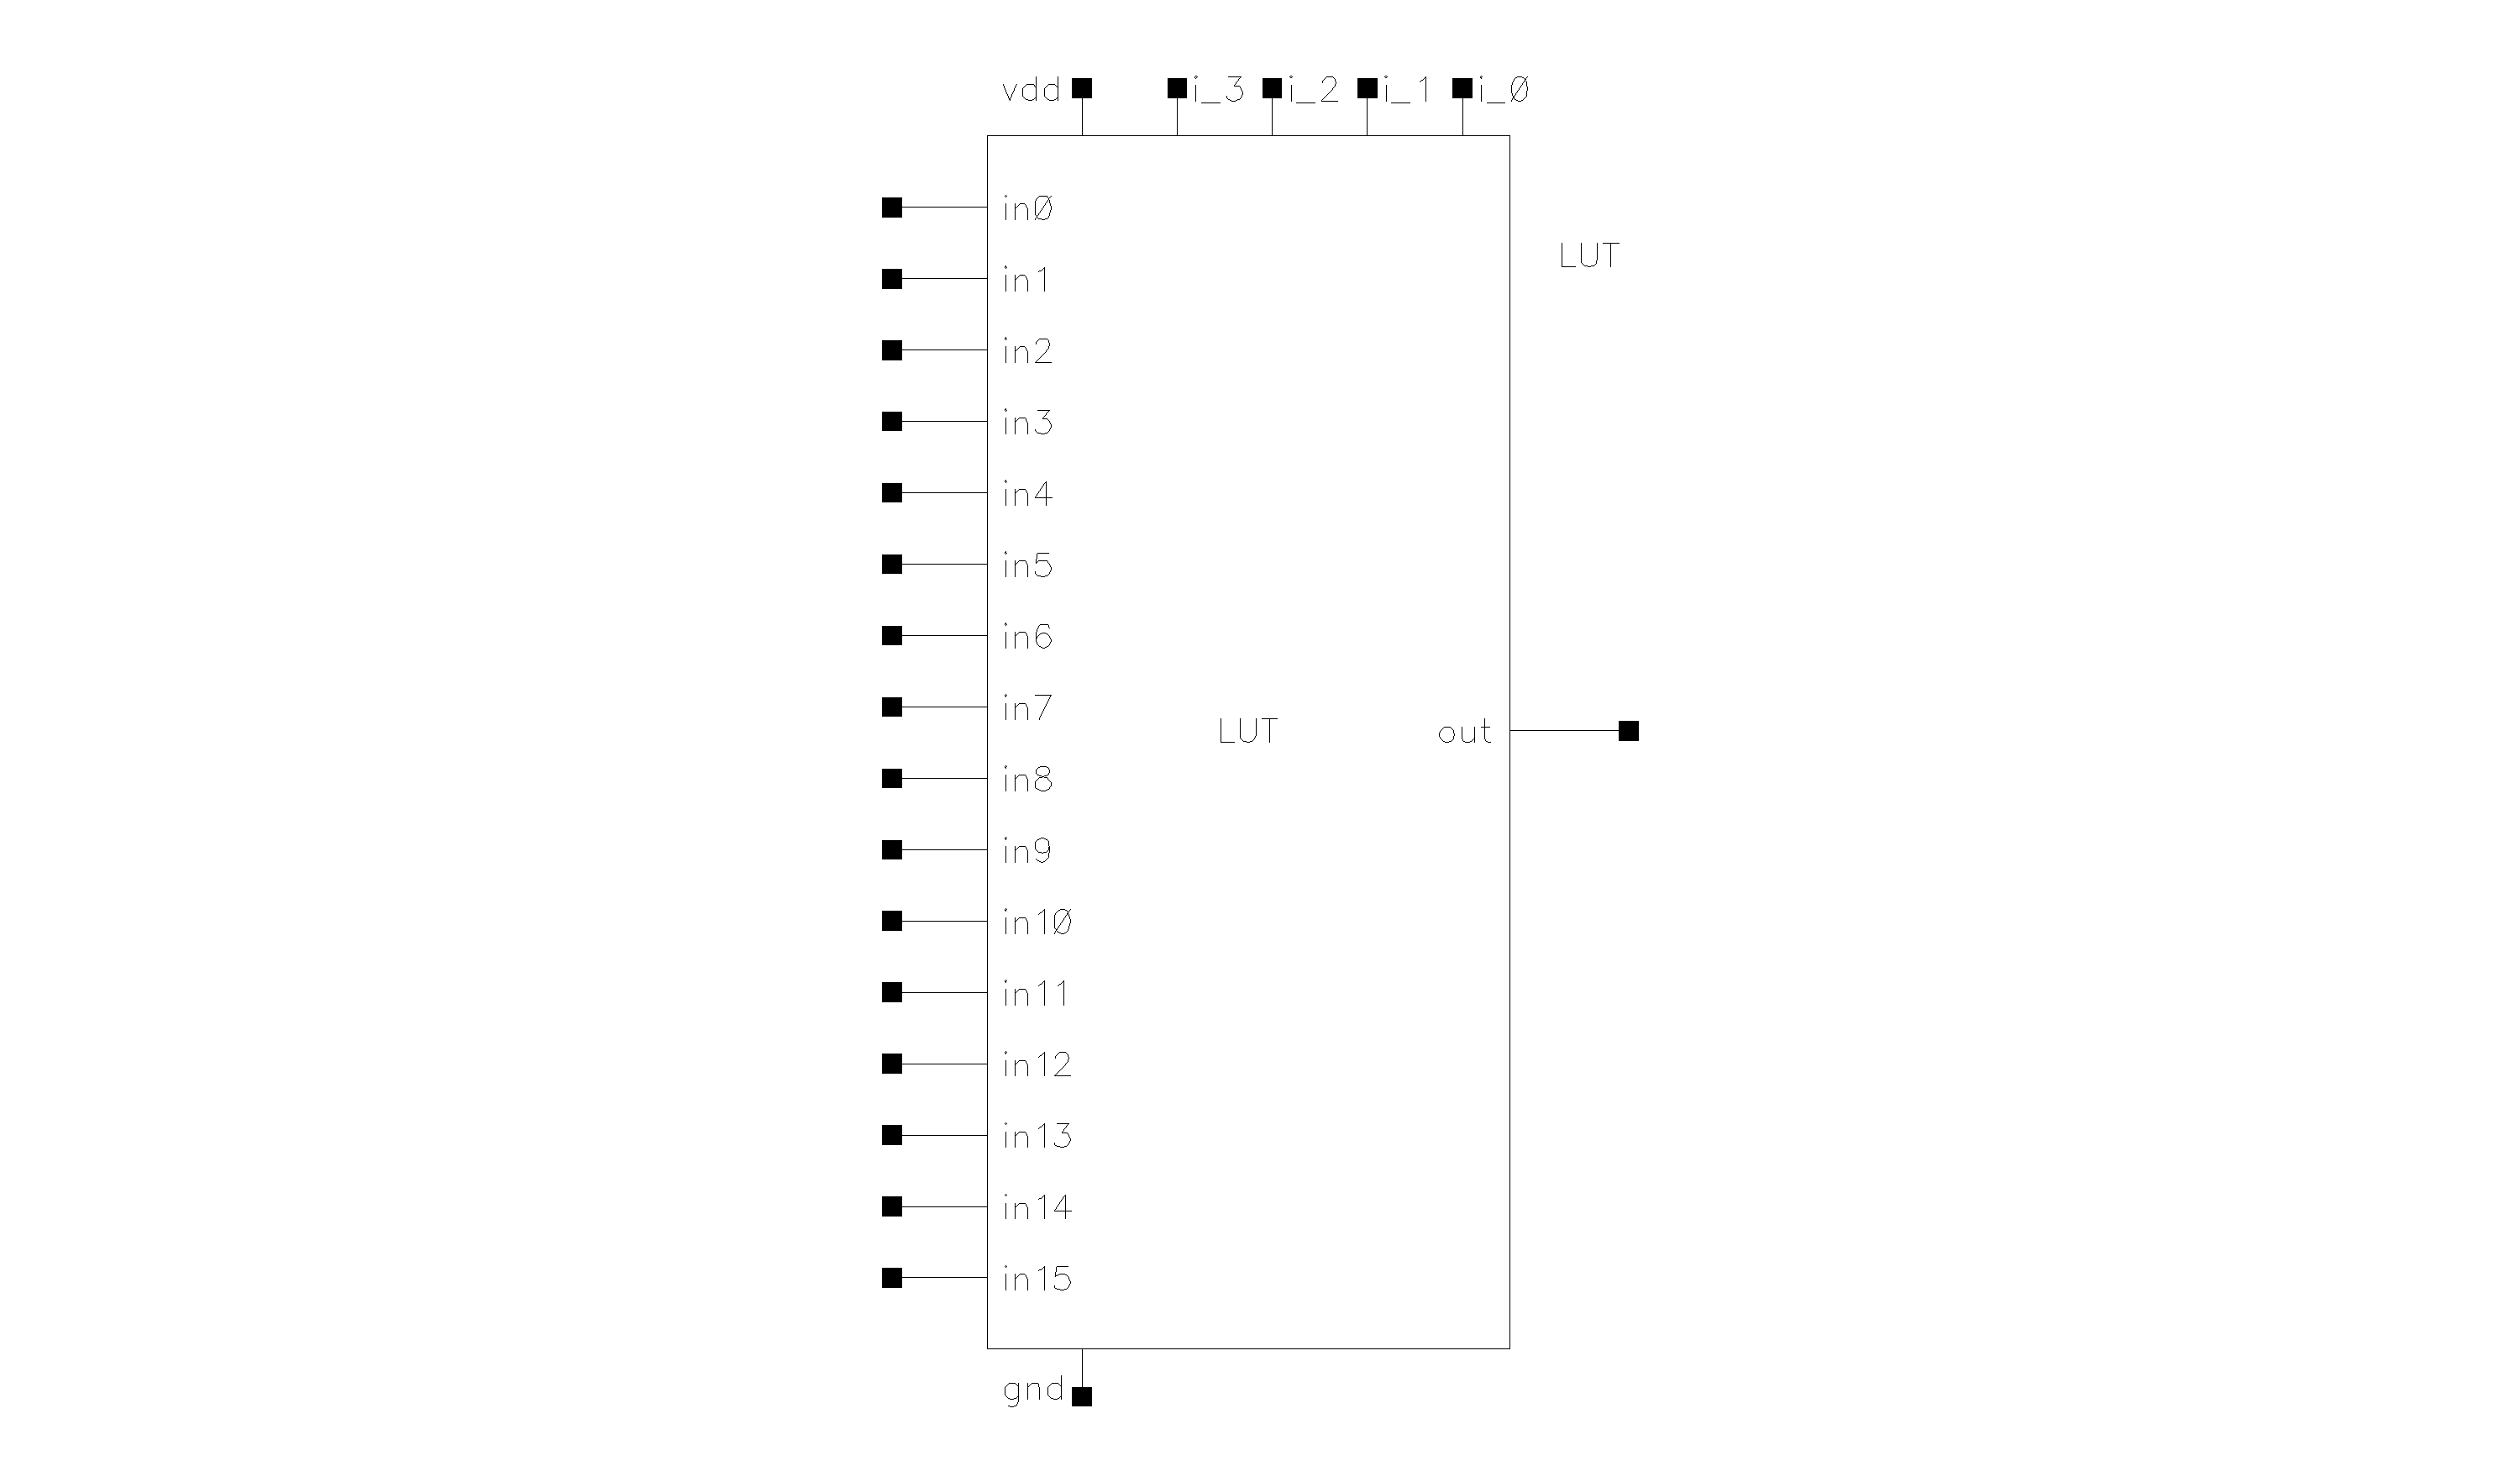
\includegraphics[width=0.5\linewidth]{writeup//figures/LUT_sym.png}
    \caption{Enter Caption}
\end{figure}

\newpage

% ------------------ SECTION 2 ------------------
\section{Baseline Design Validation and Logical Test}
\subsection{Test Schematic and Case}
\subsubsection*{Test Schematics}

\begin{figure}[H]
    \centering
    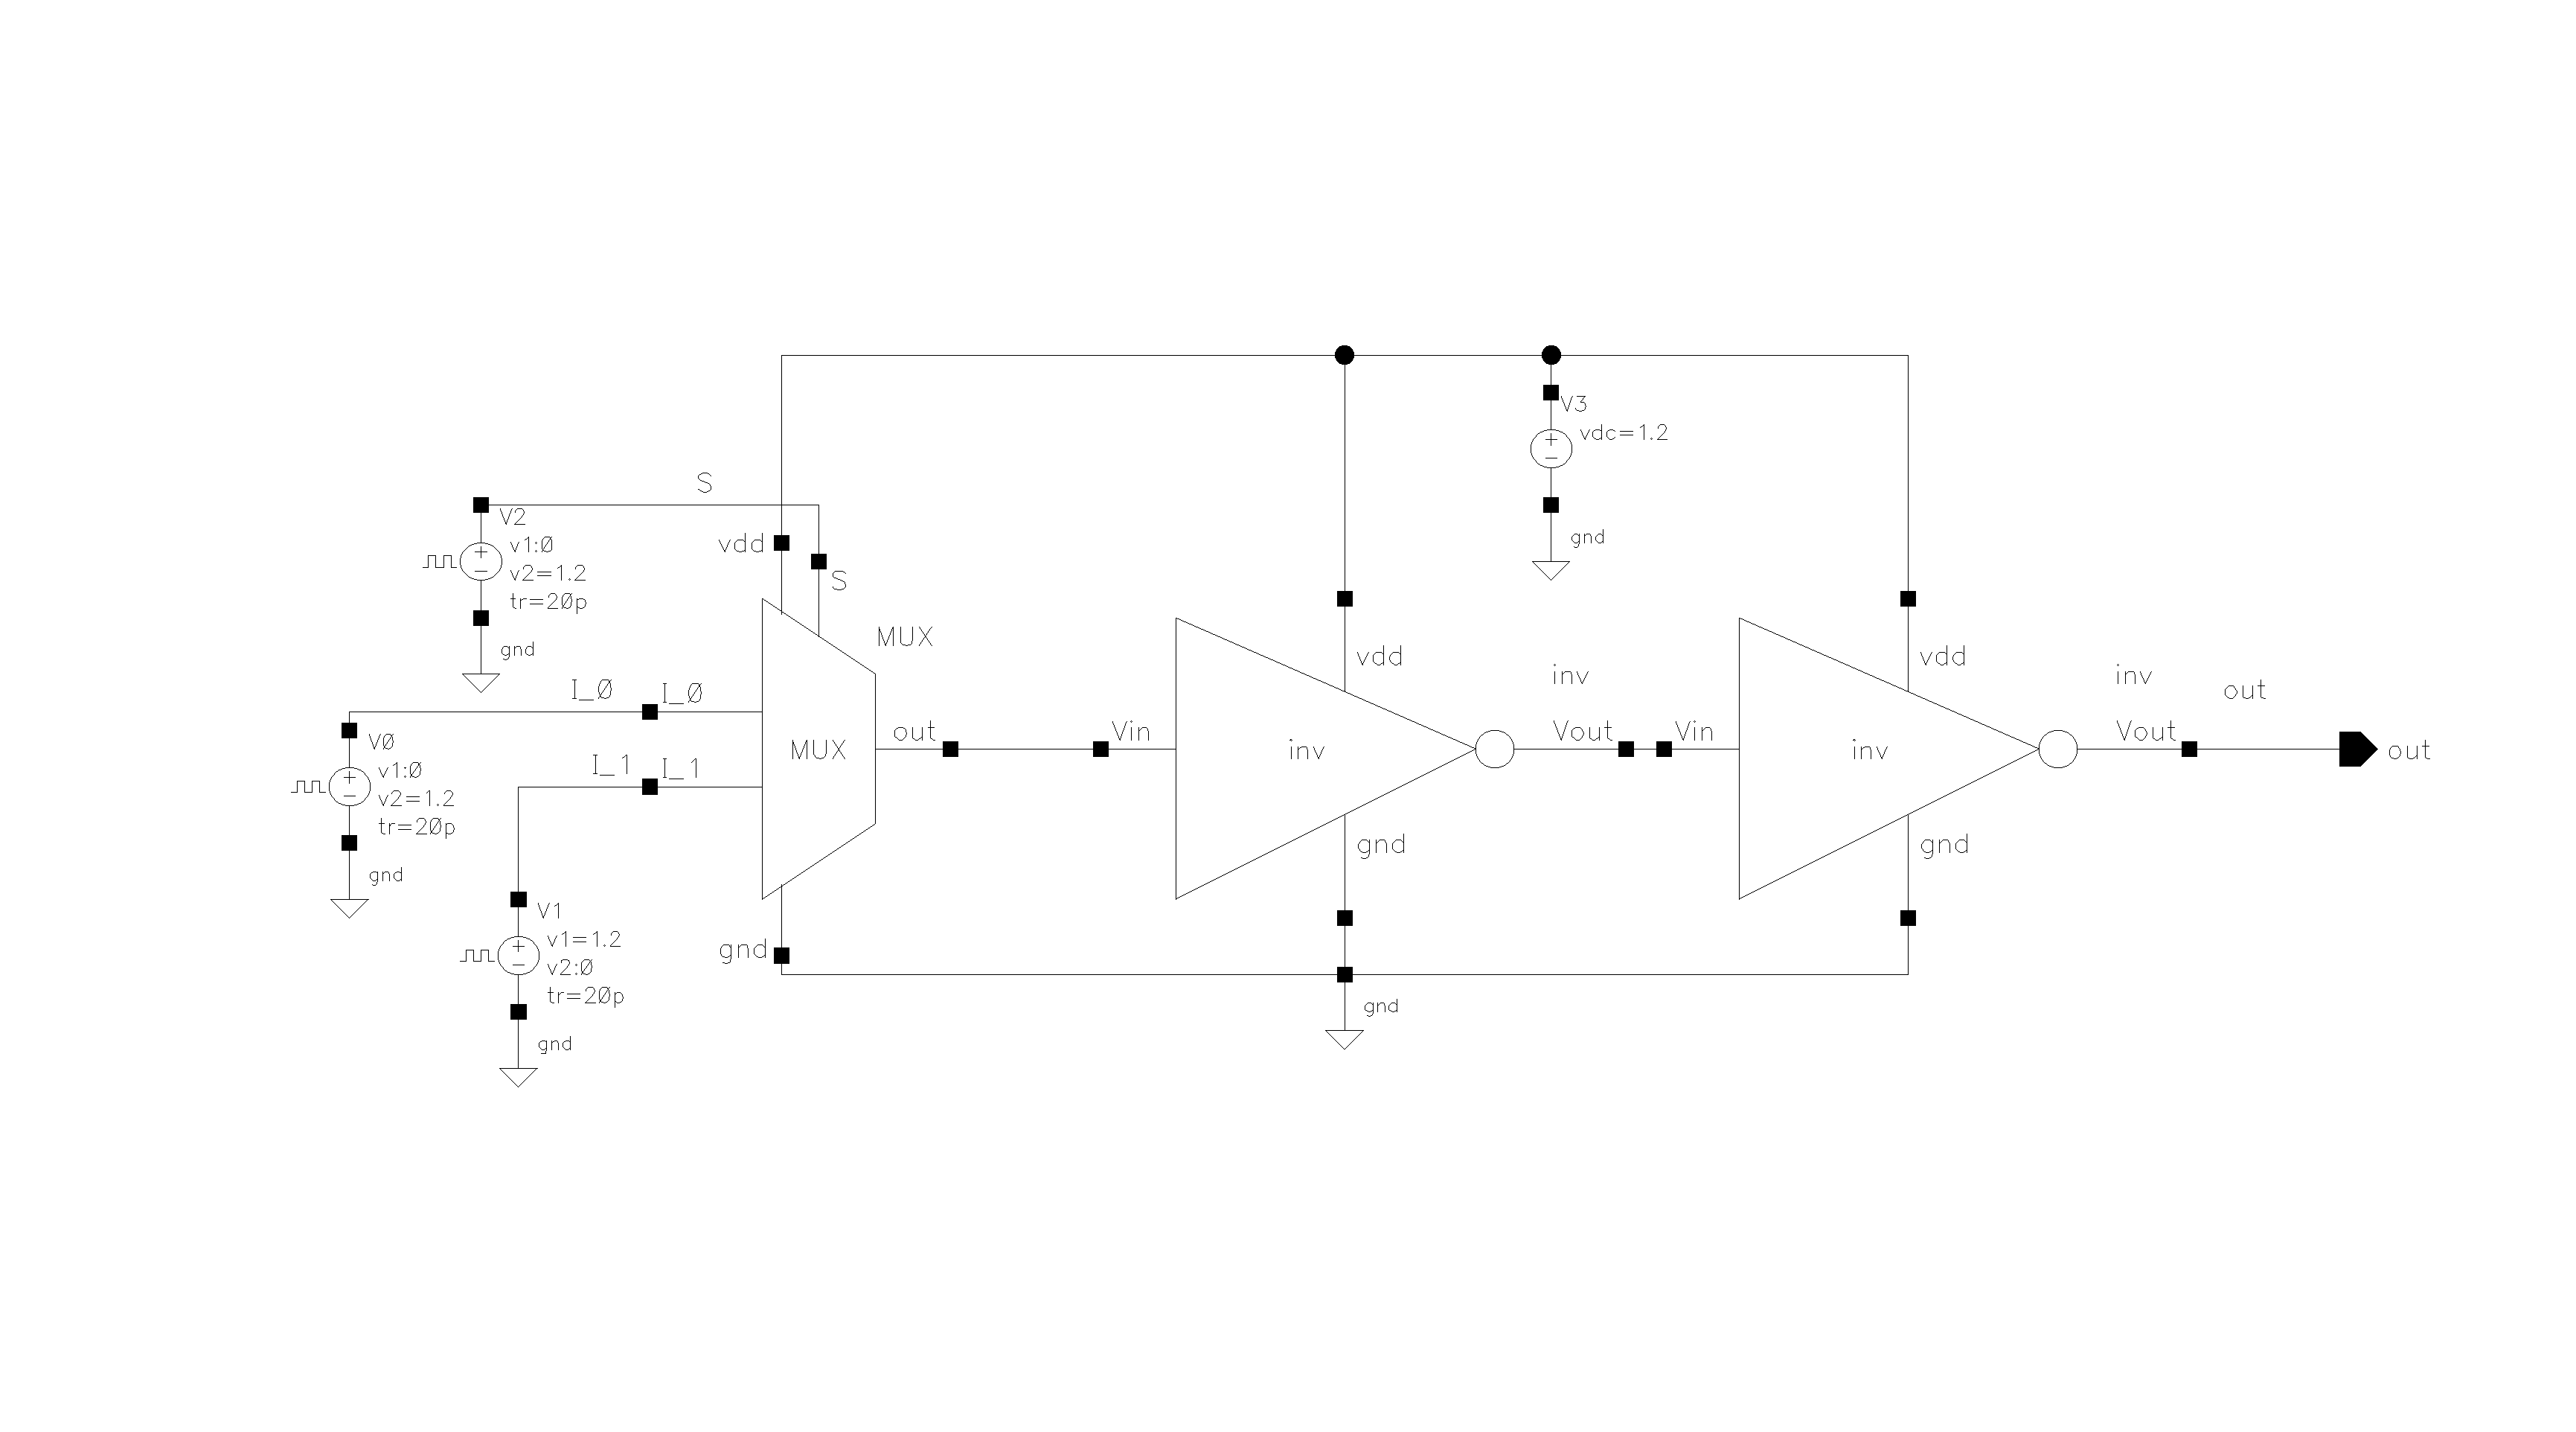
\includegraphics[width=0.5\linewidth]{writeup//figures/muxsubtestschem.png}
    \caption{Enter Caption}
\end{figure}

\begin{figure}[H]
    \centering
    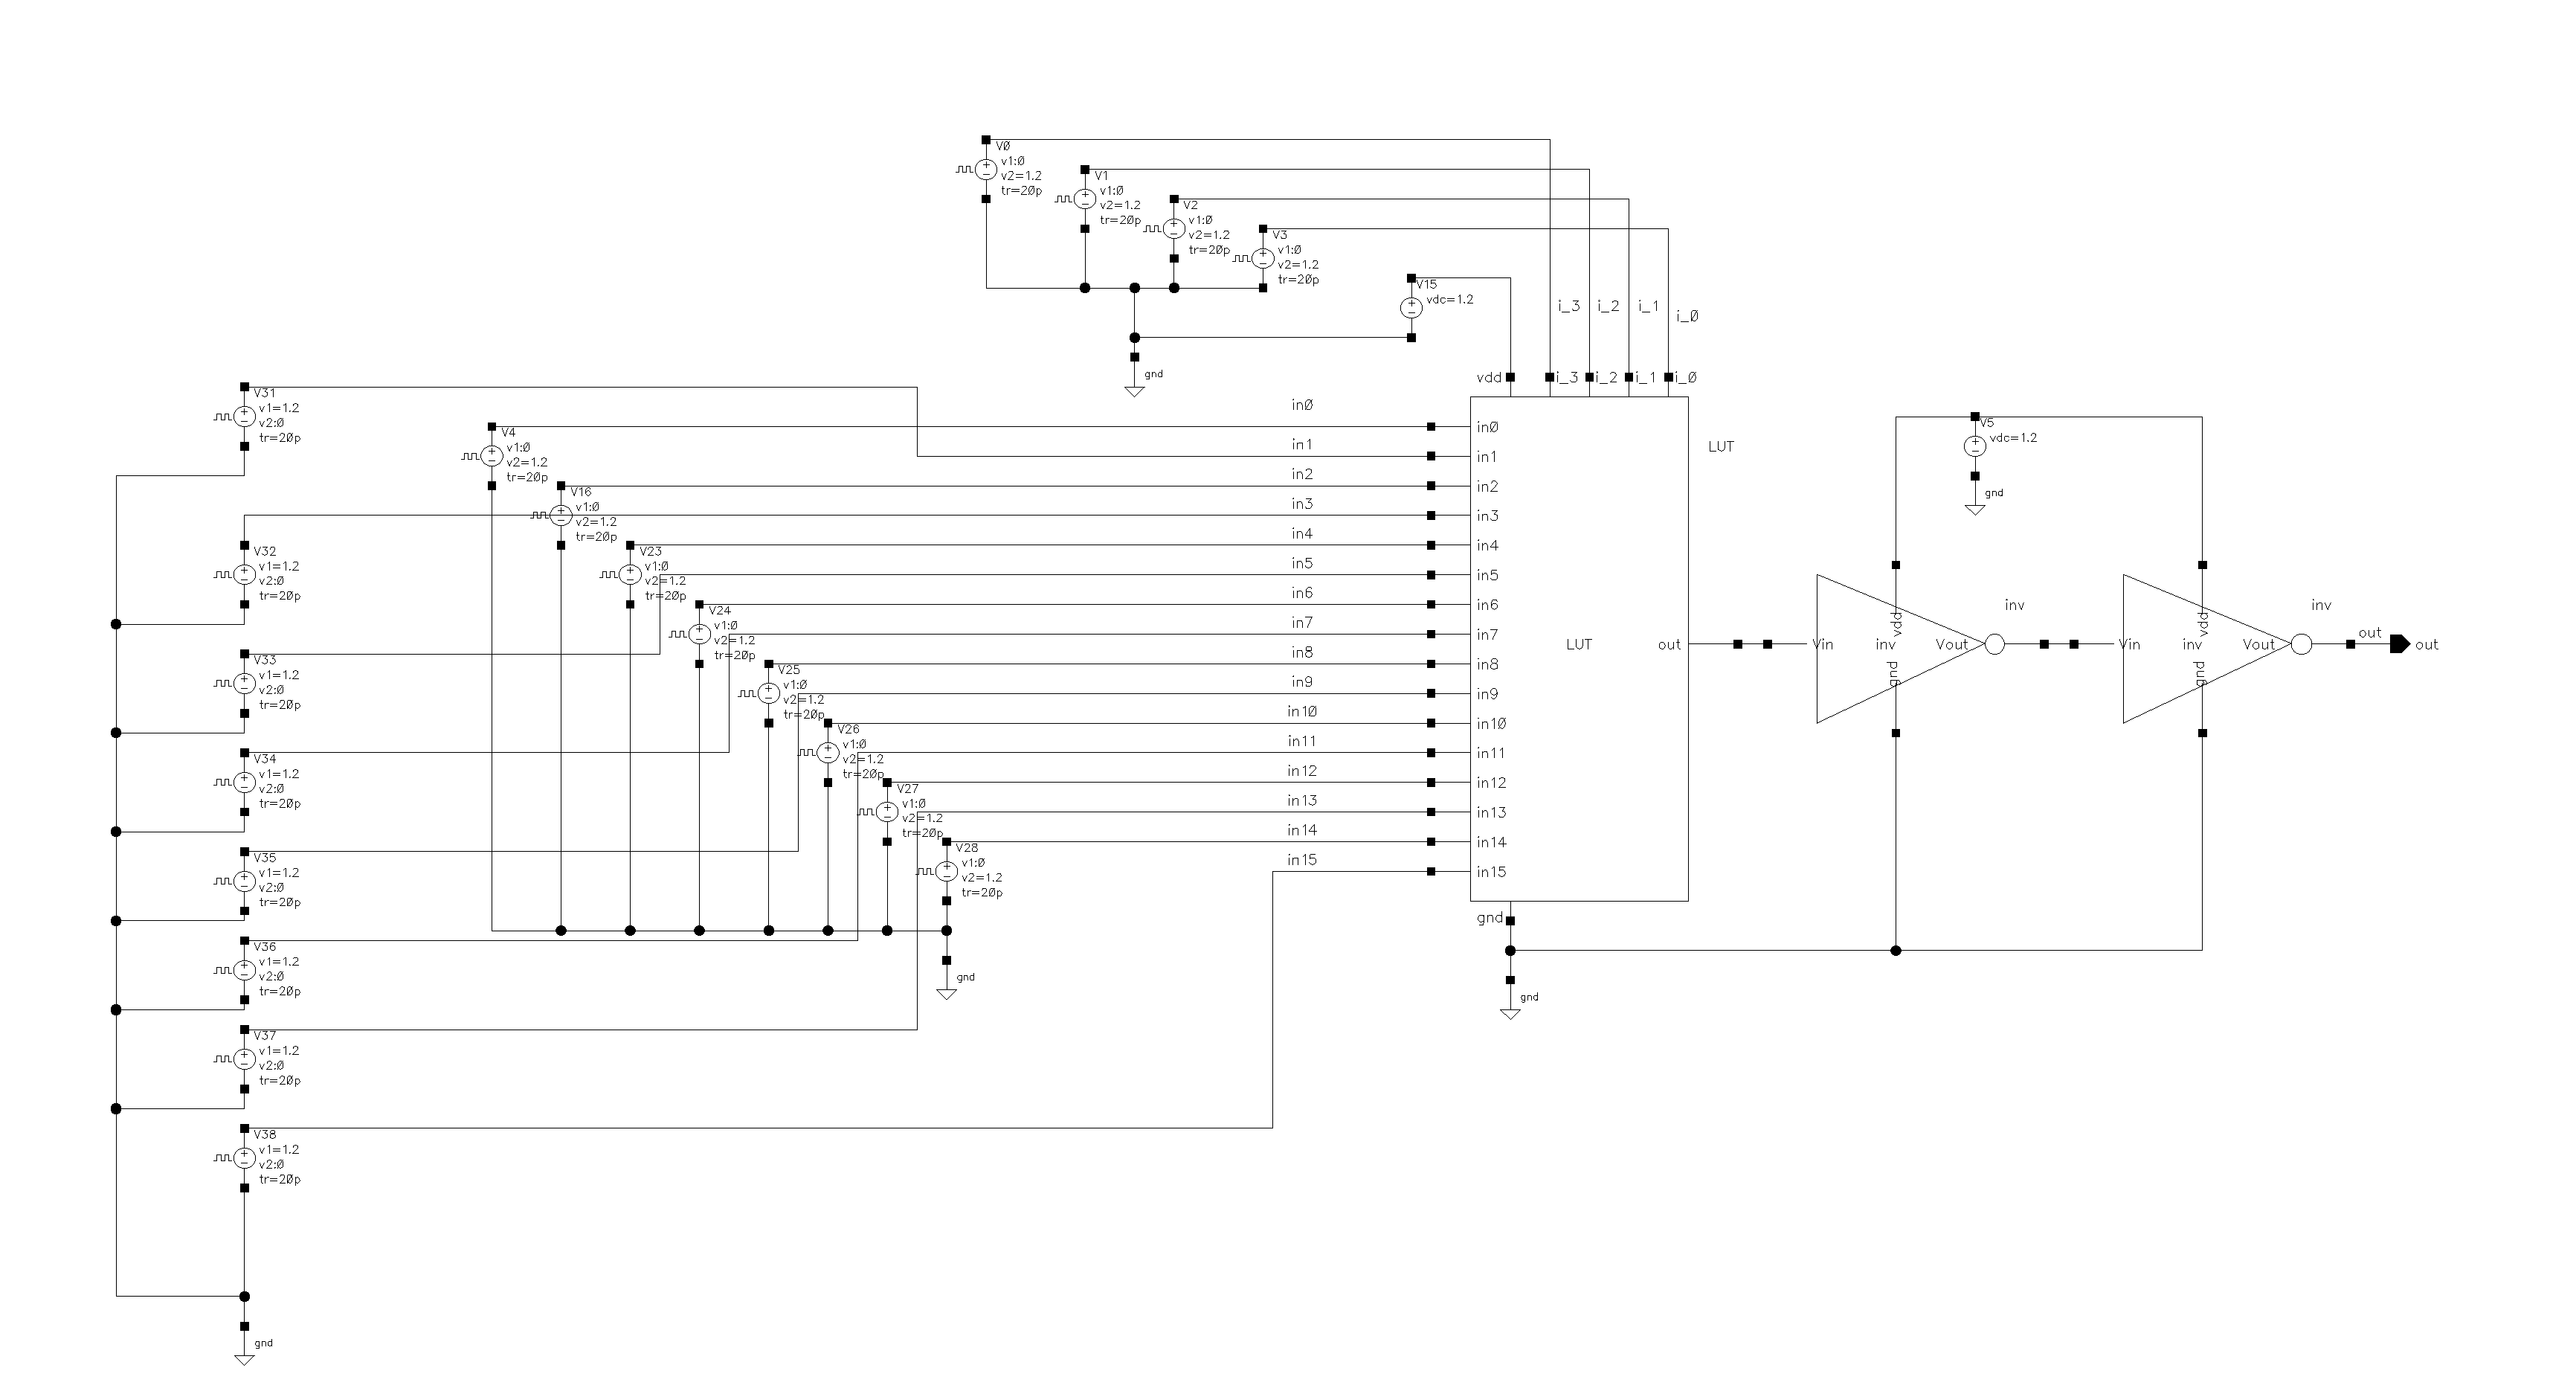
\includegraphics[width=0.5\linewidth]{writeup//figures/luttestschem.png}
    \caption{Enter Caption}
\end{figure}

\subsubsection*{Cases}
For the 2:1 MUX validation, the input signals were configured to ensure that both selection paths could be distinctly verified. The data input \( I_1 \) was driven with a square wave transitioning from low to high, while \( I_0 \) was driven with an inverse square wave (high to low). The select line \( S \) was given a signal with \textbf{double the period} of the data inputs to allow for multiple transitions of \( I_0 \) and \( I_1 \) within each select cycle. 
This setup ensures that during each half-period of \( S \), both data inputs experience a full logic transition, allowing the output to alternate between following \( I_0 \) and \( I_1 \) depending on the state of \( S \). 
By measuring the output \( V_{\text{out}} \) and observing that it follows \( I_1 \) when \( S=1 \) and \( I_0 \) when \( S=0 \), the expected multiplexer behavior was confirmed. The corresponding transient waveform verified this switching behavior with minimal propagation delay between the input and output transitions.

For the 16:1 LUT validation, a counter-type input pattern was applied to systematically generate all \( 2^4 = 16 \) address combinations. 
Each address line was assigned a different pulse period to form a binary counting sequence: \( I_3 \) with a 2\,ns period, \( I_2 \) with 4\,ns, \( I_1 \) with 8\,ns, and \( I_0 \) with 16\,ns. This timing scheme ensures that over one full 16-state cycle, every unique combination from \( 0000 \) to \( 1111 \) is applied to the address inputs. All sixteen data inputs (\( \text{IN}_0 \) through \( \text{IN}_{15} \)) were driven with identical 8\,ns square waves to maintain consistent signal activity. 
As the address counter advanced, the output \( V_{\text{out}} \) was observed to follow the corresponding data input for each address state, verifying correct selection logic and full LUT functionality.

\subsection{Validation}
\subsubsection*{2:1 MUX Subcircuit Validation}
\begin{figure}[H]
    \centering
    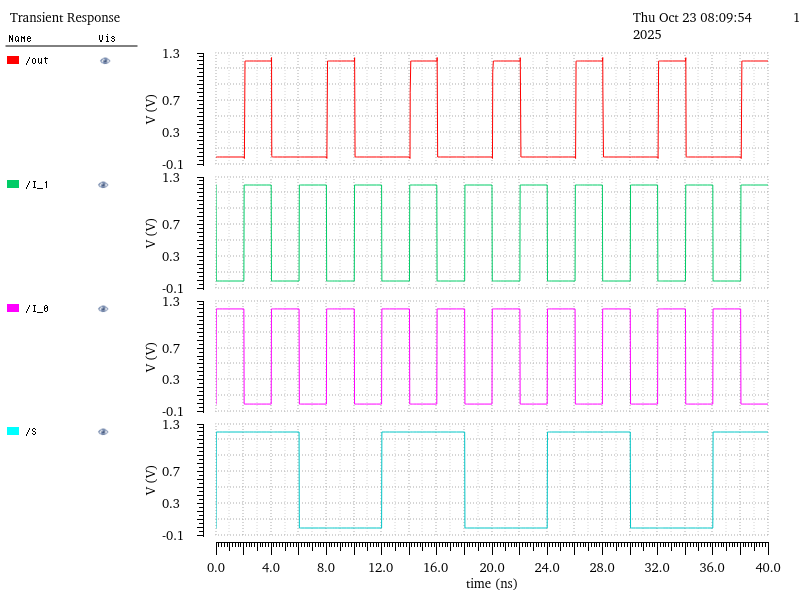
\includegraphics[width=0.5\linewidth]{writeup//figures/muxsubval.png}
    \caption{Enter Caption}
\end{figure}

In the subcircuit test, the select input \( S \) is toggled while \( I_0 \) and \( I_1 \) run as independent square waves. 
Whenever \( S \) is high, the output waveform overlays \( I_1 \) with only a small propagation delay; whenever \( S \) is low, the output overlays \( I_0 \). 
Each handoff can be observed at the transitions of \( S \): during every \( S=1 \) interval the output \( V_{\text{out}} \) matches \( I_1 \), and during every \( S=0 \) interval it matches \( I_0 \). 
This behavior corresponds to the expected logic equation 
\[
V_{\text{out}} = S \cdot I_1 + \overline{S} \cdot I_0
\]
for a 2:1 pass-gate multiplexer. 
The simulation therefore verifies that the subcircuit operates correctly.

\subsubsection*{16:1 LUT Validation}
\begin{figure}[H]
    \centering
    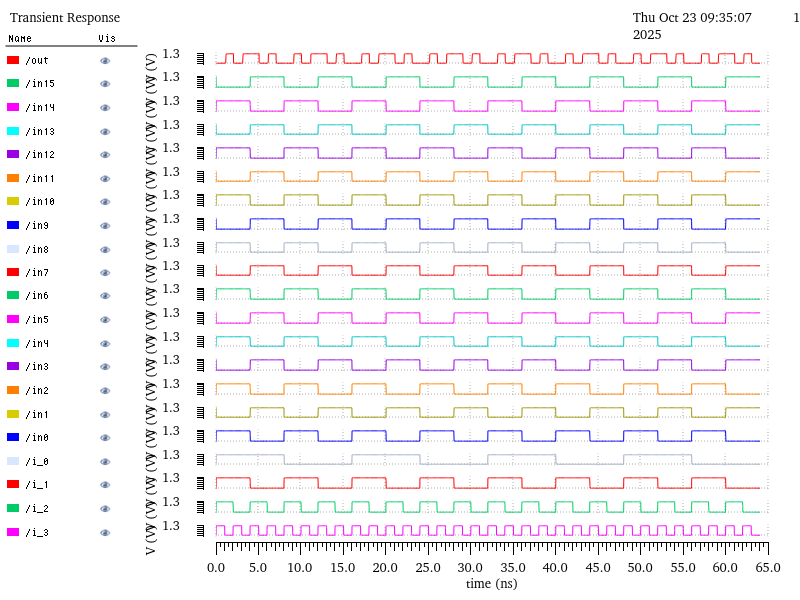
\includegraphics[width=0.5\linewidth]{writeup//figures/lutval.png}
    \caption{Enter Caption}
\end{figure}

For the full 16:1 LUT, all sixteen input combinations (\(2^4\)) were simulated by varying the four address lines from \(0000\) through \(1111\). 
In each address state, the output \(V_{\text{out}}\) aligns with exactly one corresponding data input. 
Specifically, when the address equals \(0000\), \(\text{IN}_0\) propagates to the output; as the address increments, \(\text{IN}_1, \text{IN}_2, \ldots, \text{IN}_{15}\) sequentially drive the output. 
Rising and falling edges on \(V_{\text{out}}\) coincide precisely with the selected input, while nonselected inputs show no coupling. 
Because all address combinations were verified and the output correctly reflected the selected data input each time, the 16:1 LUT simulation confirms correct functionality.

\newpage

% ------------------ SECTION 3 ------------------
\section{Baseline Delay Measurement}
\subsection{Test Schematic}

\begin{figure}[H]
    \centering
    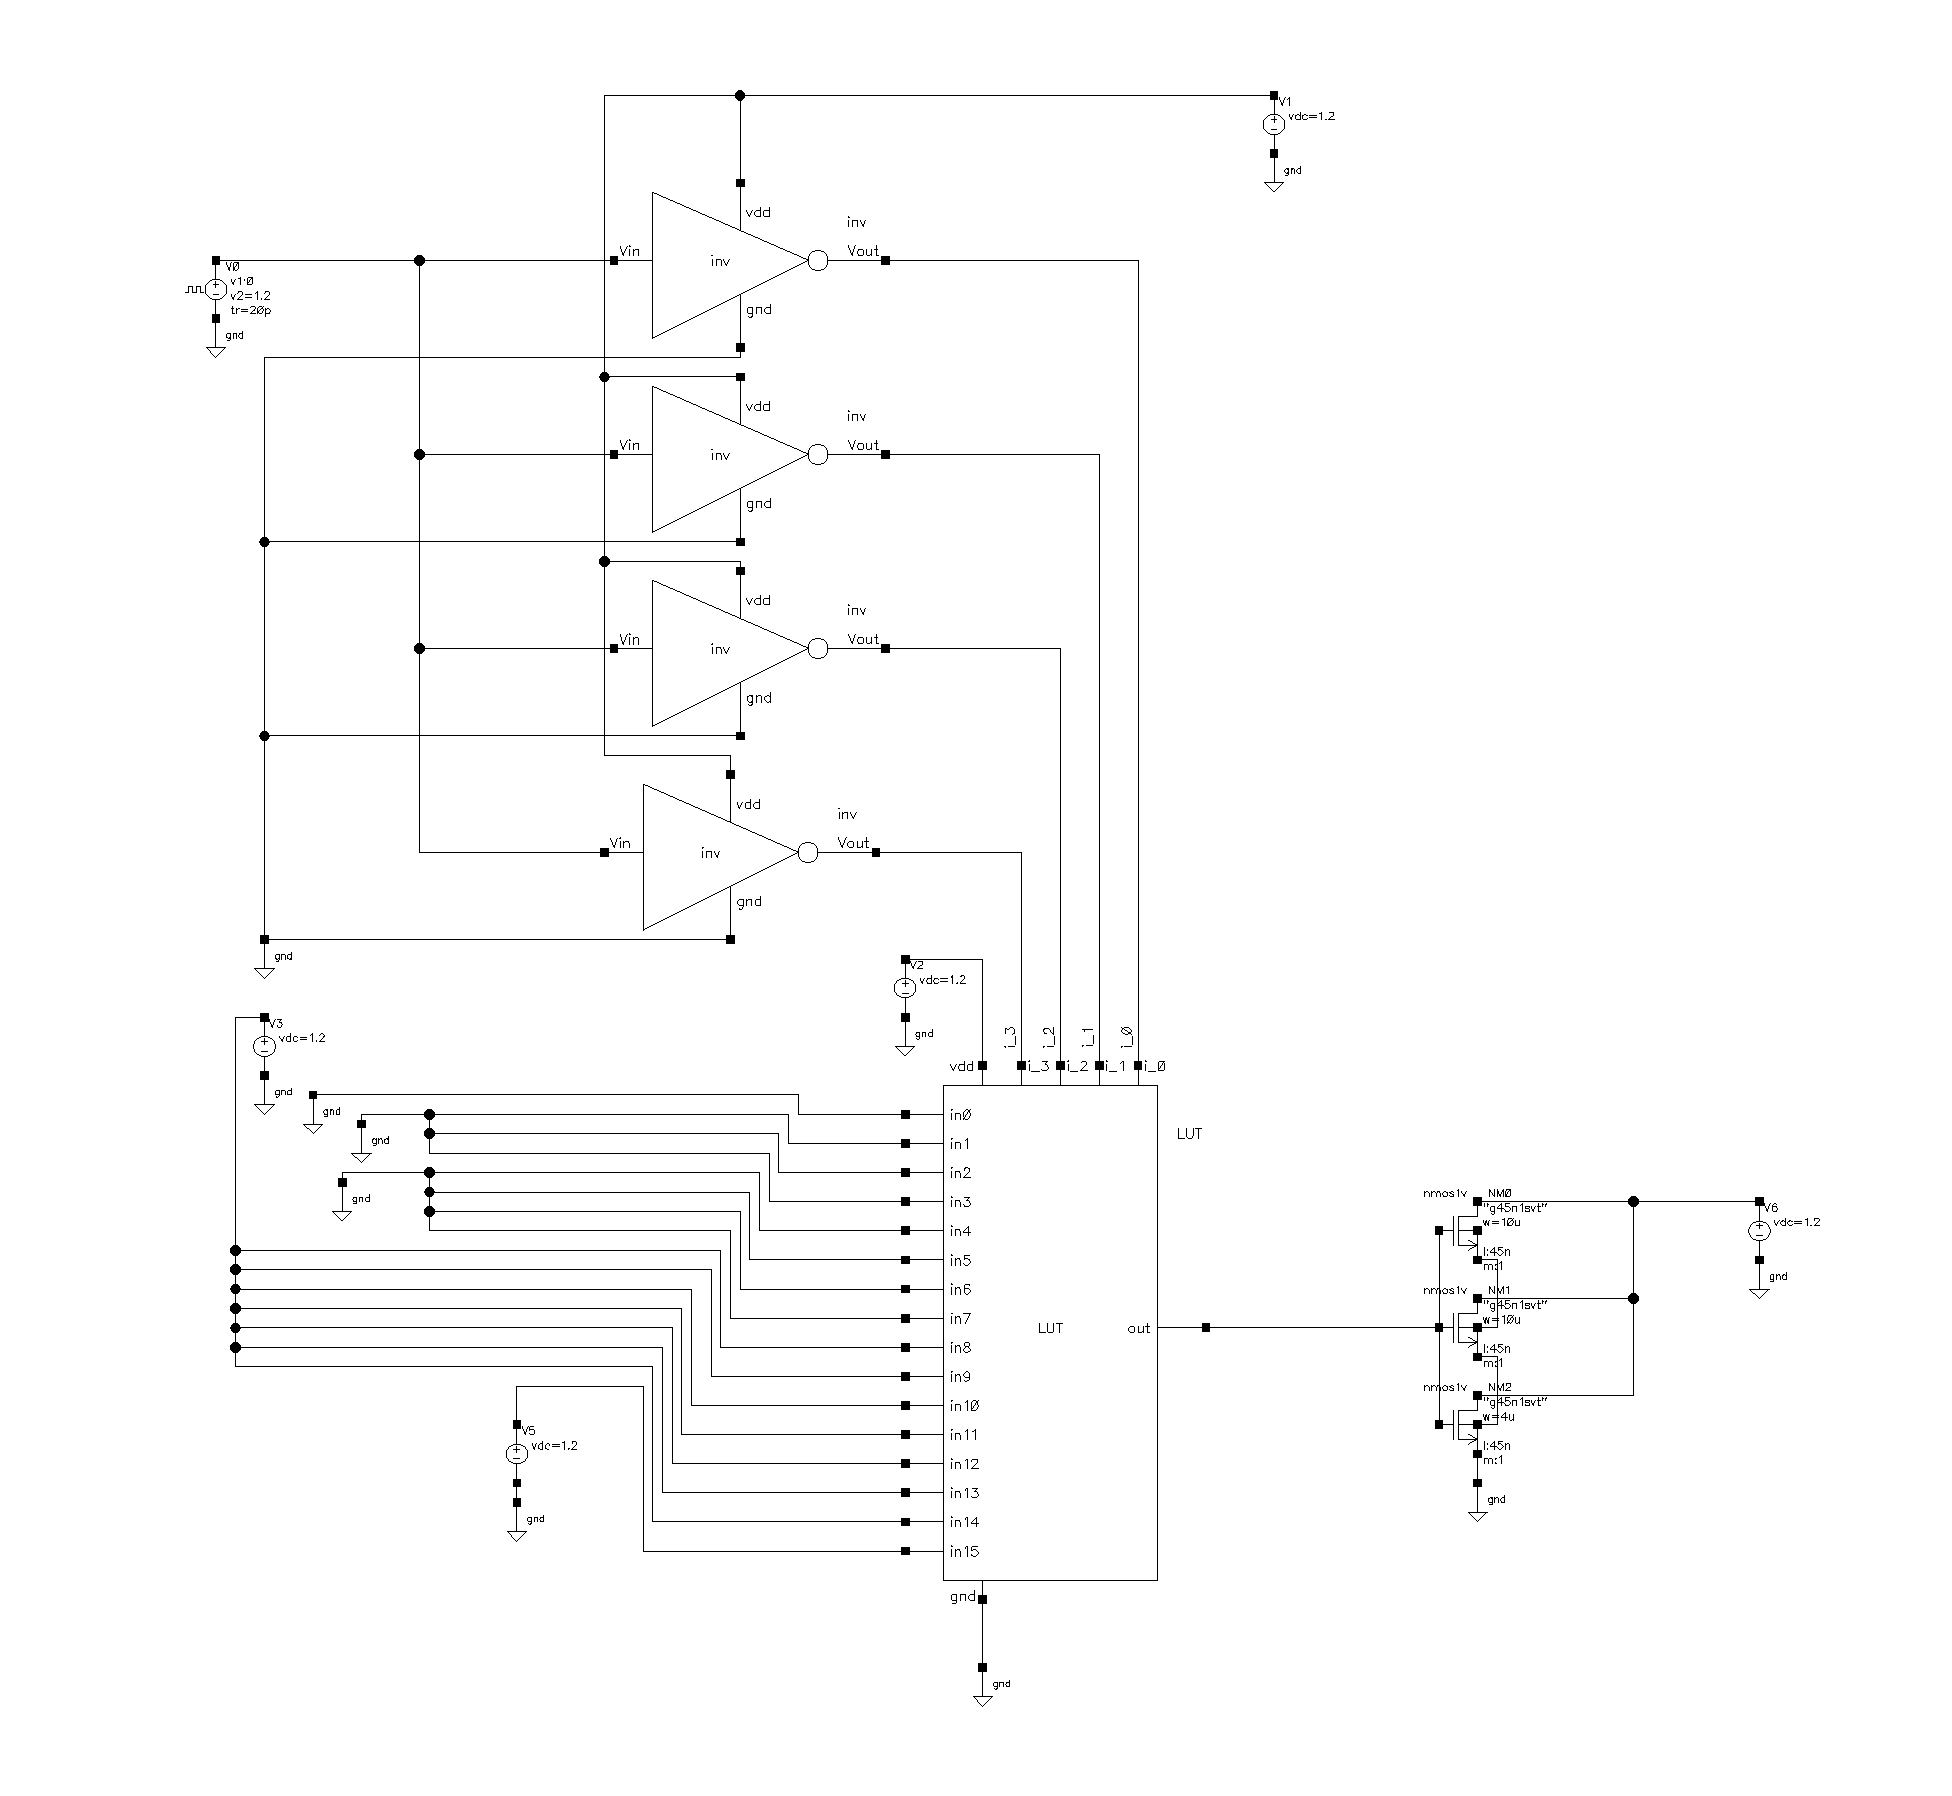
\includegraphics[width=0.5\linewidth]{writeup//figures/lut_delay_testbench.png}
    \caption{Enter Caption}
\end{figure}

\subsection{Test Case}
To evaluate the worst-case propagation delay of the 16:1 LUT, the input configuration was chosen to isolate the longest signal path through the multiplexer tree. 
Data inputs \(\text{IN}_0\) through \(\text{IN}_7\) were tied to ground (\(0\,\text{V}\)), while \(\text{IN}_8\) through \(\text{IN}_{15}\) were connected to \(V_{DD}\). 
Separate ground and \(V_{DD}\) connections were provided for \(\text{IN}_0\) and \(\text{IN}_{15}\), since these represent the boundary input cases that the output \(V_{\text{out}}\) would follow depending on the address configuration under test. 

The four address lines (\(I_0, I_1, I_2, I_3\)) were driven by \texttt{Vpulse} sources transitioning from low to high, generating the binary address sequence from \(0000\) to \(1111\). 
Switching all address inputs from 0 to 1 allowed the LUT to traverse every possible address combination, ensuring that the output response was tested across the full range of input states. 
This transition sequence also activates the critical switching path, as multiple internal MUX stages change simultaneously, causing maximum internal toggling and delay. 
Because \(I_3\) acted as the least significant bit (LSB), the signal path corresponding to \(I_3\) produced the longest propagation path through the multiplexer hierarchy and thus determined the worst-case delay.

At the output node, three NMOS transistors with widths of \(10\,\mu\text{m}\), \(10\,\mu\text{m}\), and \(4\,\mu\text{m}\) were connected in parallel to form an equivalent capacitive loading of approximately \(200C_g\). 
Given the minimum device width of \(120\,\text{nm}\), a total effective width of \(24\,\mu\text{m}\) was required to achieve this load. 
This output loading condition ensured realistic delay measurement under high fan-out, enabling accurate evaluation of the LUT’s timing performance in its worst-case switching scenario.

\newpage

\subsection{Simulation Results and Metric Value}
\begin{figure}[H]
    \centering
    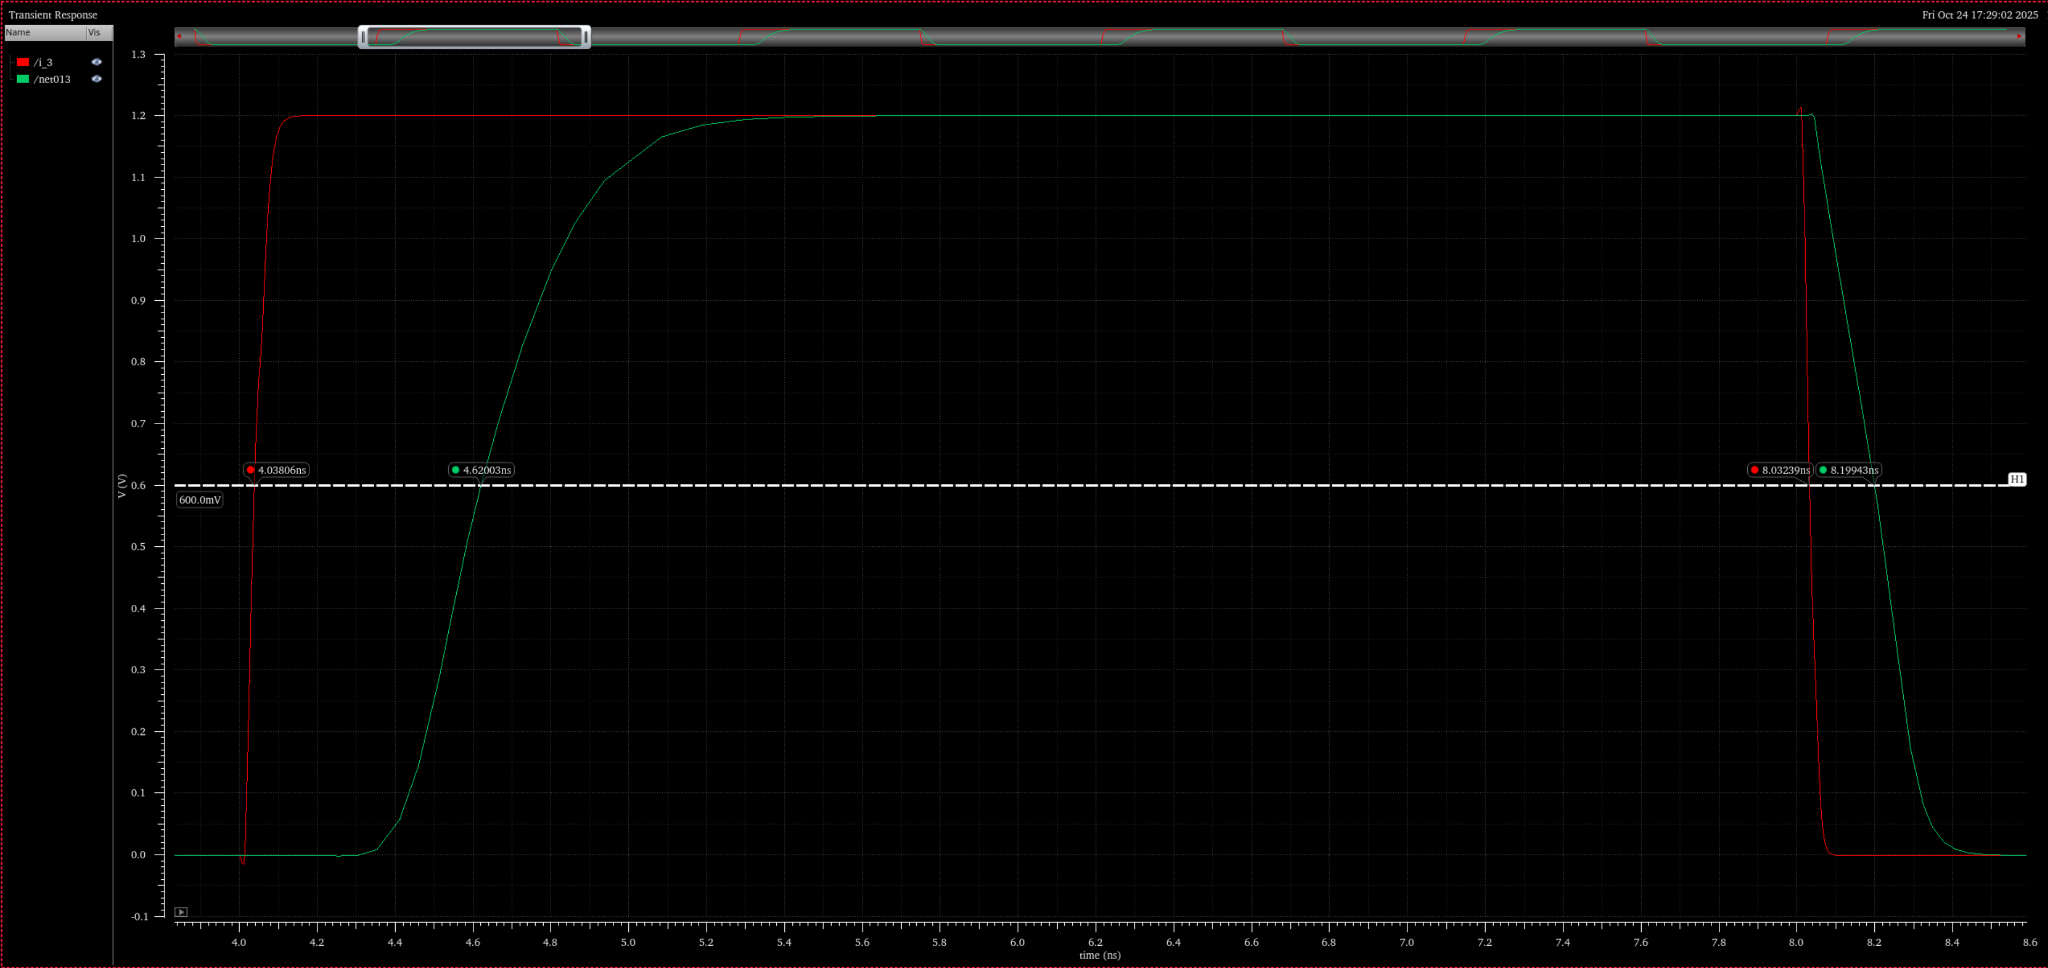
\includegraphics[width=0.5\linewidth]{writeup//figures/baselinedelay.png}
    \caption{Enter Caption}
\end{figure}
Propagation delay measurements are made at the 50\% voltage level of both the input and output signals, which corresponds to \( V = 0.5V_{DD} = 0.6\,\text{V} \) for a 1.2\,V supply.

\subsubsection*{Low-to-High Transition (\(t_{PLH}\))}

For the rising output transition:
\[
t_{PLH} = t_{\text{out,50\%↑}} - t_{\text{in,50\%↓}}
\]
Substituting measured values from the transient response:
\[
t_{PLH} = 4.62003\,\text{ns} - 4.03806\,\text{ns} = 0.58197\,\text{ns}
\]

\subsubsection*{High-to-Low Transition (\(t_{PHL}\))}

For the falling output transition:
\[
t_{PHL} = t_{\text{out,50\%↓}} - t_{\text{in,50\%↑}}
\]
\[
t_{PHL} = 8.19943\,\text{ns} - 8.03239\,\text{ns} = 0.16704\,\text{ns}
\]

\subsubsection*{Average and Worst-Case Delay}

The average propagation delay is given by:
\[
t_p = \frac{t_{PLH} + t_{PHL}}{2}
\]
\[
t_p = \frac{0.58197 + 0.16704}{2} = 0.3745\,\text{ns}
\]

The worst-case delay is the longer of the two:
\[
t_{pd,worst} = \max(t_{PLH}, t_{PHL}) = 0.58197\,\text{ns}
\]

From the results, the rising transition (\(t_{PLH}\)) dominates, indicating that the PMOS network contributes more delay due to its higher effective resistance compared to the NMOS pull-down path. 
Therefore, the \textbf{worst-case propagation delay} of the circuit is approximately \(\mathbf{0.582\,ns}\).


\newpage

% ------------------ SECTION 4 ------------------
\section{Baseline Frequency Measurement}
\subsection{Test Schematic}

\begin{figure}[H]
    \centering
    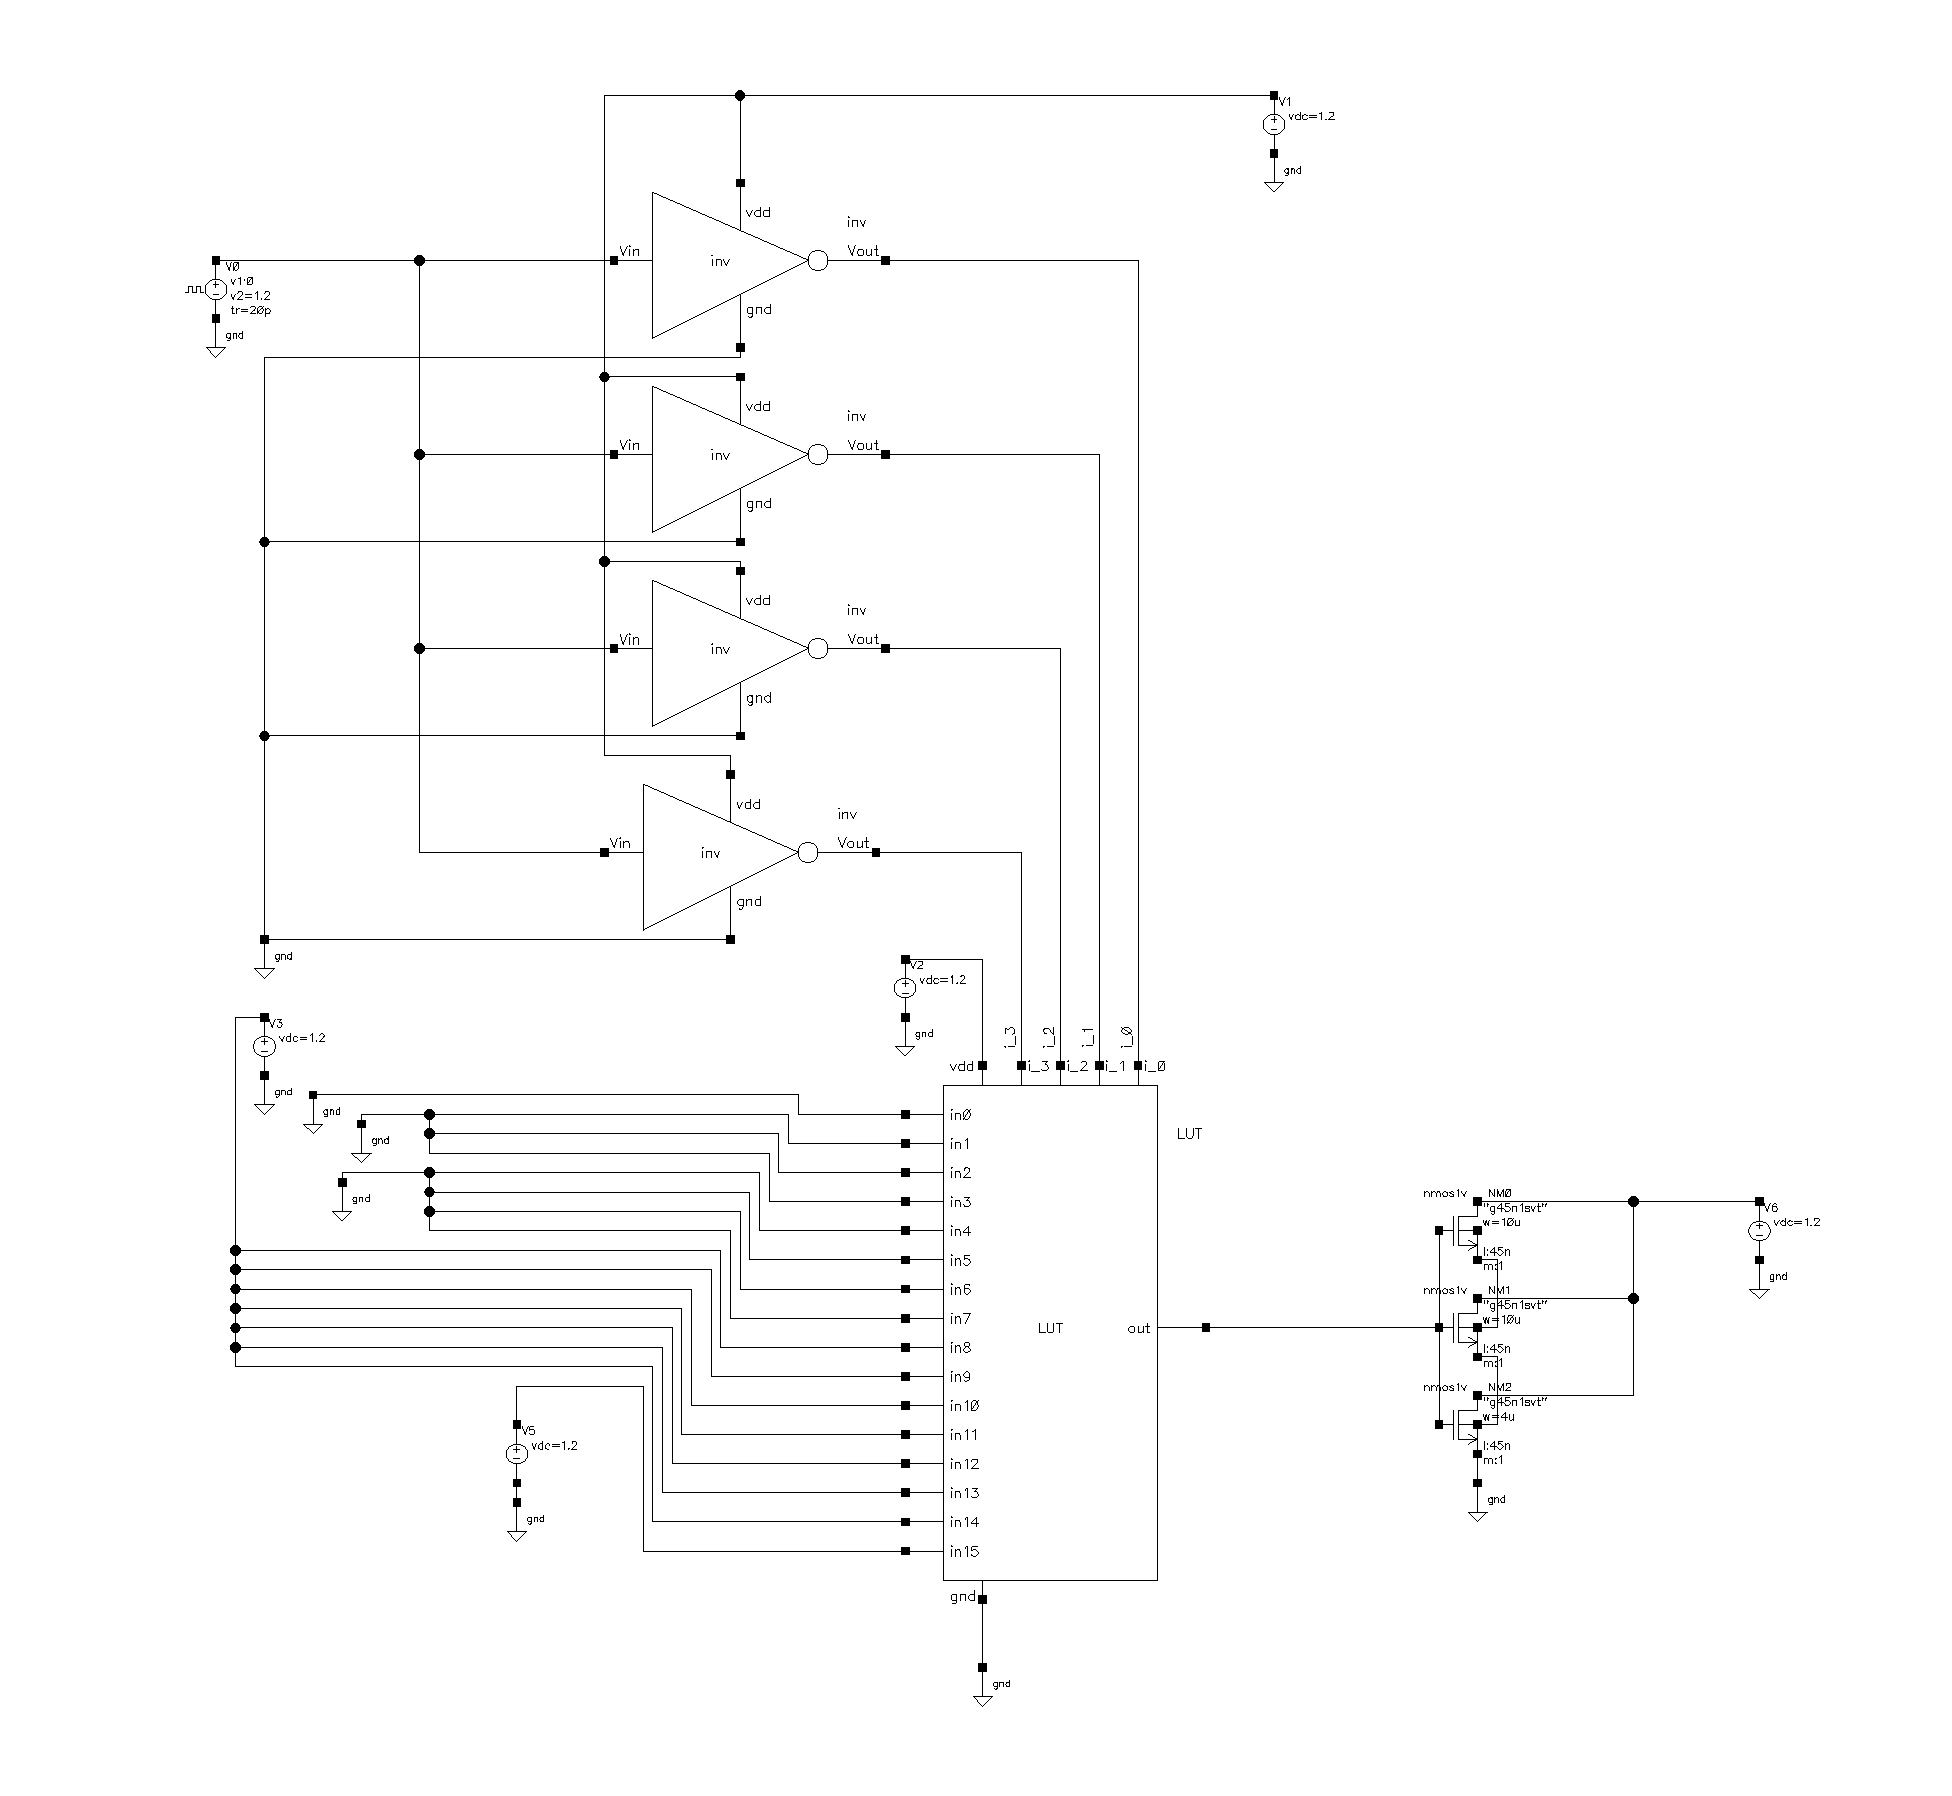
\includegraphics[width=0.5\linewidth]{writeup//figures/lut_delay_testbench.png}
    \caption{Enter Caption}
\end{figure}
We set the period of the Vpulse to be 1/f, where f is a variable that represents frequency. 


\newpage

\subsection{Simulation Results and Metric Value}

\begin{figure}[H]
    \centering
    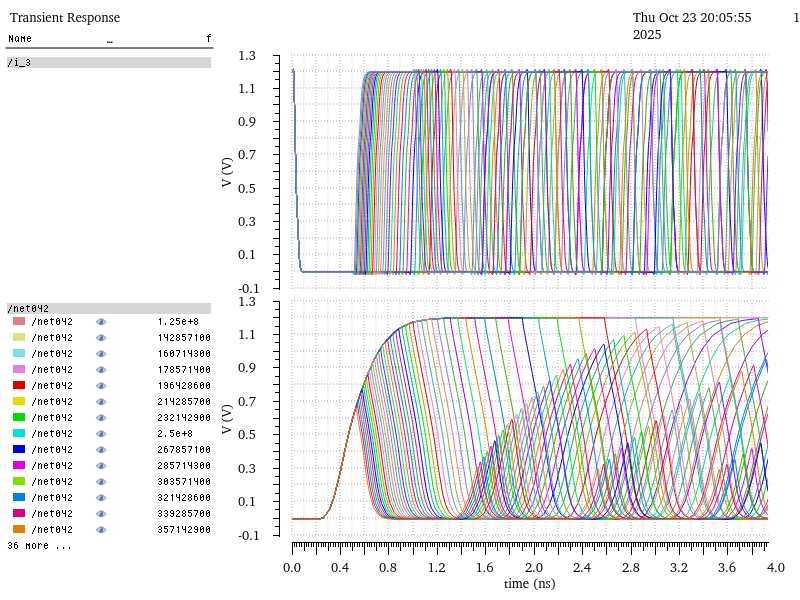
\includegraphics[width=0.75\linewidth]{writeup//figures/frequency_response_param.png}
    \caption{Frequency response at output of the buffer stage}
\end{figure}

\begin{figure}[H]
    \centering
    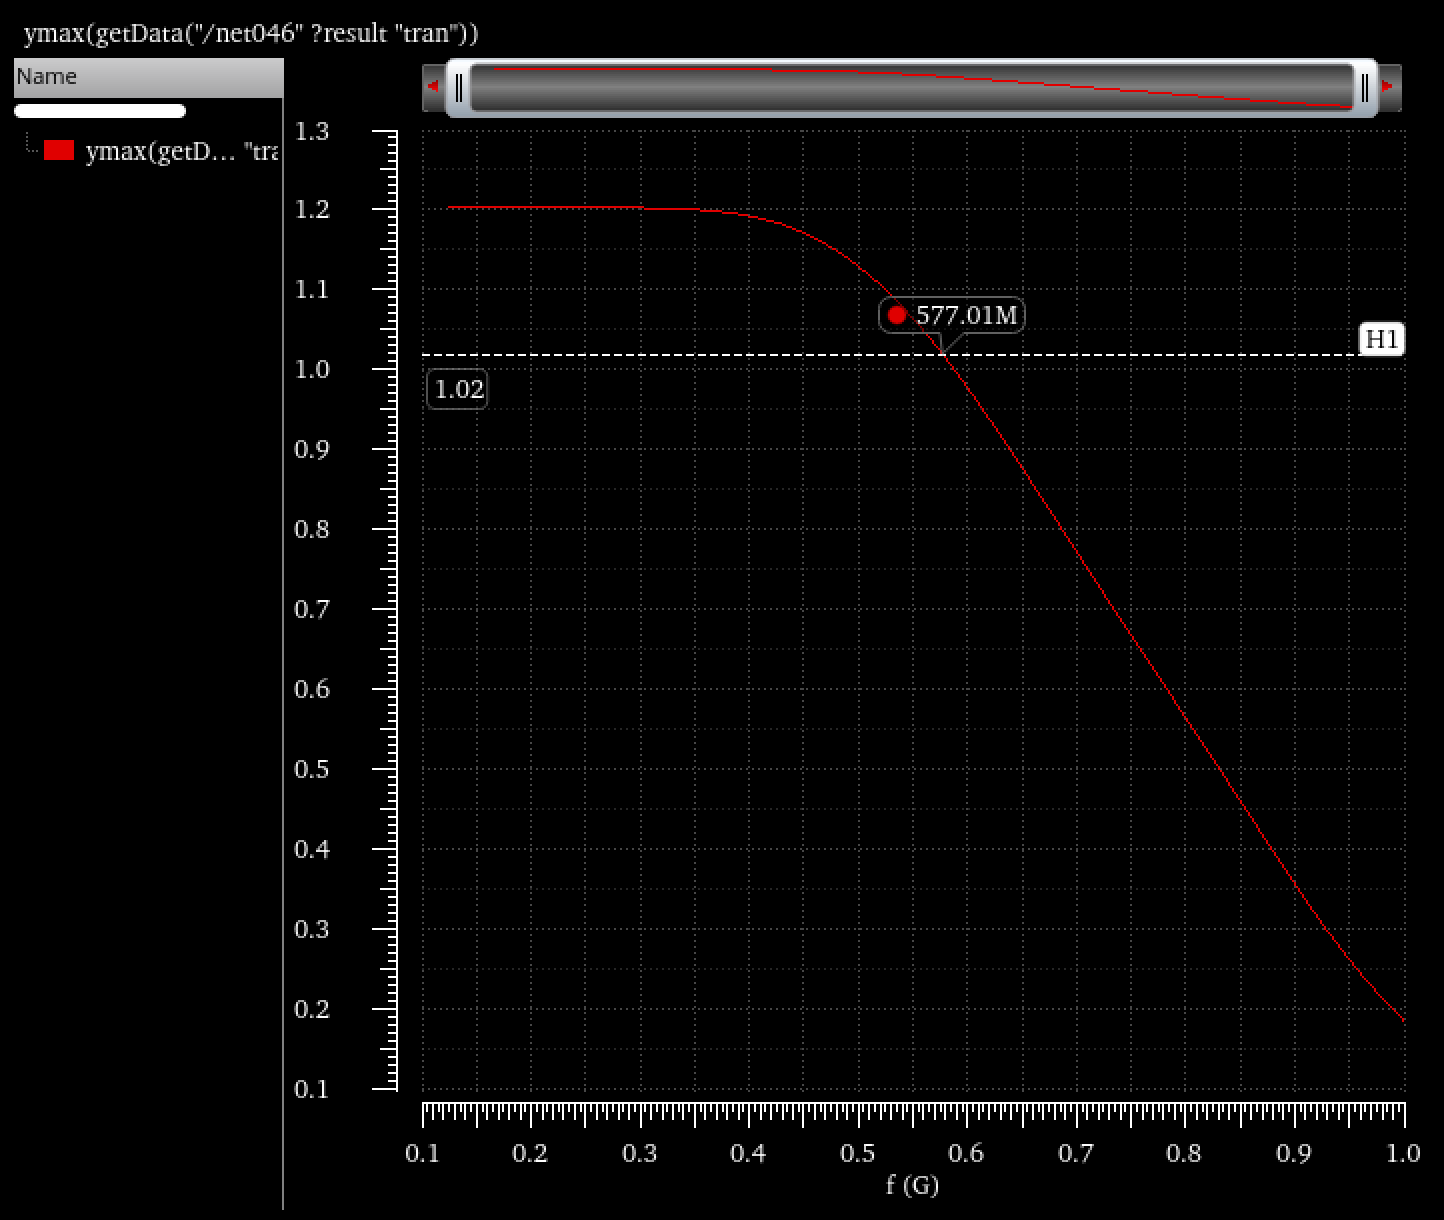
\includegraphics[width=0.75\linewidth]{writeup//figures/max_frequencies.png}
    \caption{Extracting frequency value that allows for 85\% of VDD after buffer stage}
\end{figure}

\newpage

% ------------------ SECTION 5 ------------------
\section{Baseline Energy Measurement}
\subsection{Test Schematic}

\begin{figure}[H]
    \centering
    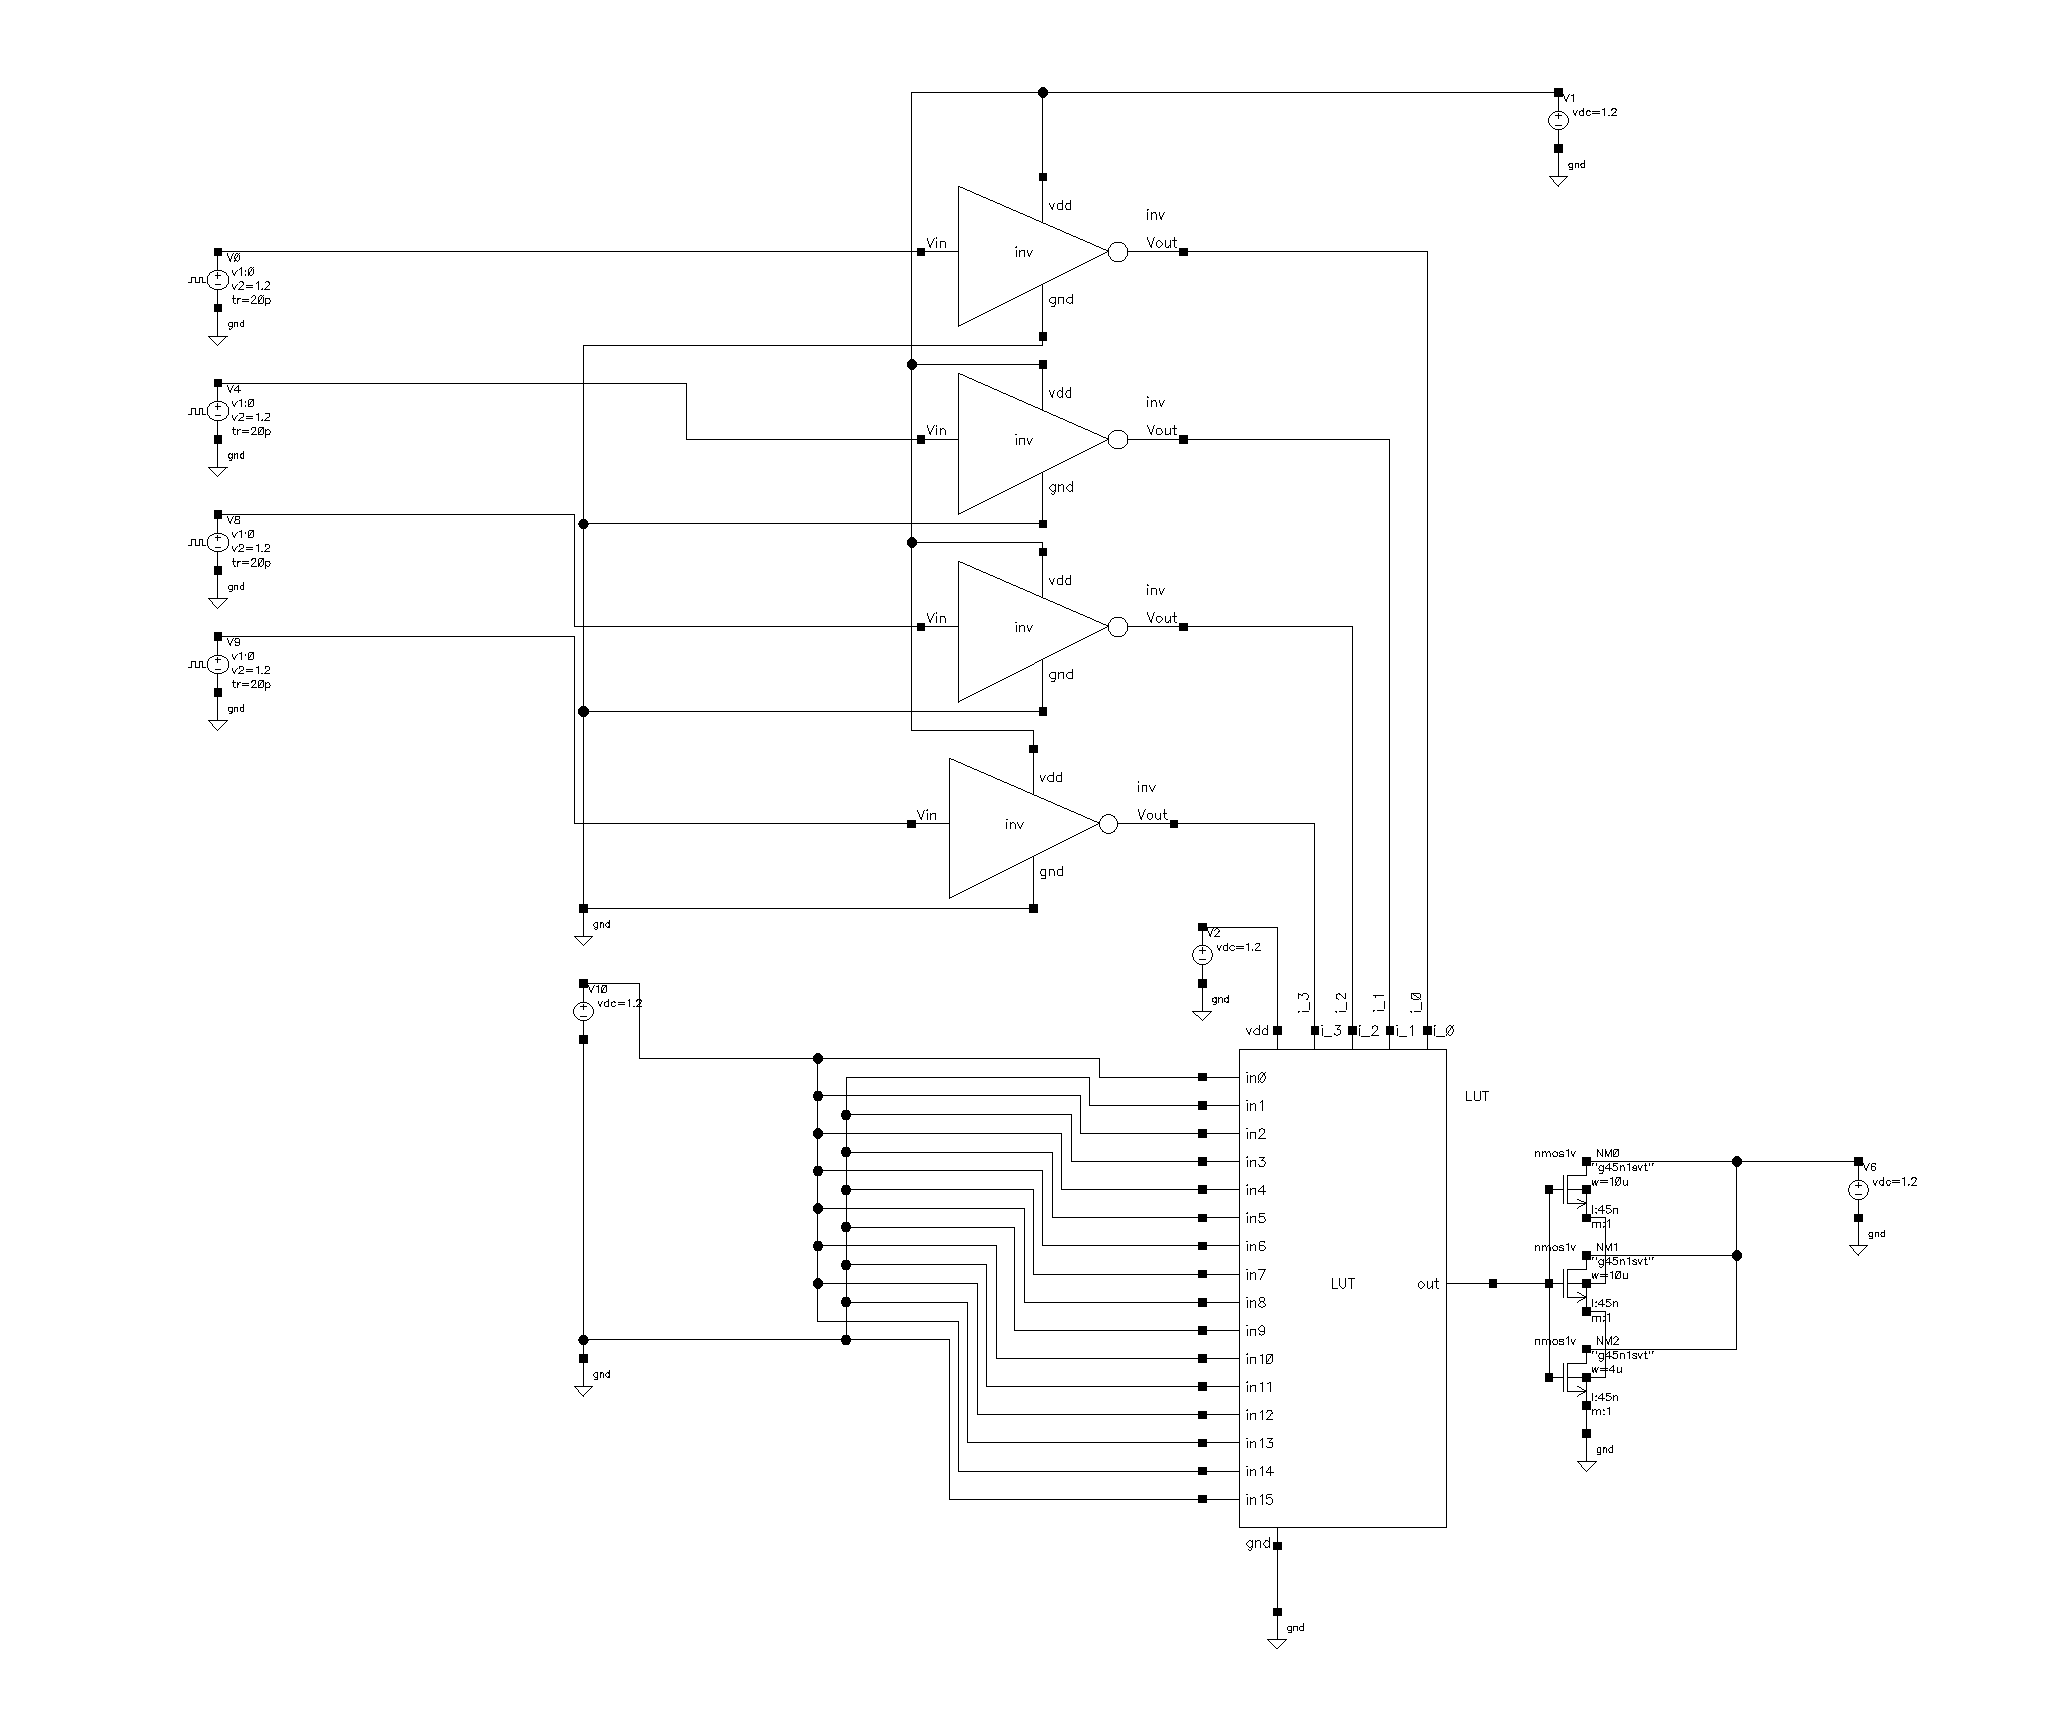
\includegraphics[width=0.75\linewidth]{writeup//figures/lut_energy_testbench.png}
    \caption{}
\end{figure}


\newpage

\subsection{Test Case}



\newpage

\subsection{Simulation Results and Metric Value}
\begin{figure}[H]
    \centering
    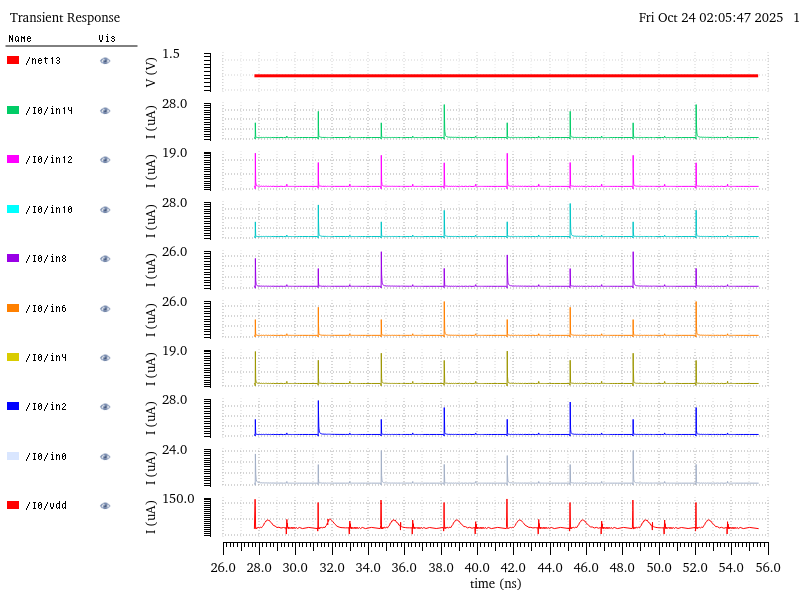
\includegraphics[width=0.5\linewidth]{writeup//figures/baseline_energy_currents.png}
    \caption{Enter Caption}
\end{figure}

\begin{figure}[H]
    \centering
    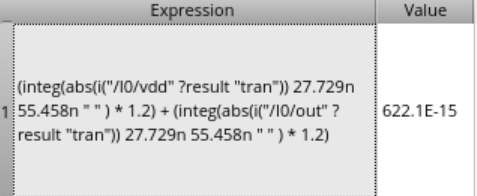
\includegraphics[width=0.5\linewidth]{writeup//figures/baseline_energy_val.png}
    \caption{Enter Caption}
\end{figure}

\newpage

% ------------------ SECTION 6 ------------------
\section{Optimized Design}
\subsection{Optimized Design Schematics}
\begin{figure}[H]
    \centering
    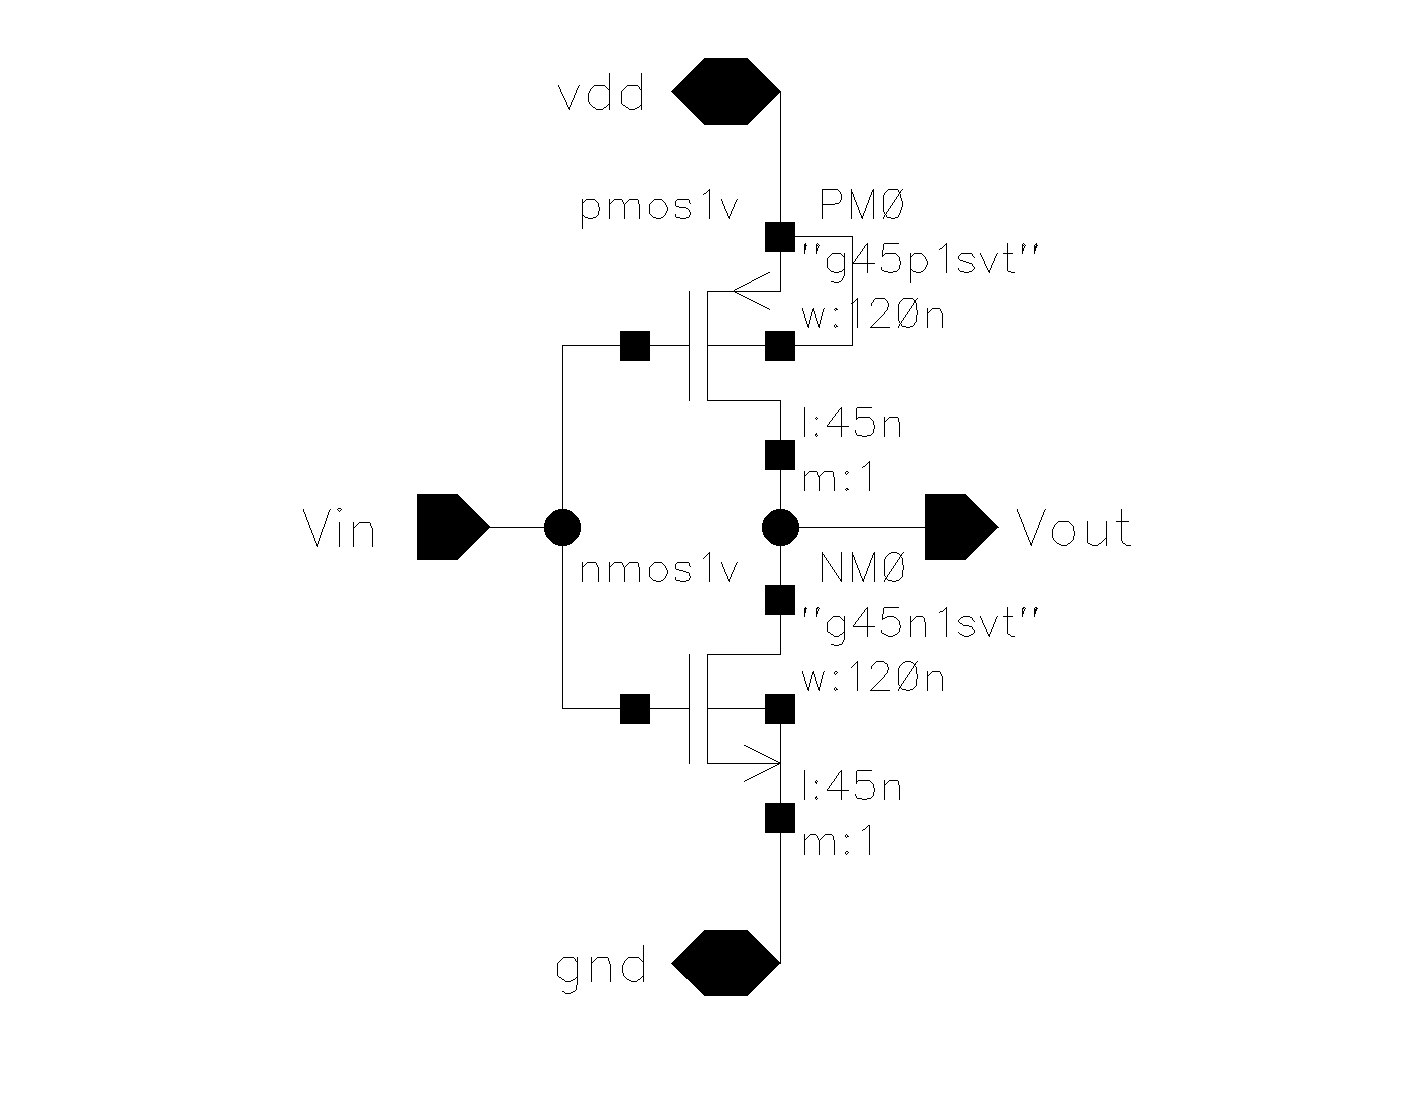
\includegraphics[width=0.5\linewidth]{writeup//figures/inv_sch.png}
    \caption{Enter Caption}
\end{figure}

\subsubsection*{Symbol}

\begin{figure}[H]
    \centering
    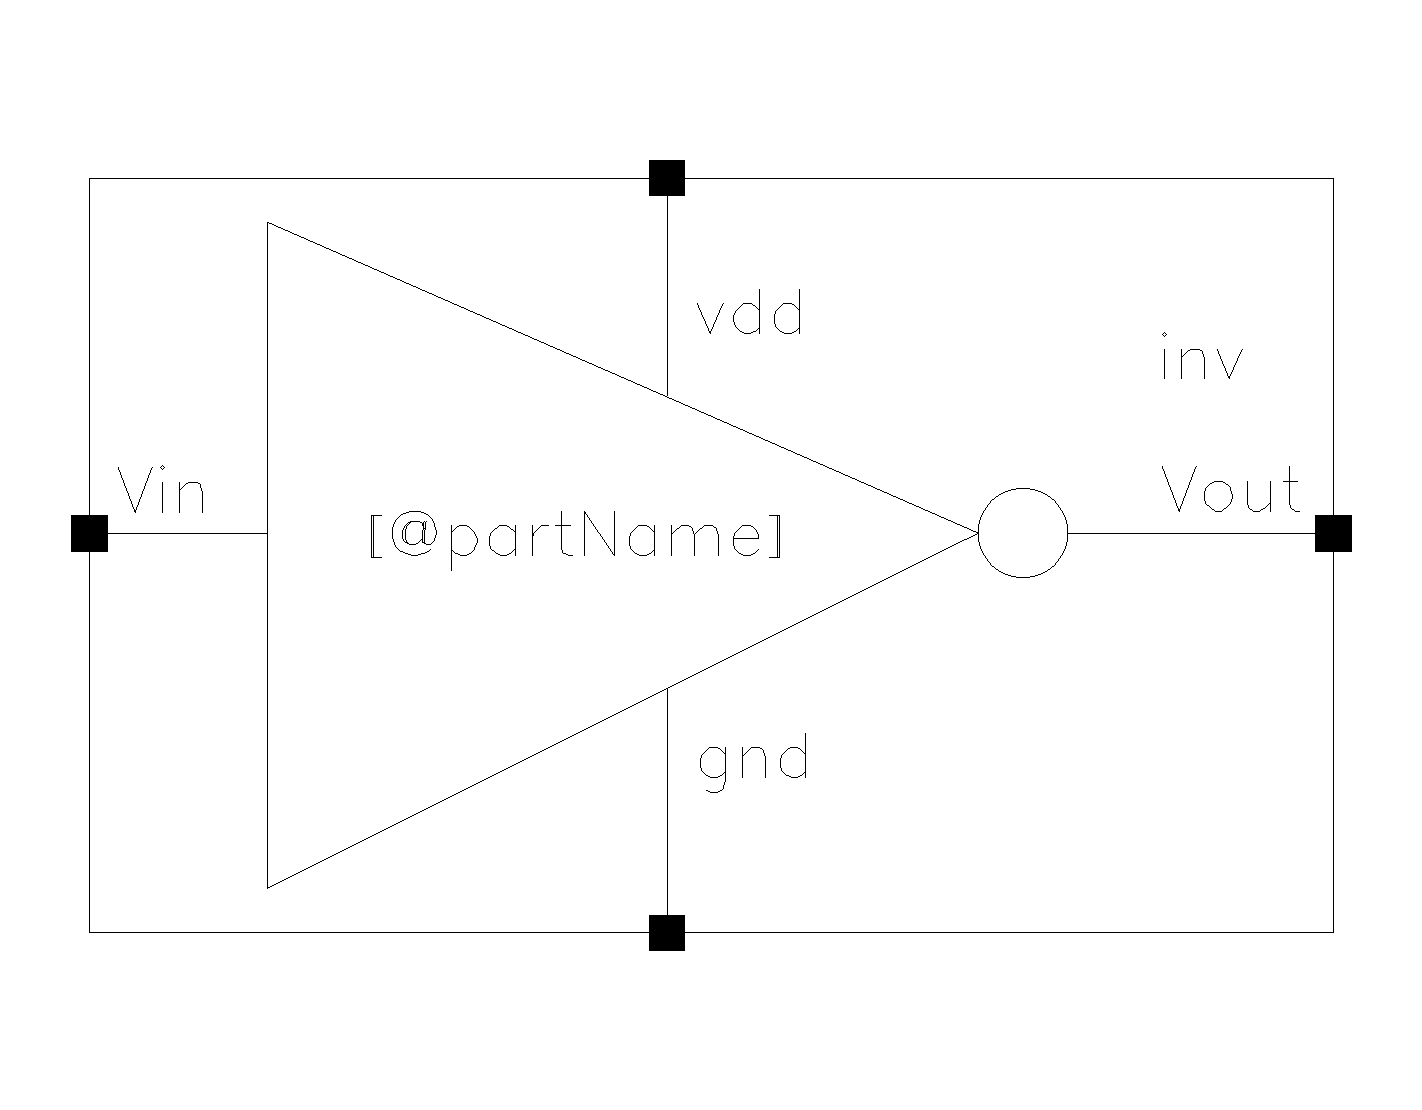
\includegraphics[width=0.5\linewidth]{writeup//figures/inv_sym.png}
    \caption{Enter Caption}
\end{figure}

\begin{figure}[H]
    \centering
    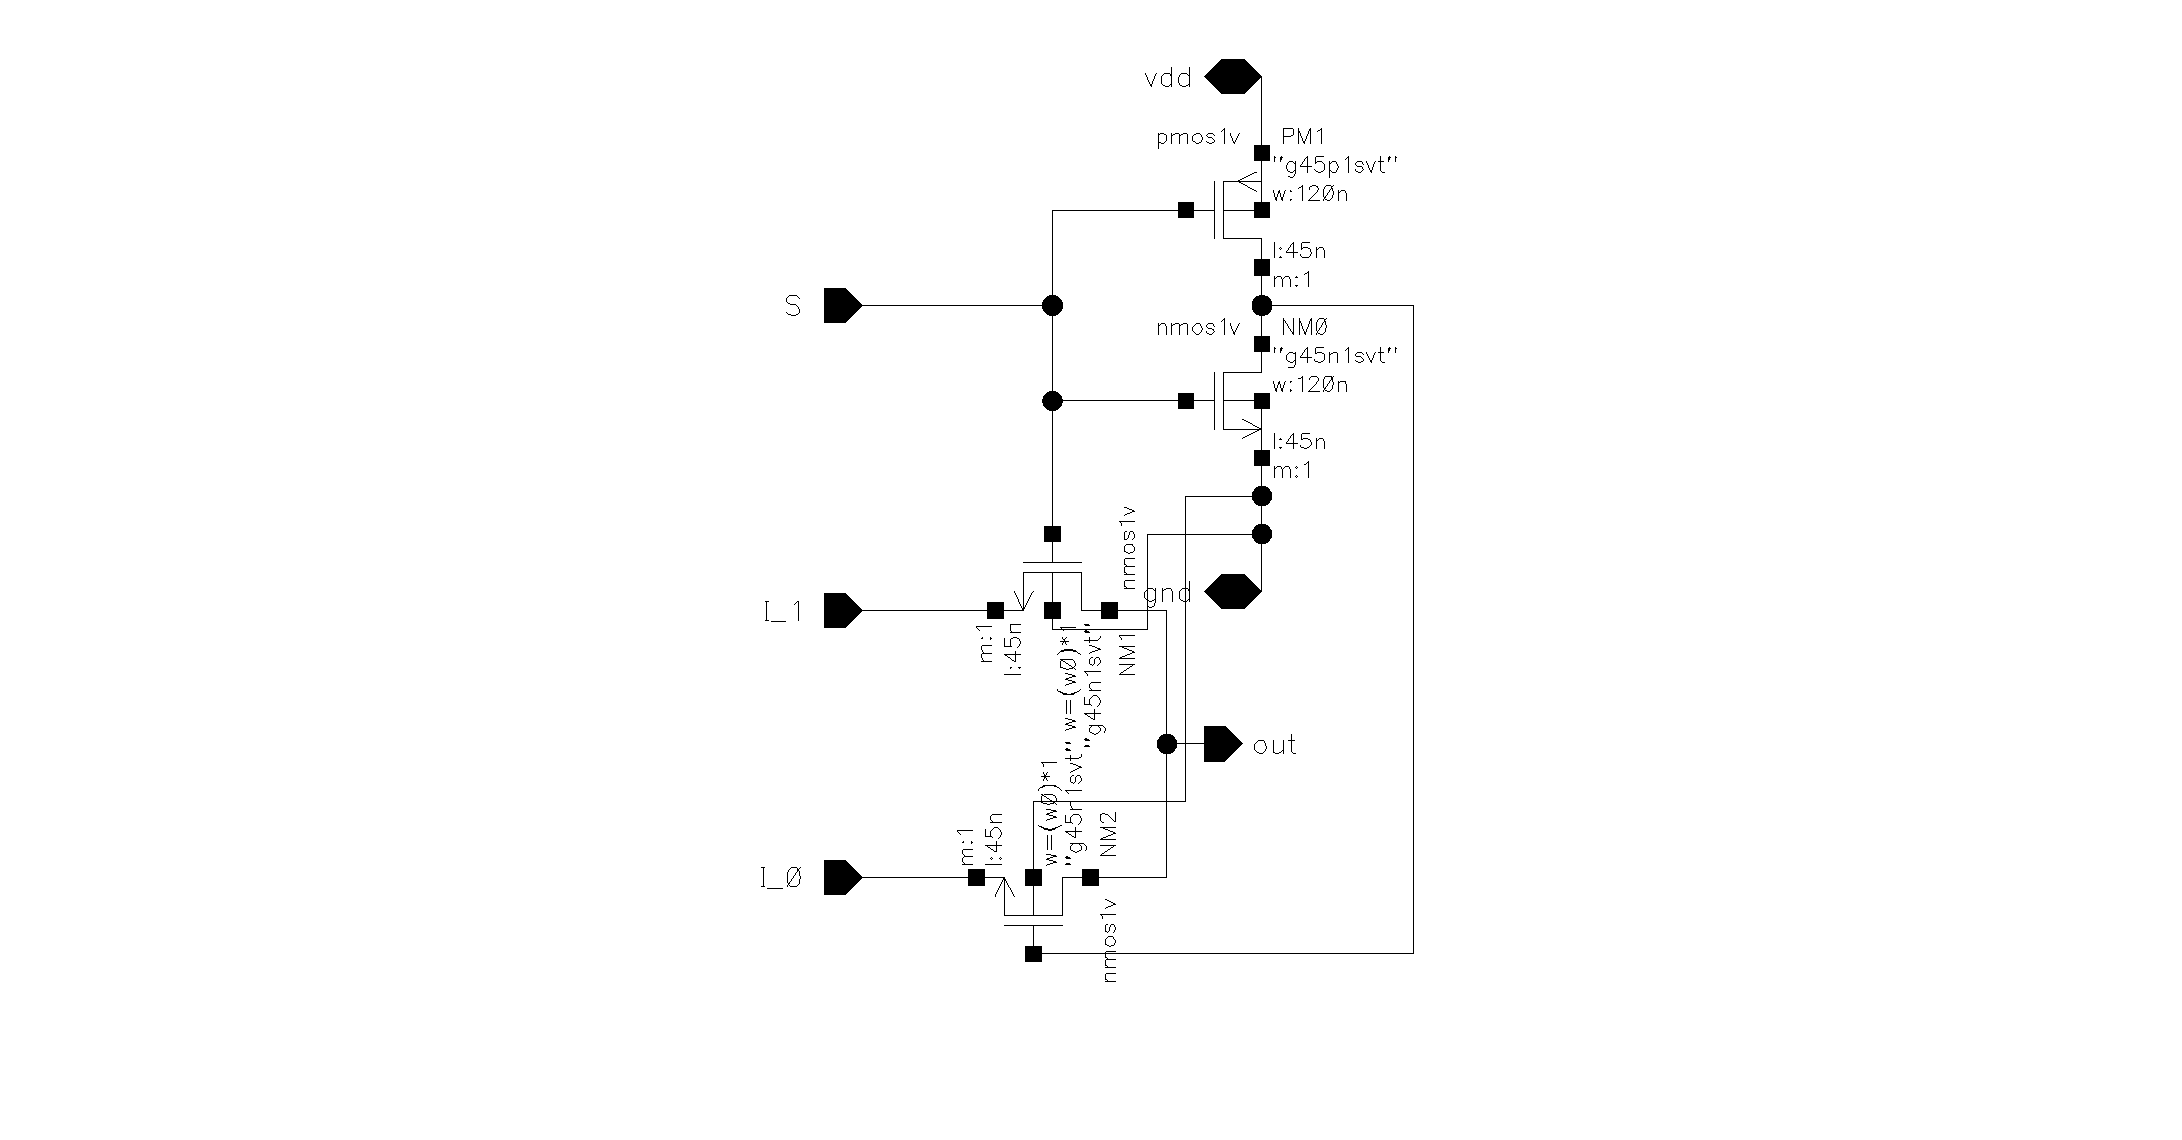
\includegraphics[width=0.5\linewidth]{writeup//figures/mux_w0_opt.png}
    \caption{Enter Caption}
\end{figure}

\begin{figure}[H]
    \centering
    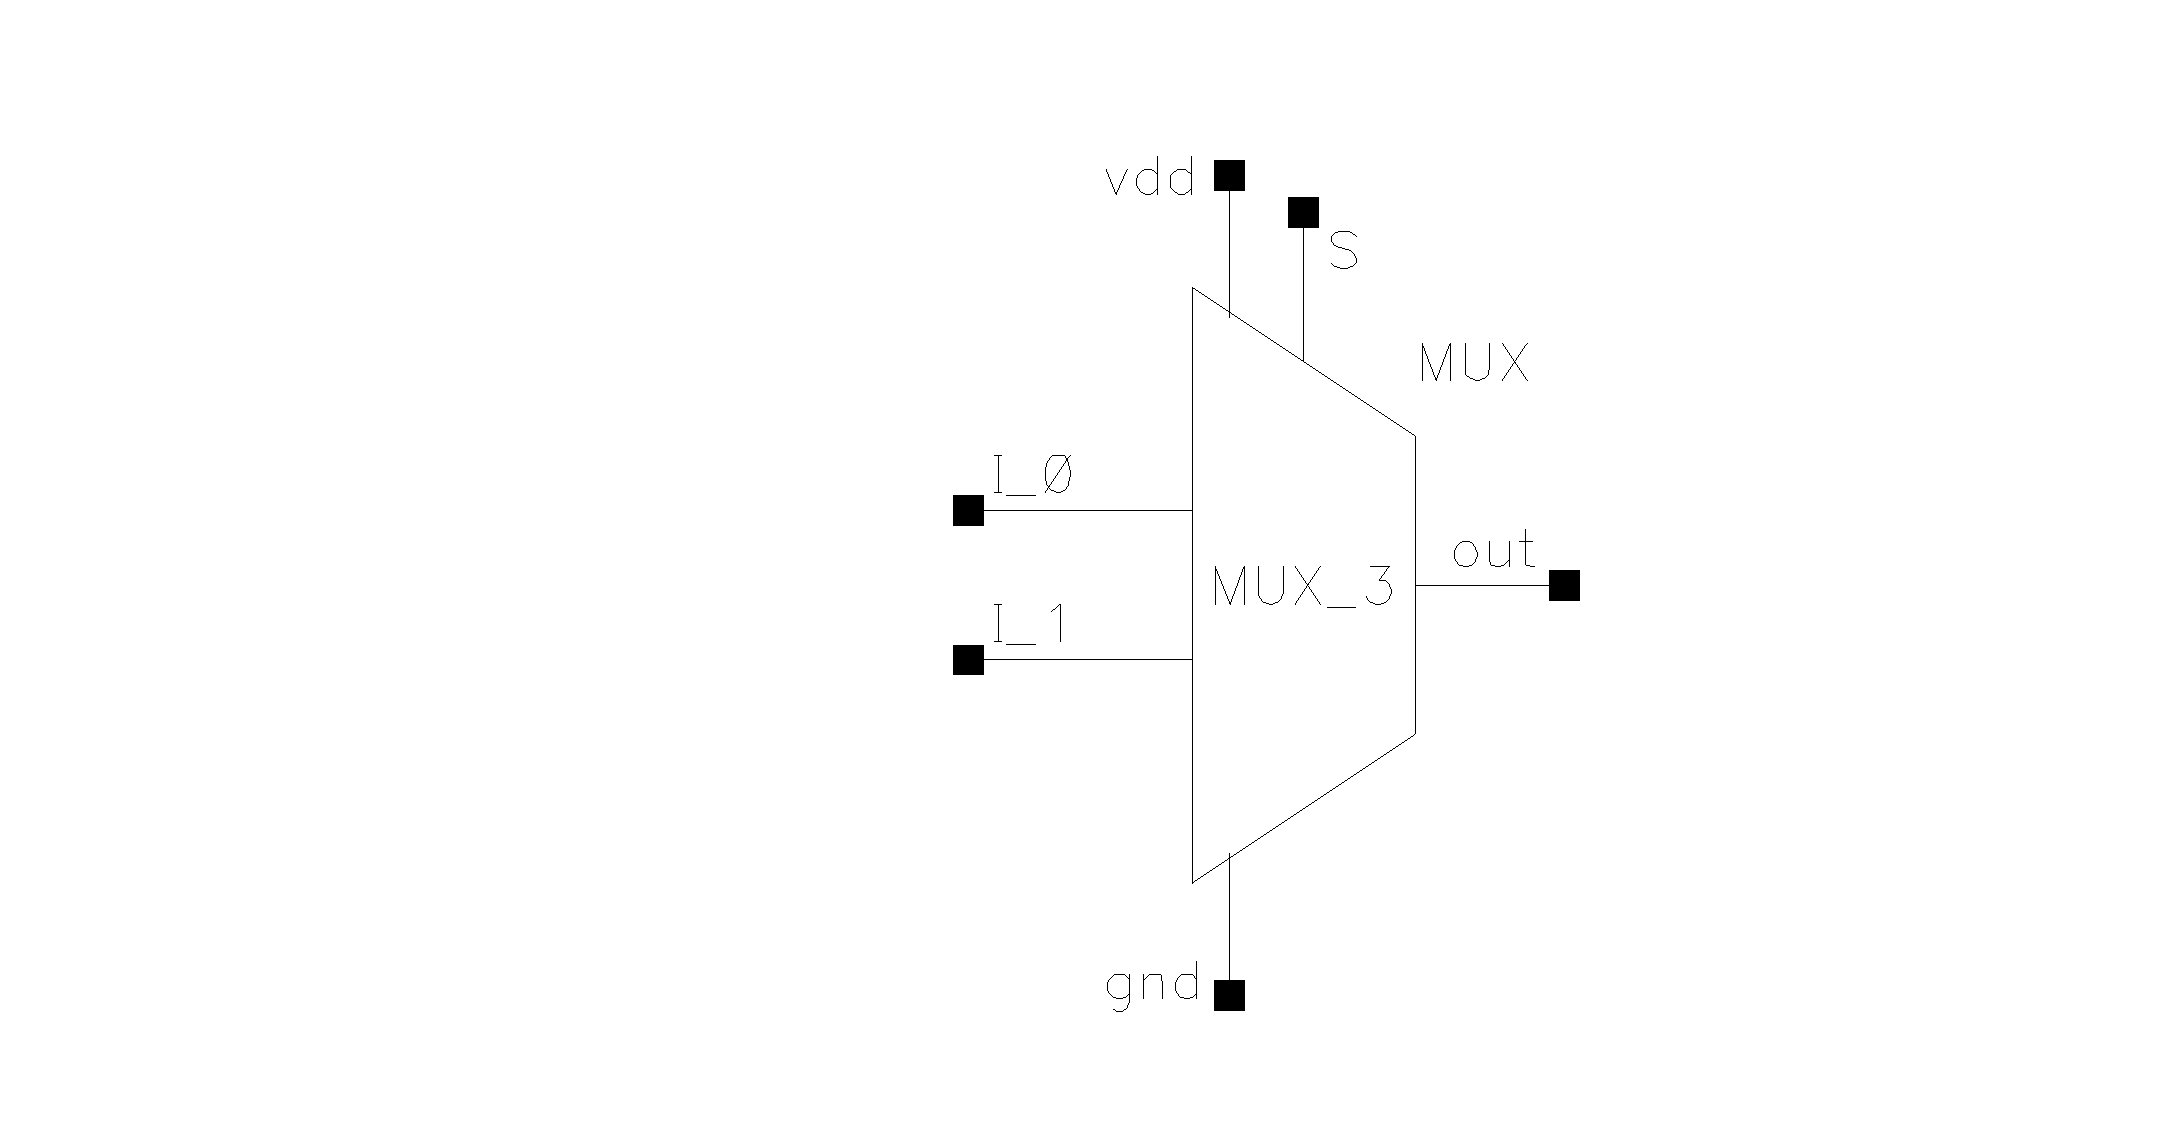
\includegraphics[width=0.5\linewidth]{writeup//figures/mux_w0_opt_sym.png}
    \caption{Enter Caption}
\end{figure}

\begin{figure}[H]
    \centering
    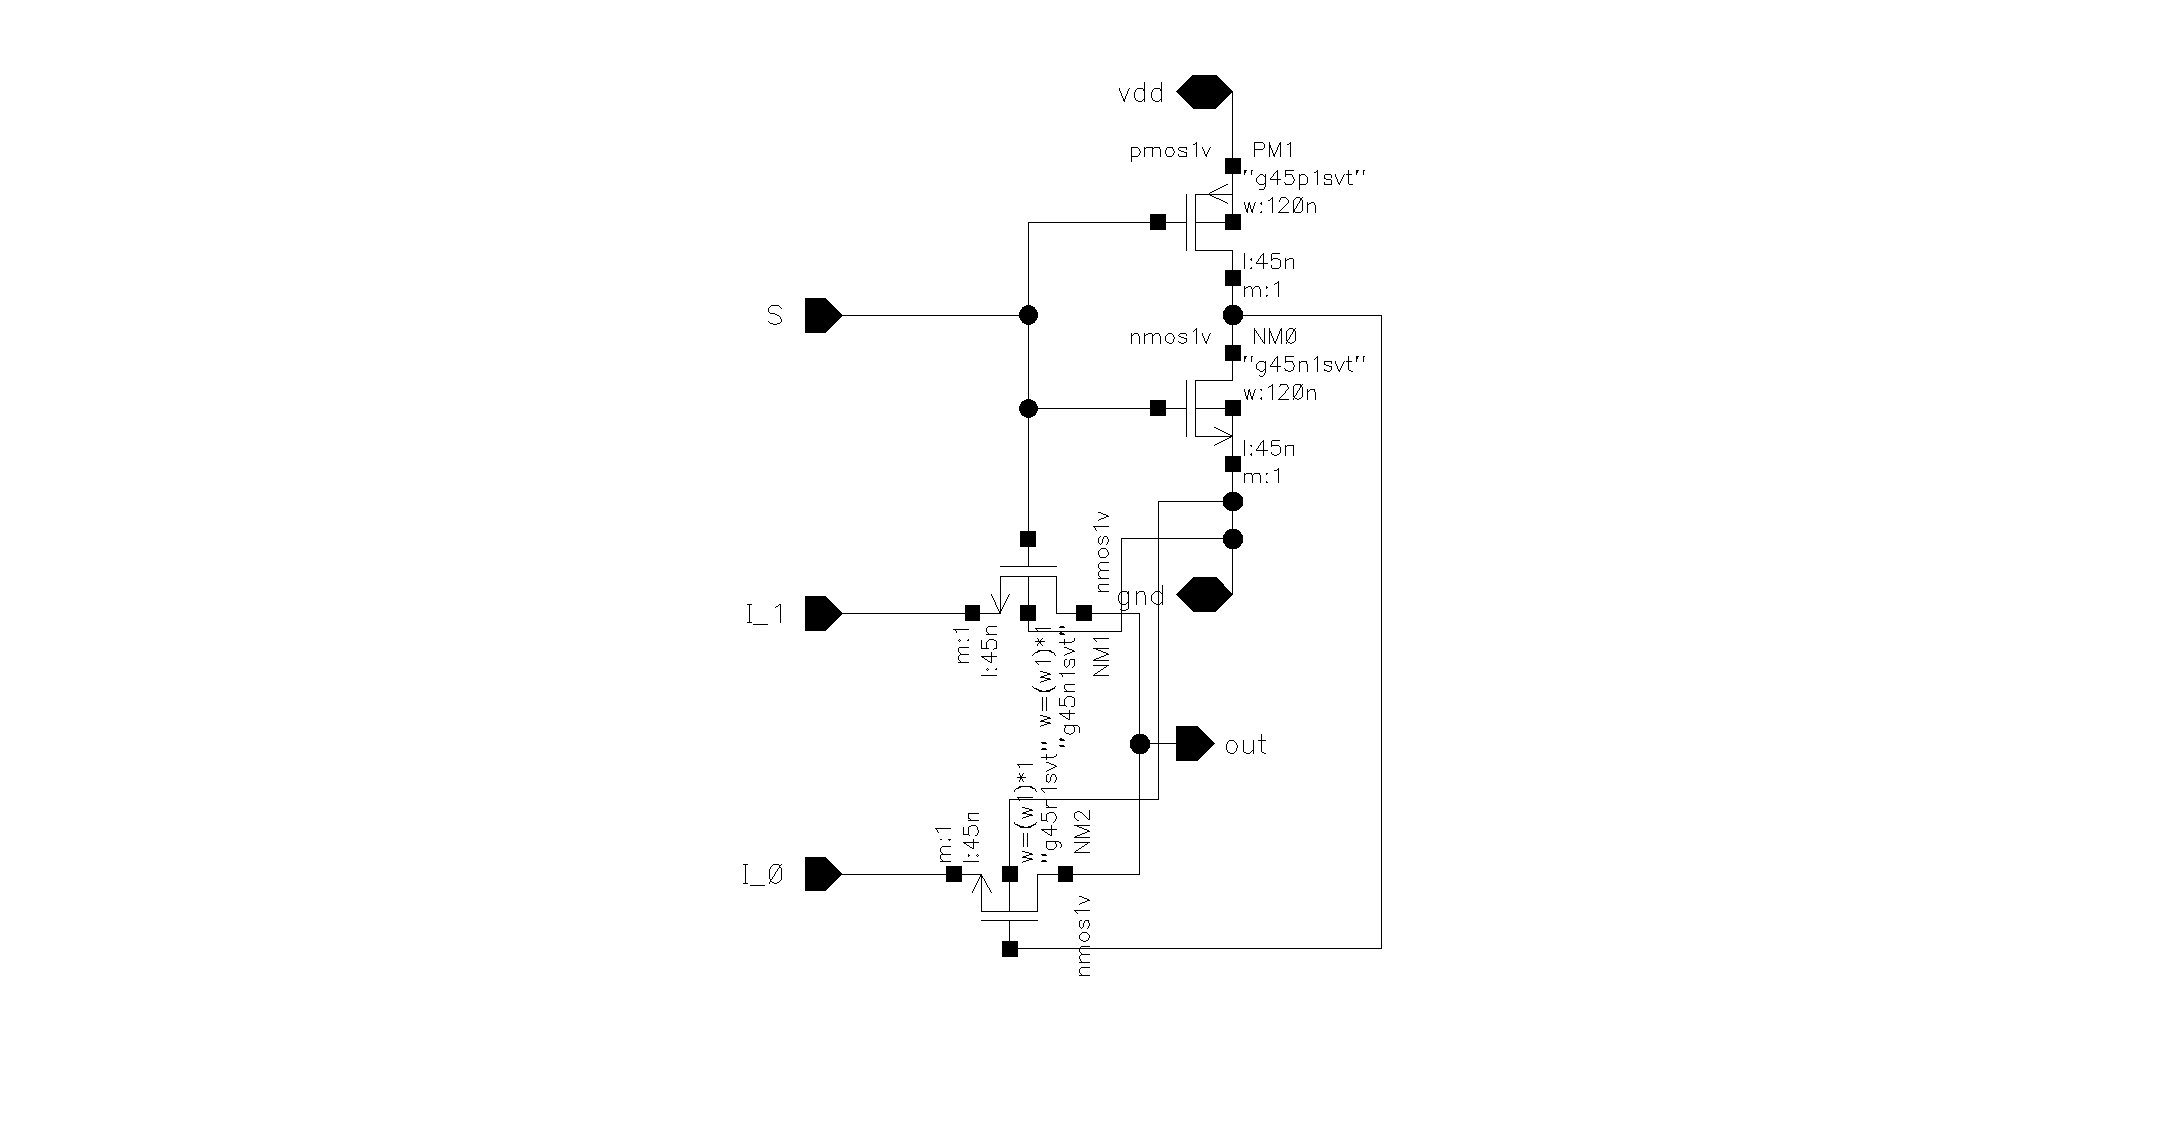
\includegraphics[width=0.5\linewidth]{writeup//figures/mux_w1_opt.png}
    \caption{Enter Caption}
\end{figure}

\begin{figure}[H]
    \centering
    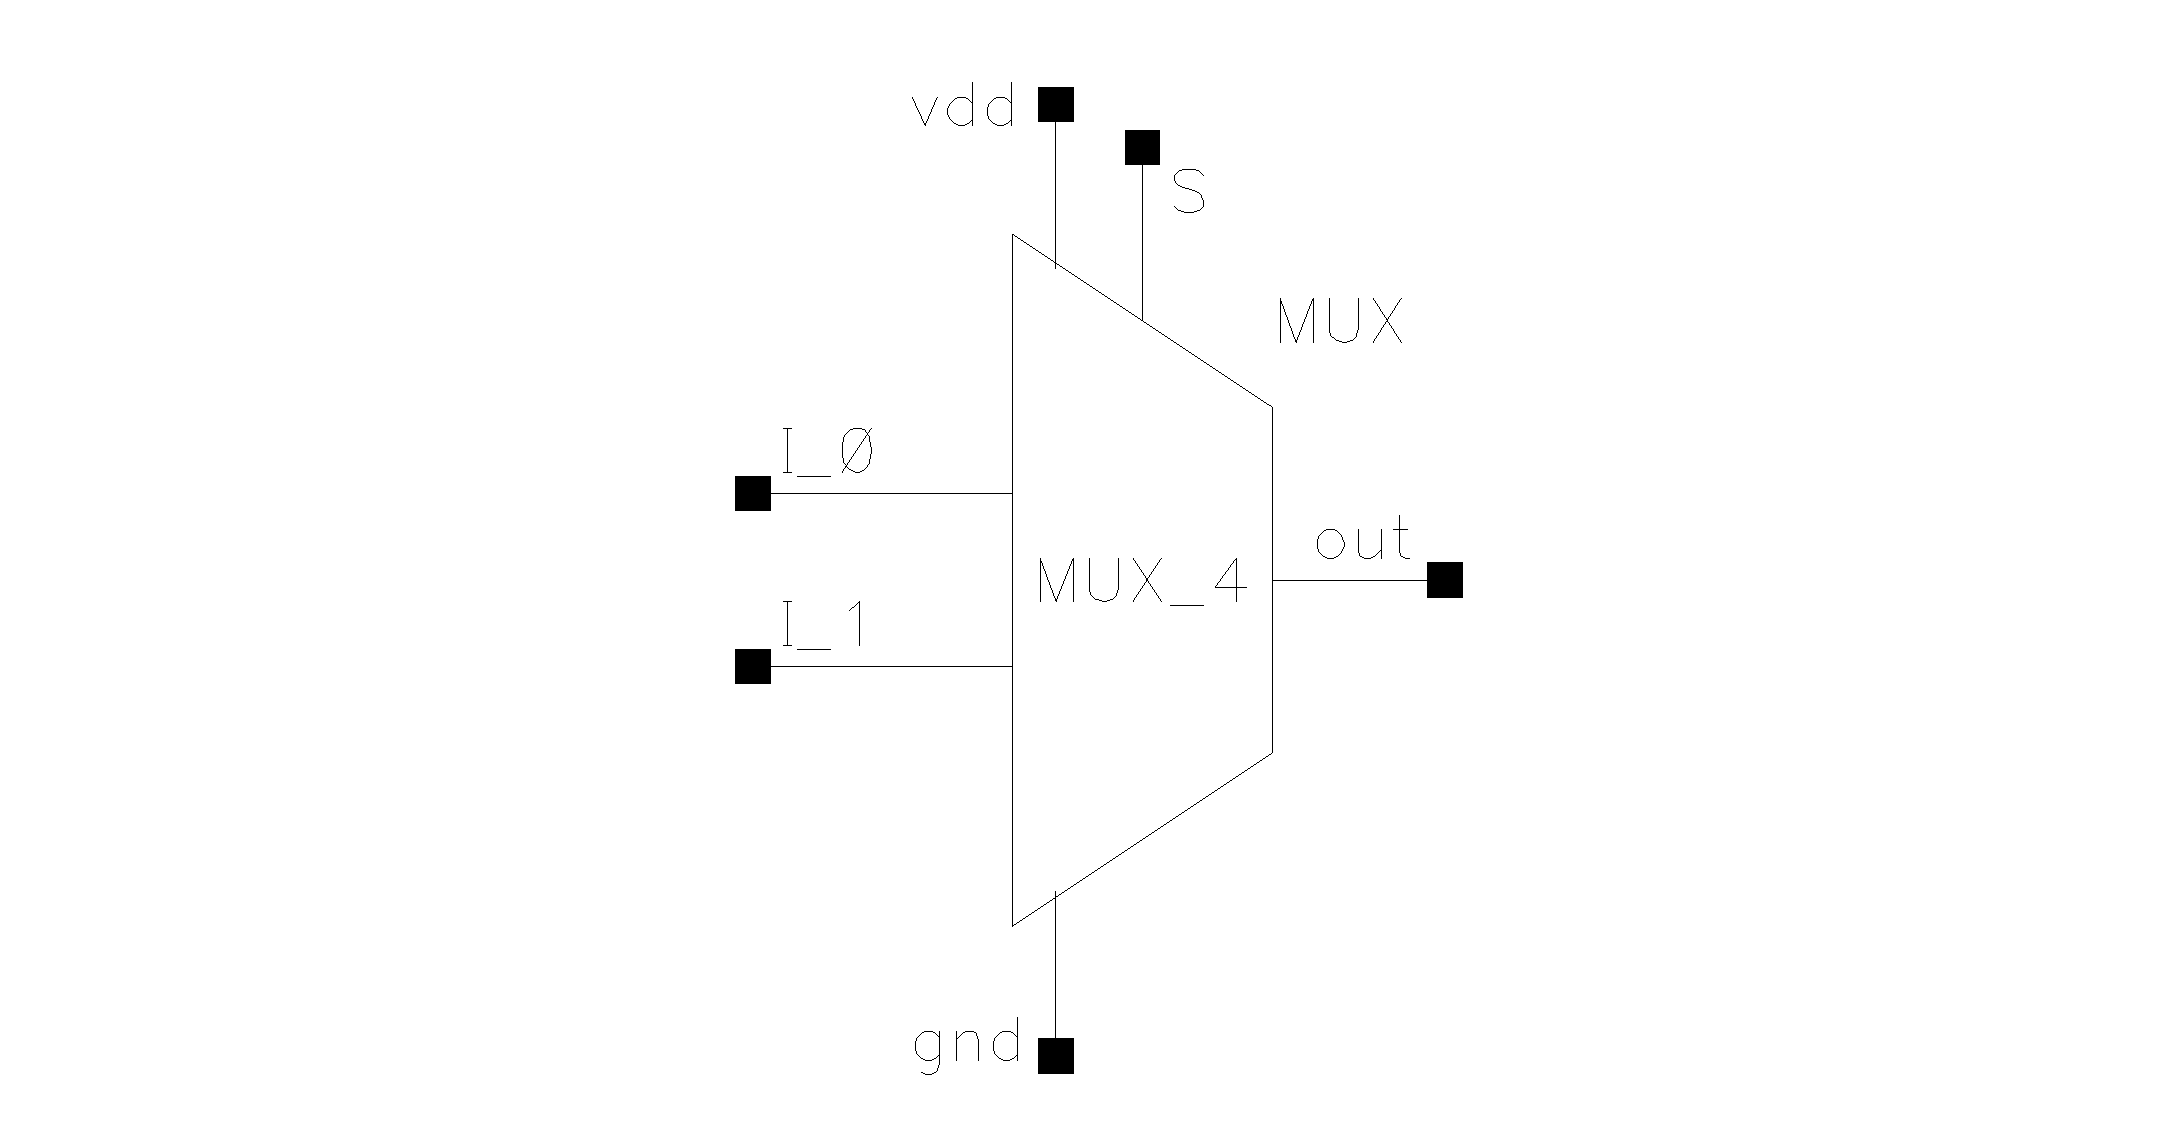
\includegraphics[width=0.5\linewidth]{writeup//figures/mux_w1_opt_sym.png}
    \caption{Enter Caption}
\end{figure}

\begin{figure}[H]
    \centering
    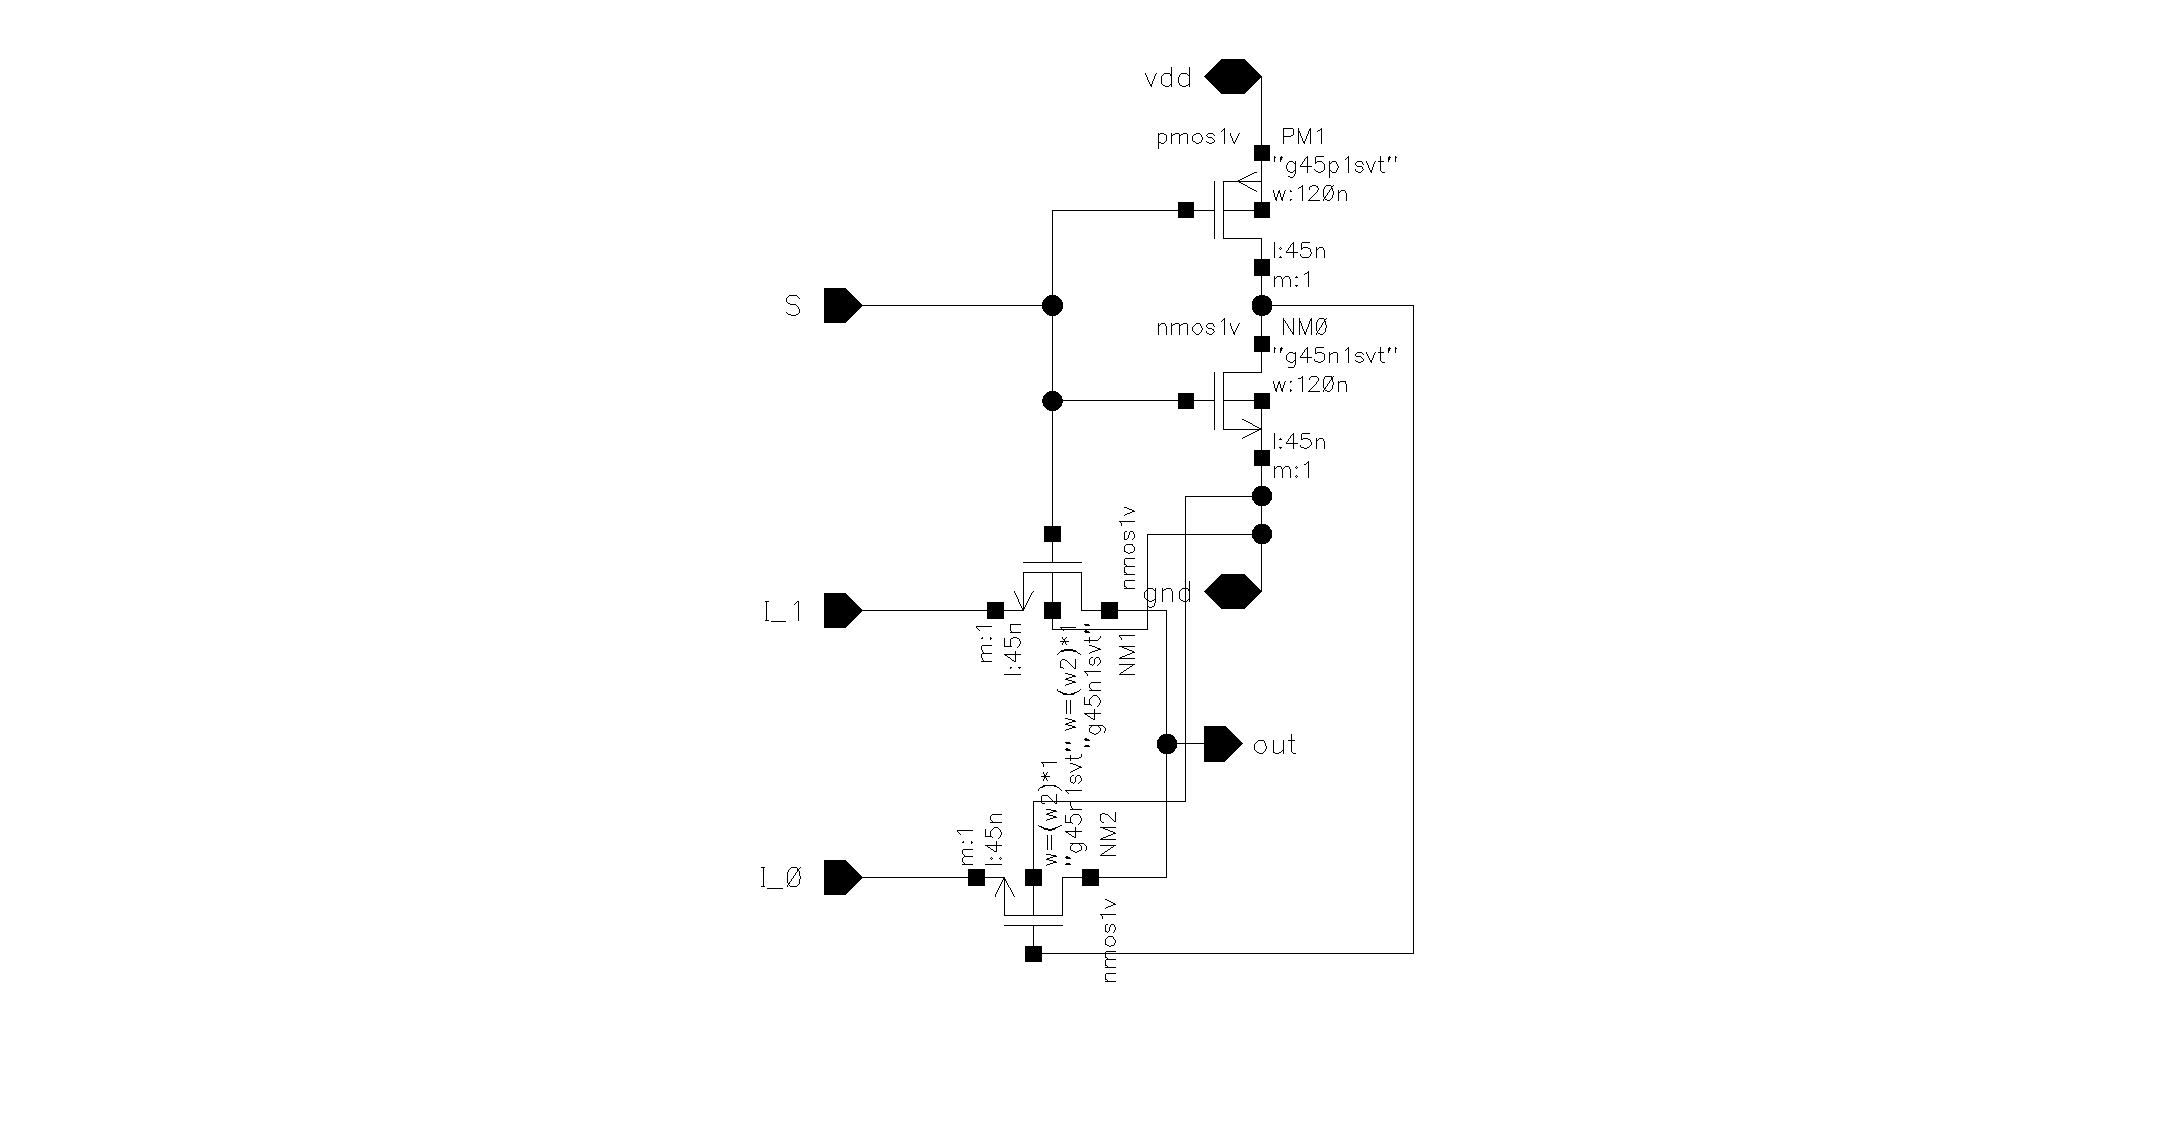
\includegraphics[width=0.5\linewidth]{writeup//figures/mux_w2_opt.png}
    \caption{Enter Caption}
\end{figure}

\begin{figure}[H]
    \centering
    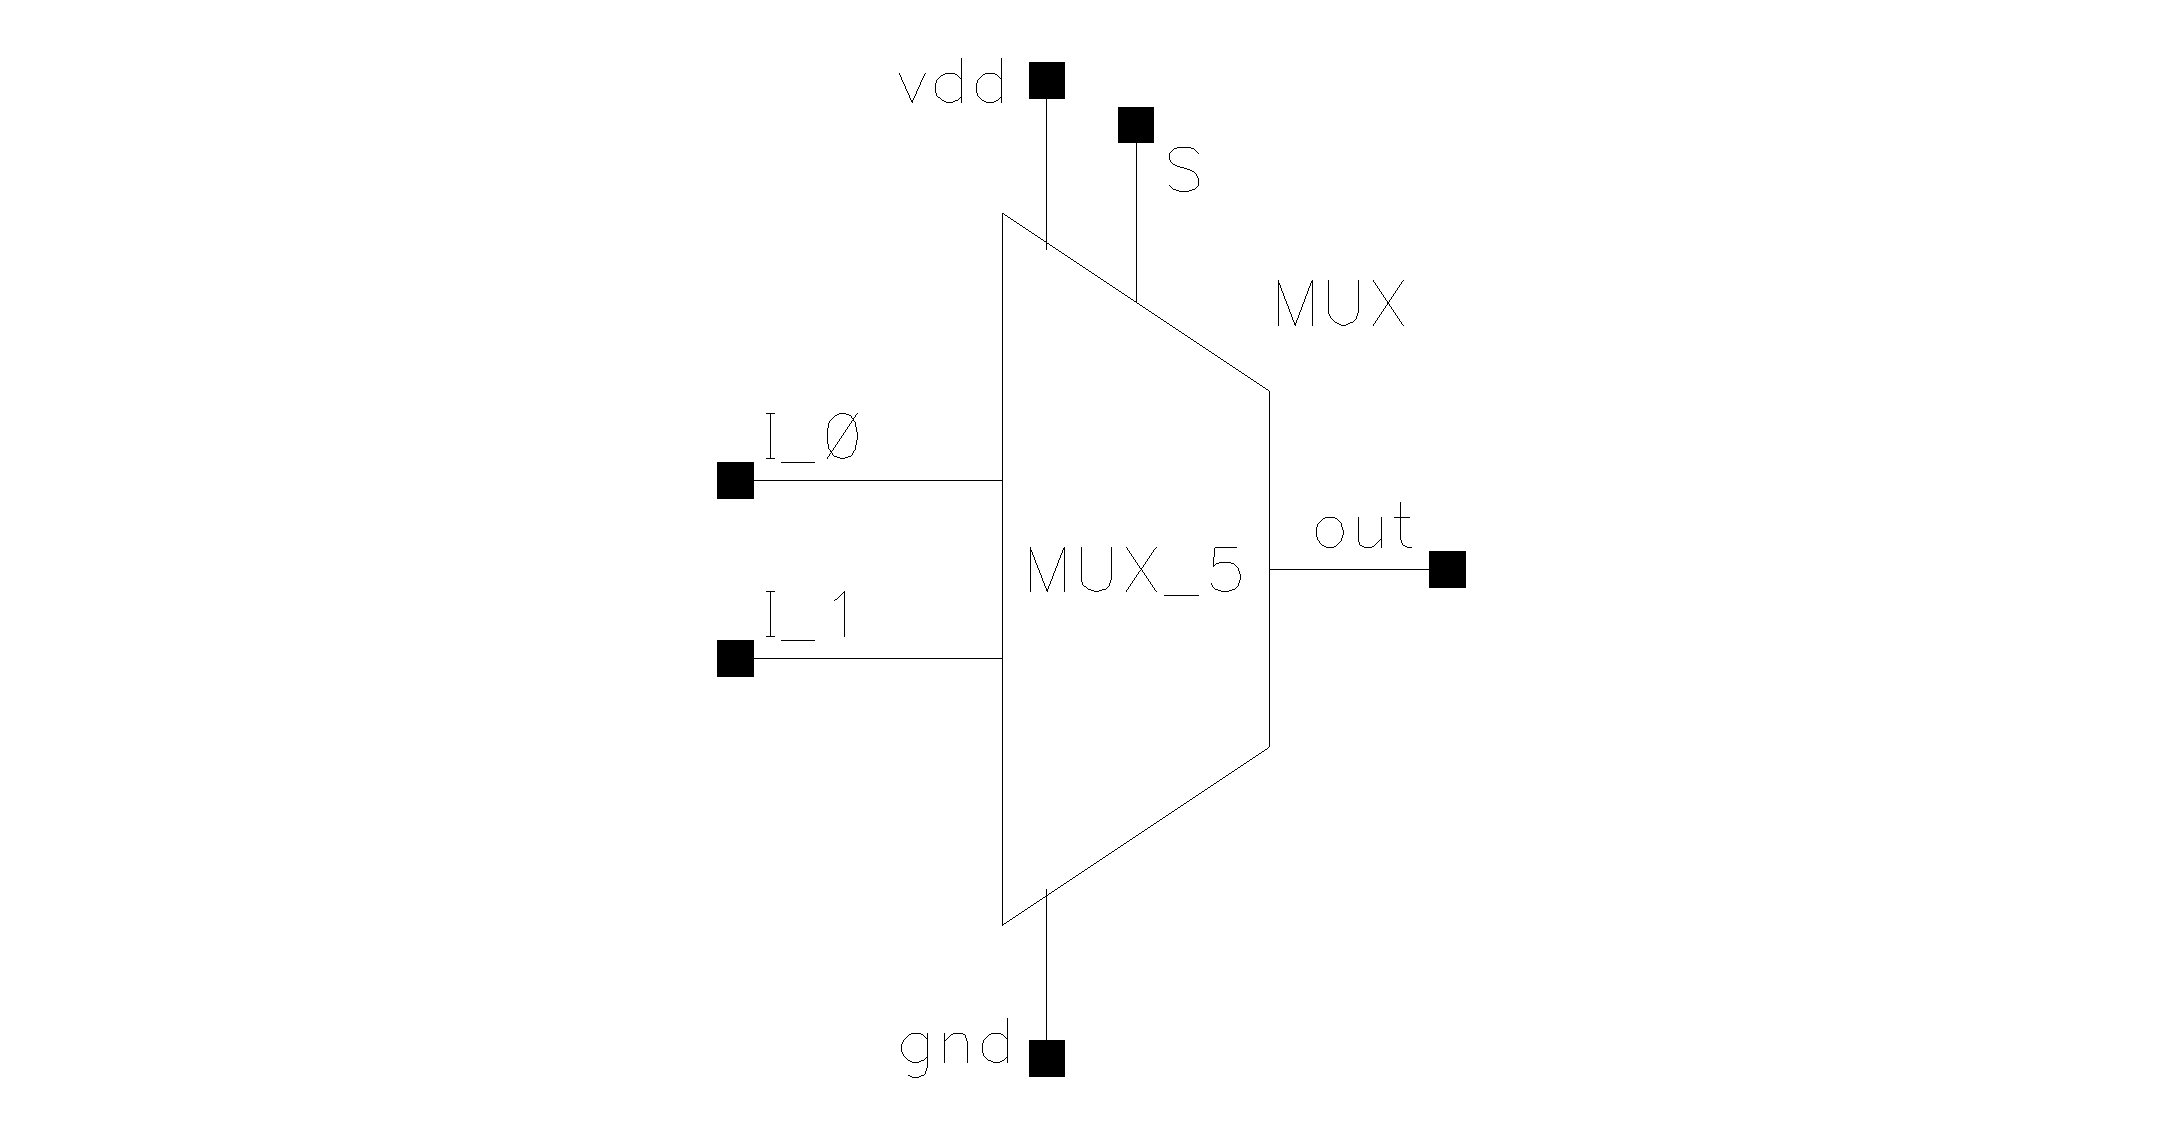
\includegraphics[width=0.5\linewidth]{writeup//figures/mux_w2_opt_sym.png}
    \caption{Enter Caption}
\end{figure}

\begin{figure}[H]
    \centering
    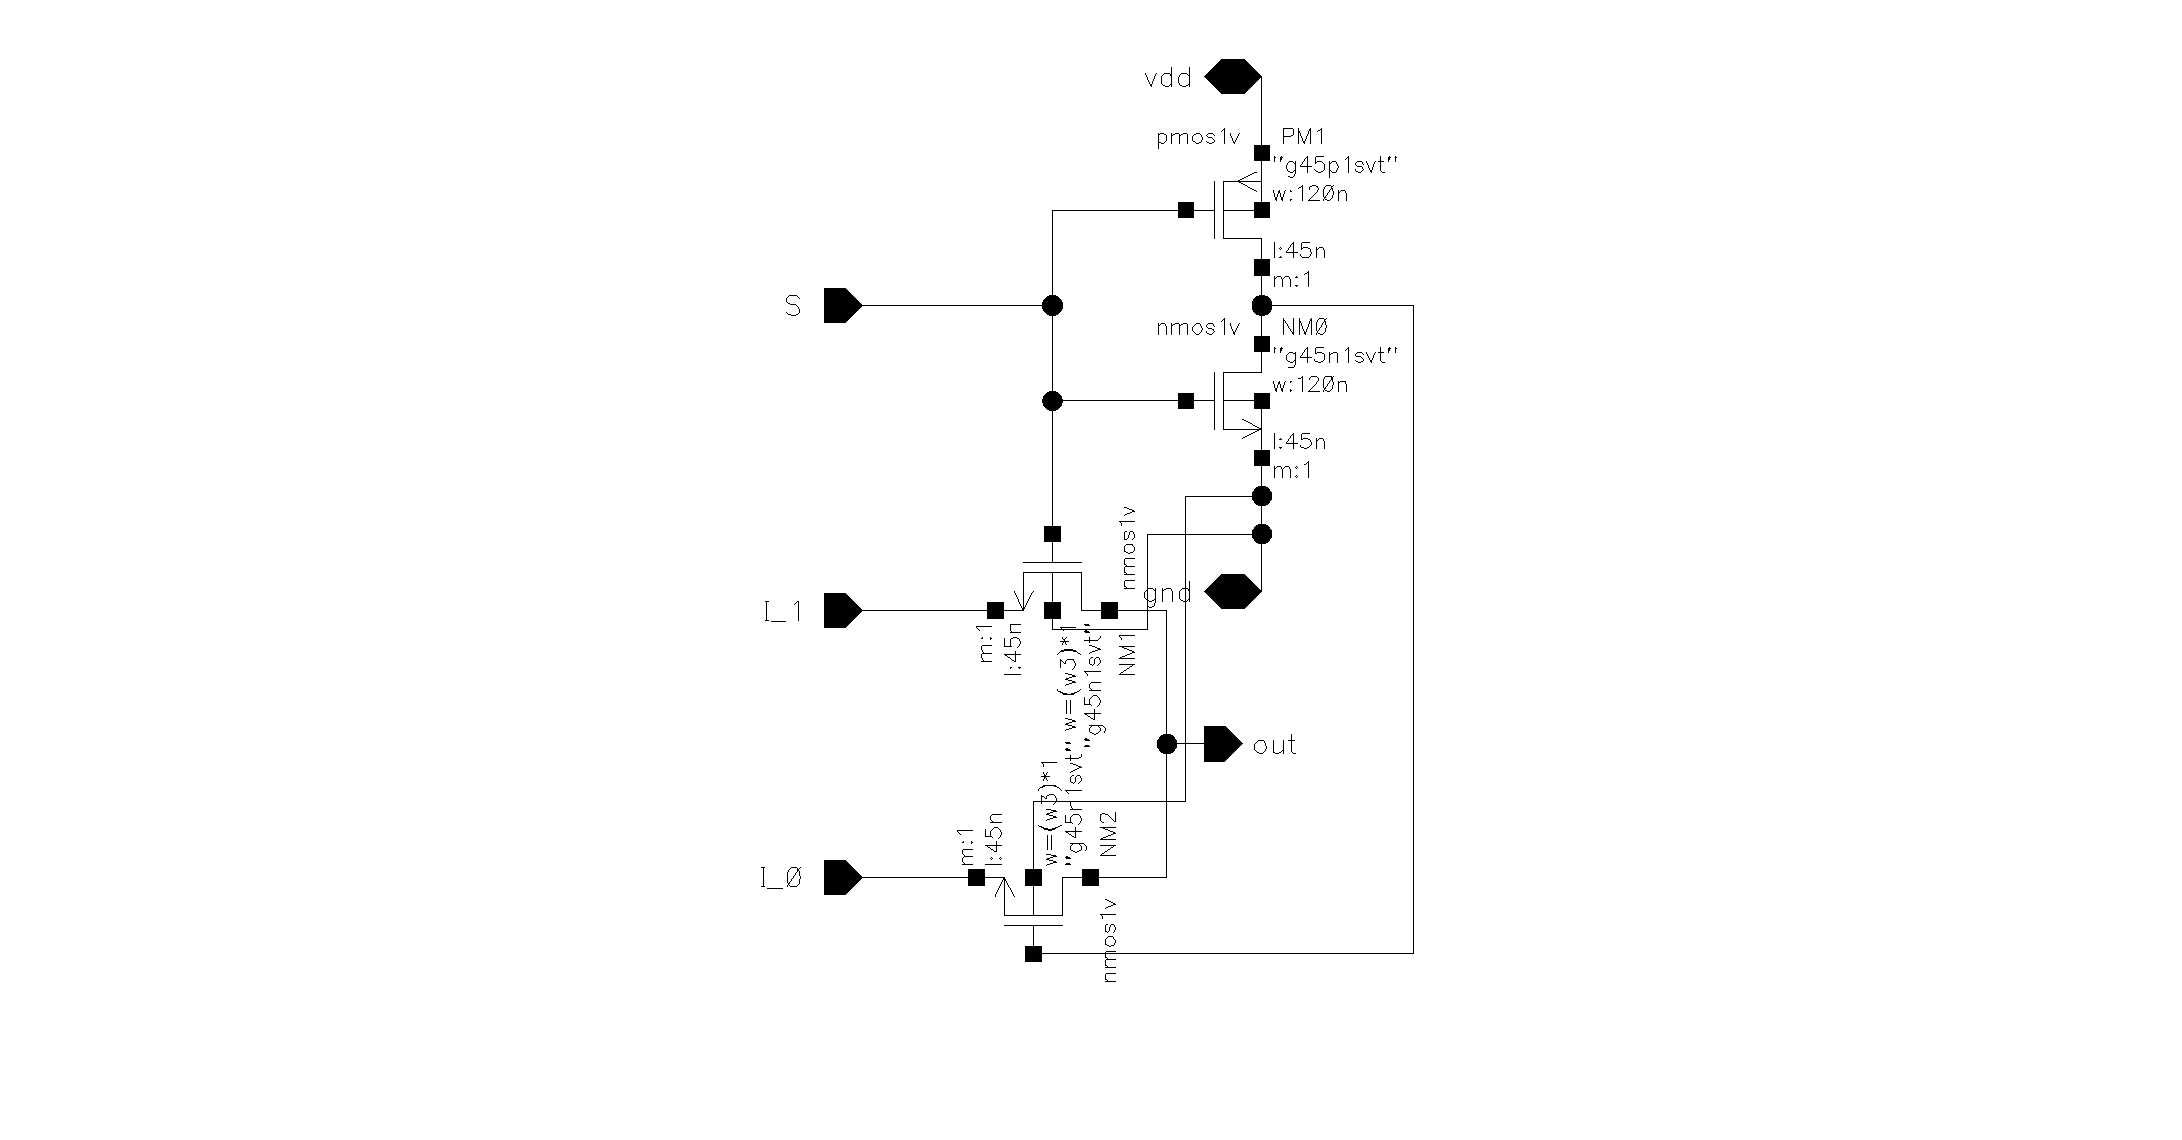
\includegraphics[width=0.5\linewidth]{writeup//figures/mux_w3_opt.png}
    \caption{Enter Caption}
\end{figure}

\begin{figure}[H]
    \centering
    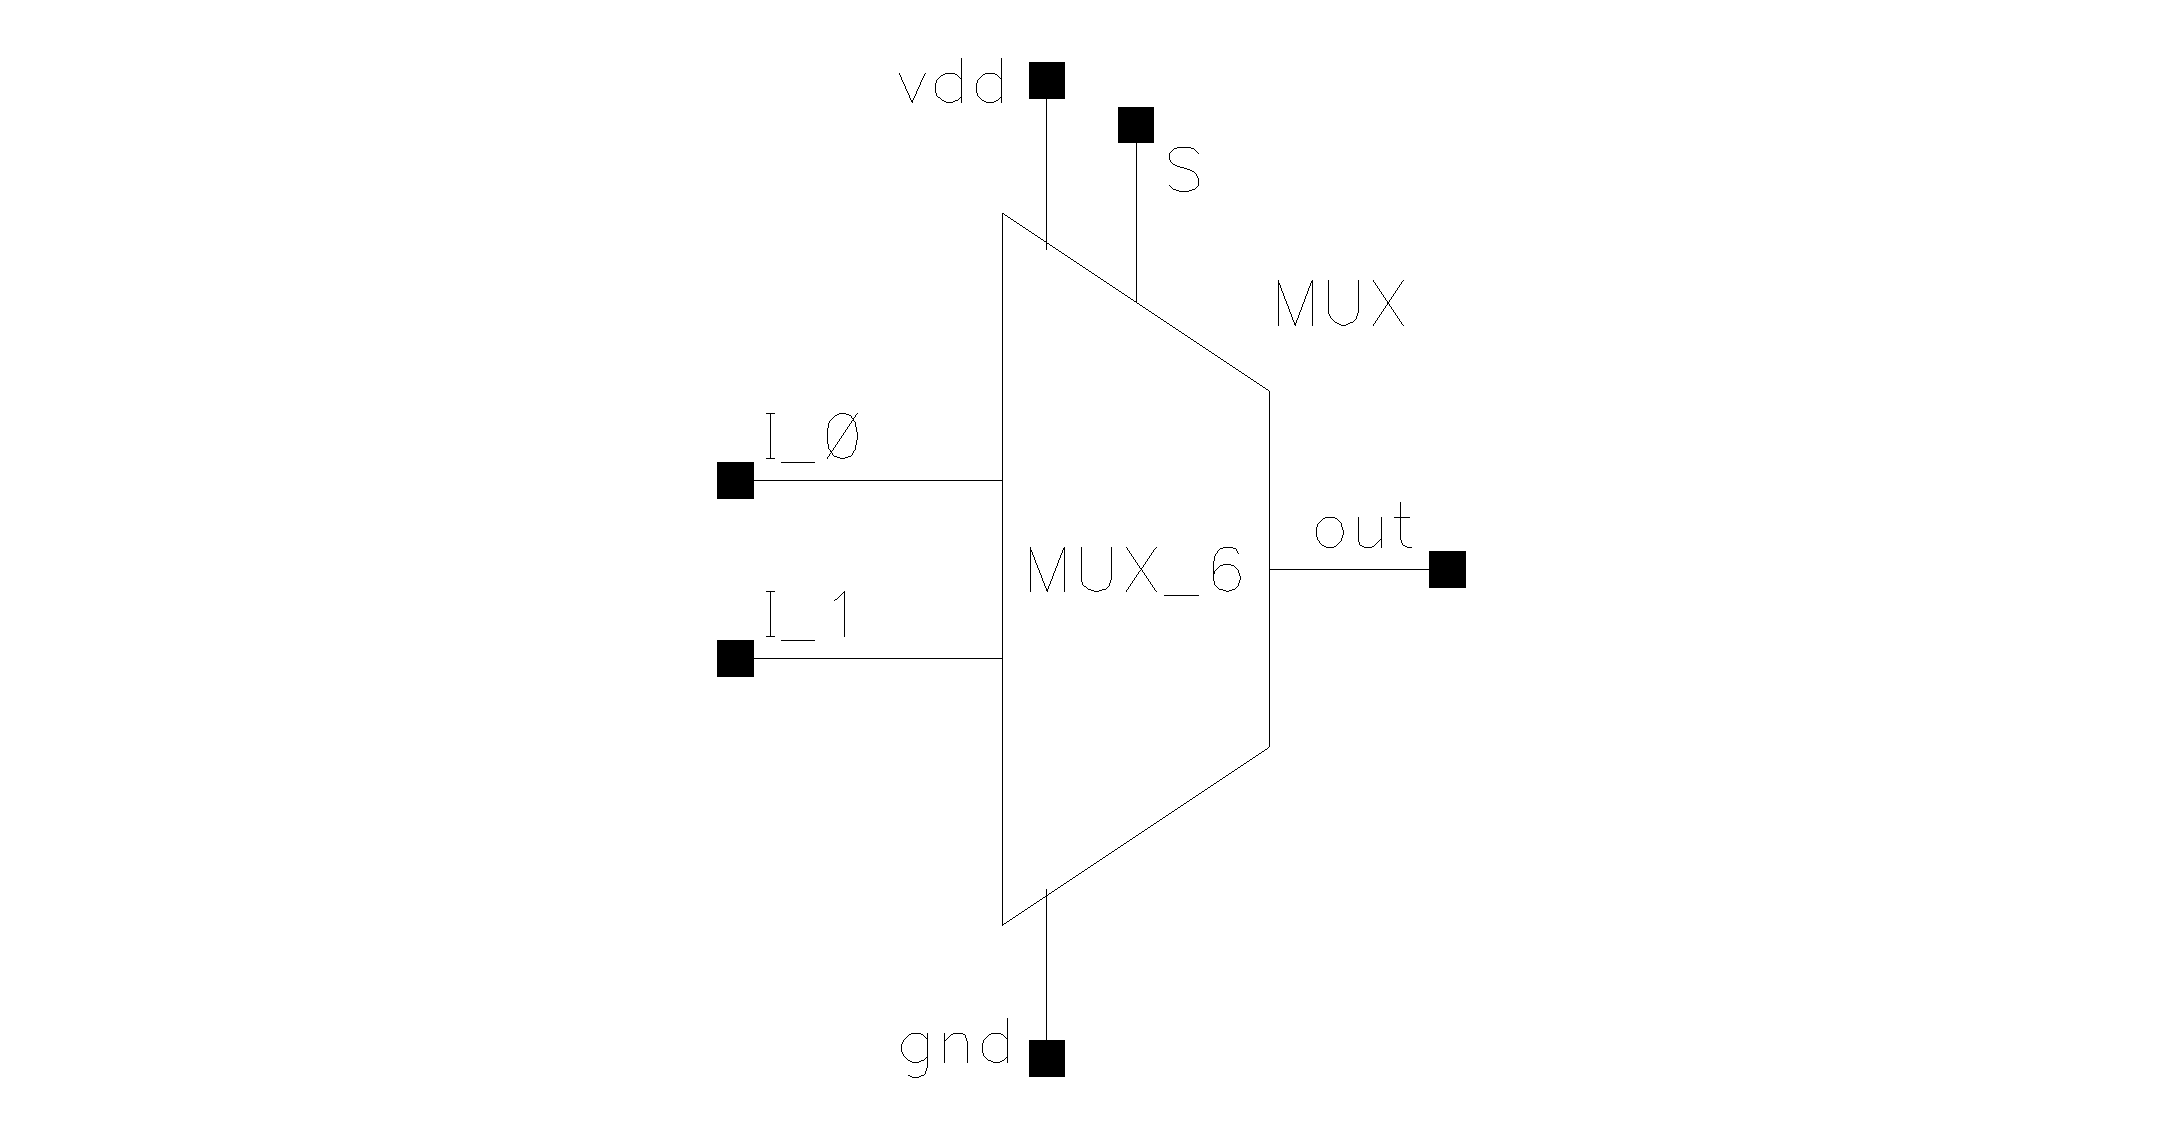
\includegraphics[width=0.5\linewidth]{writeup//figures/mux_w3_opt_sym.png}
    \caption{Enter Caption}
\end{figure}

\begin{figure}[H]
    \centering
    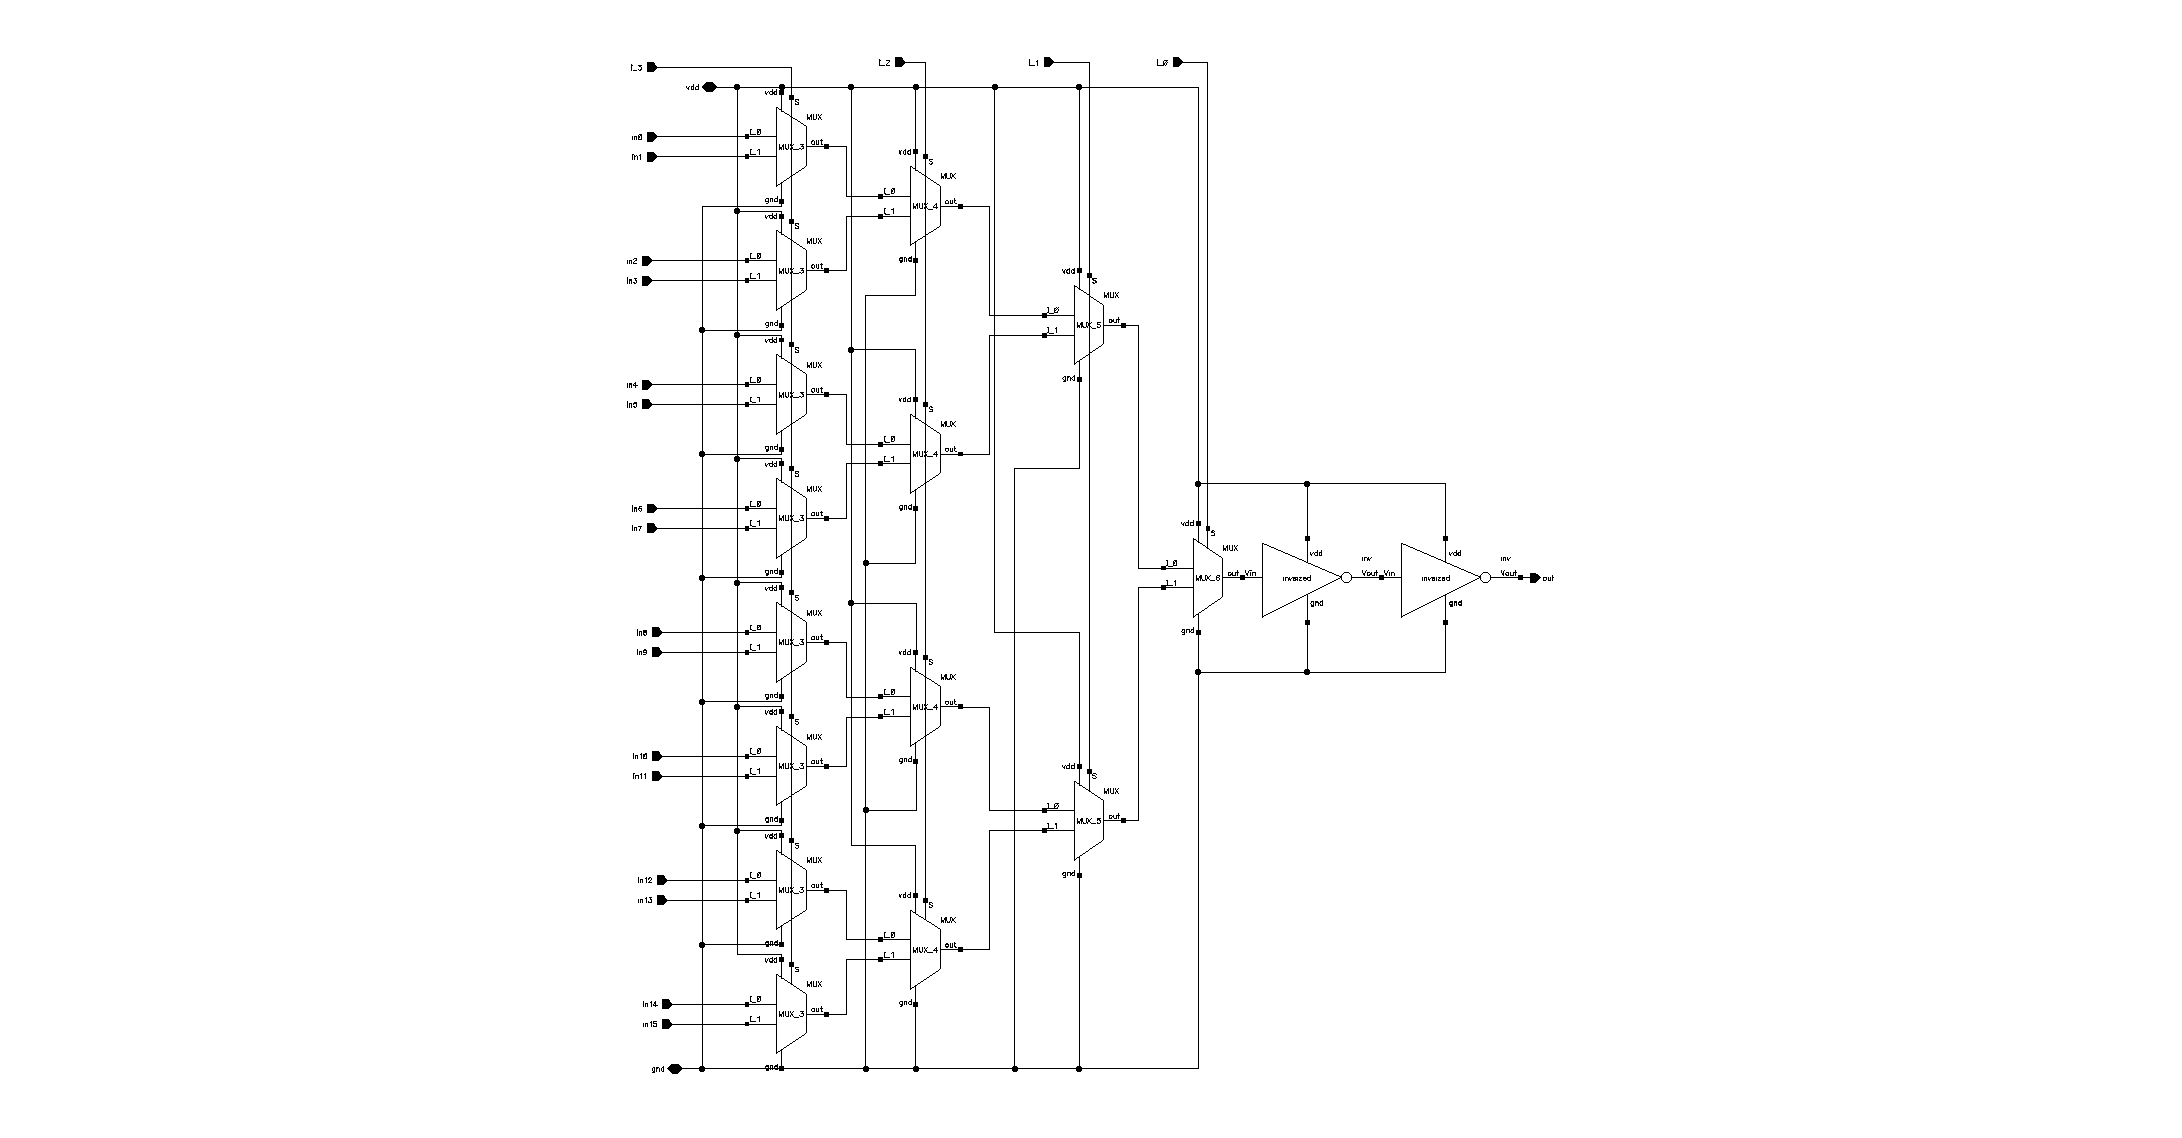
\includegraphics[width=0.5\linewidth]{writeup//figures/updated_delay_opt_LUTschem.png}
    \caption{Enter Caption}
\end{figure}

\begin{figure}[H]
    \centering
    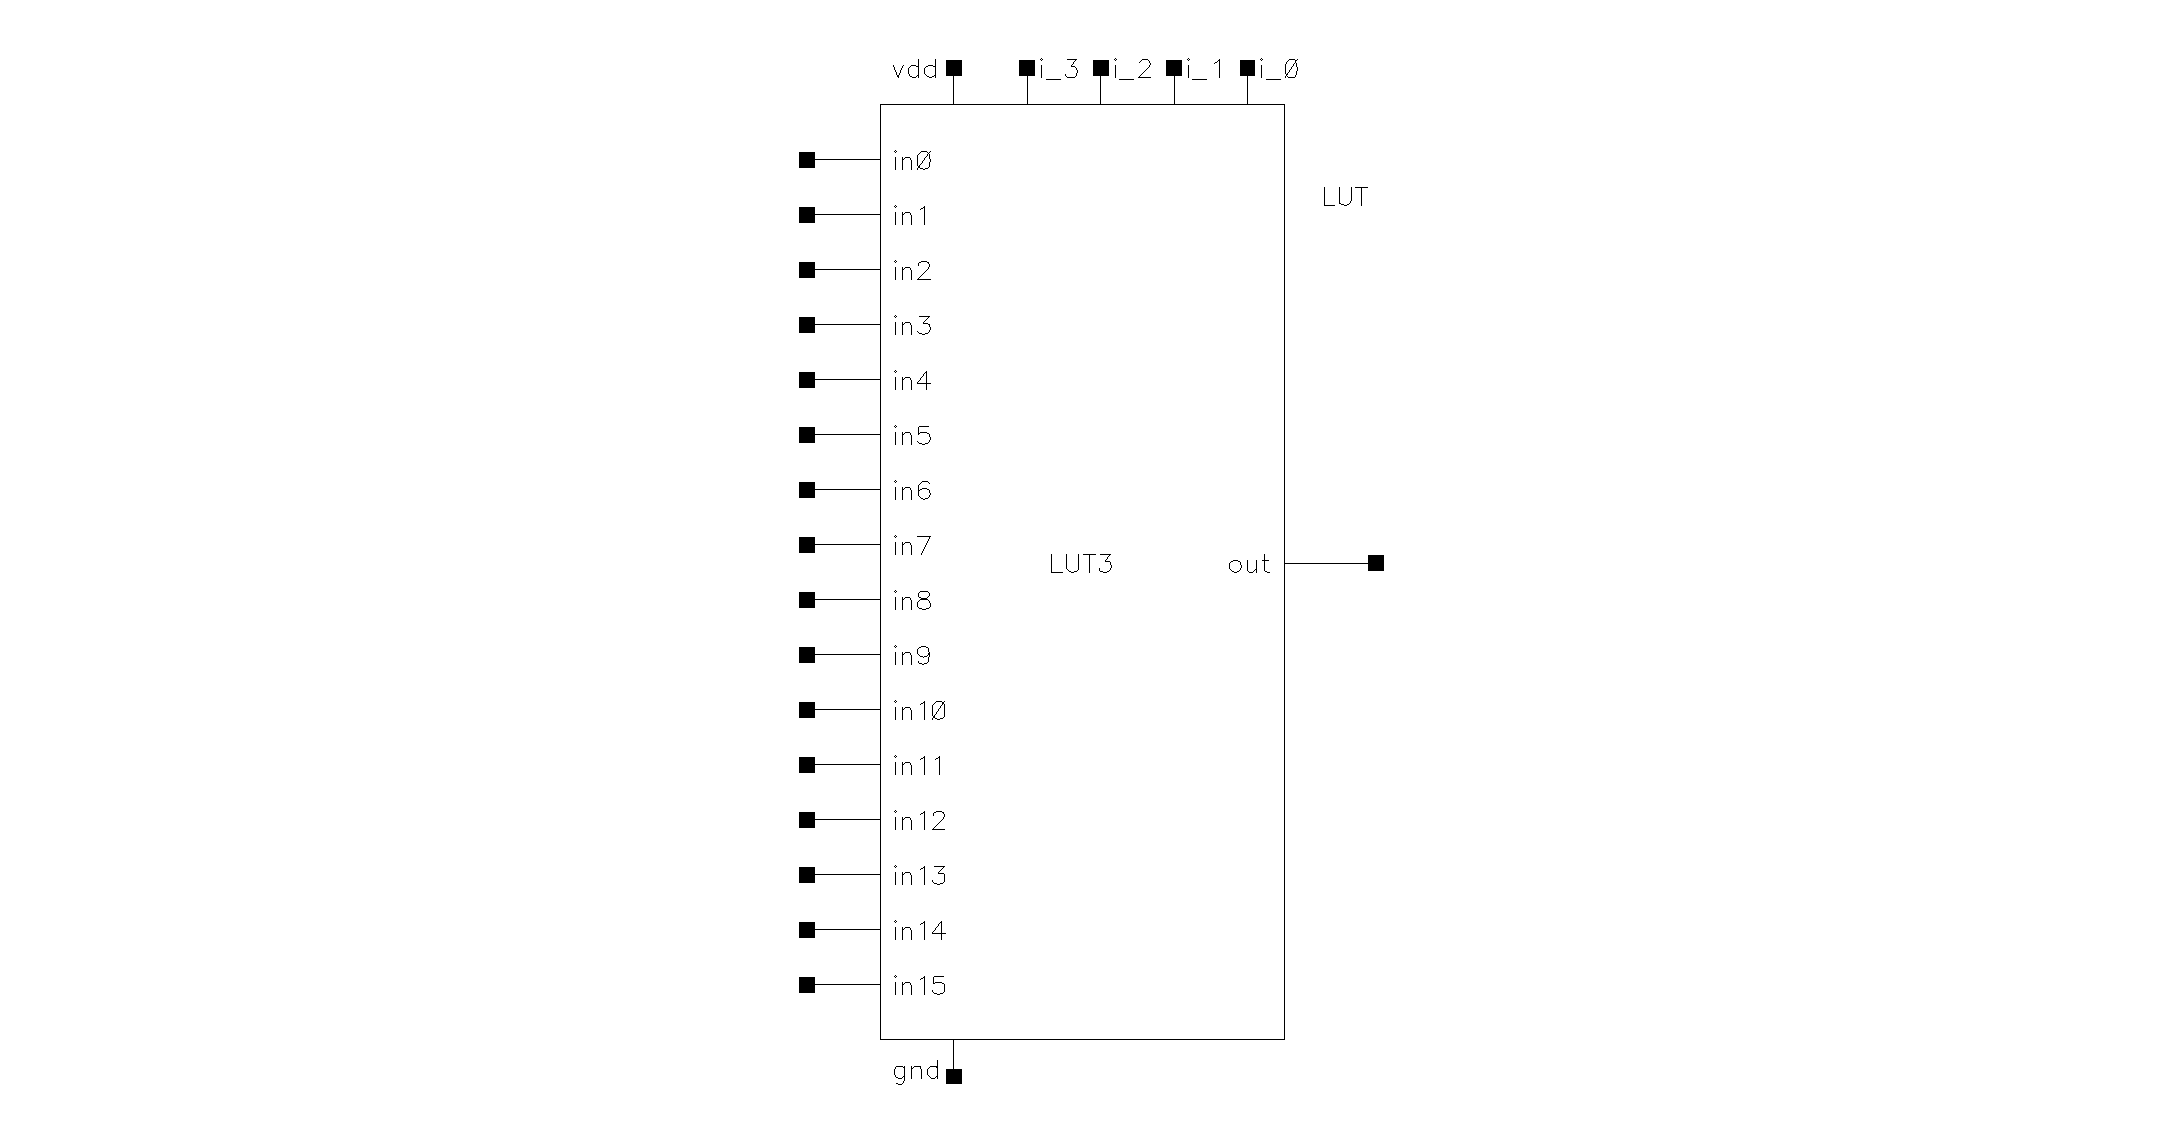
\includegraphics[width=0.5\linewidth]{writeup//figures/updated_delay_opt_LUTsym.png}
    \caption{Enter Caption}
\end{figure}


\newpage

\subsection{Optimization Process}

\begin{figure}[H]
    \centering
    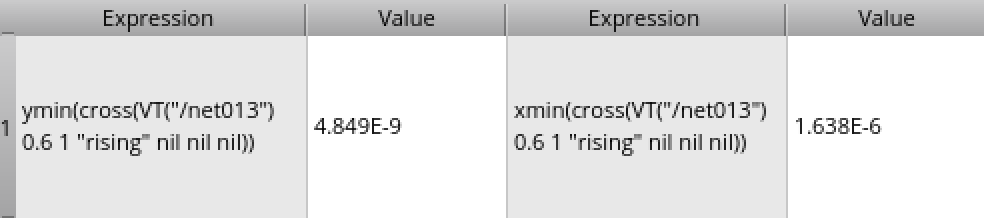
\includegraphics[width=0.5\linewidth]{writeup//figures/optimized_wmux_value.png}
    \caption{Enter Caption}
\end{figure}

\begin{figure}[H]
    \centering
    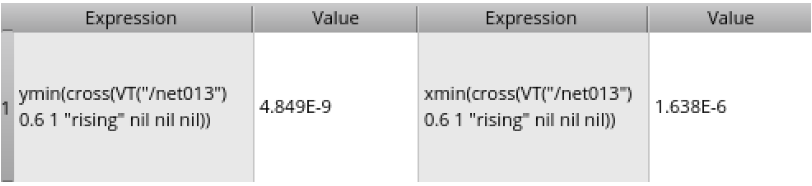
\includegraphics[width=0.5\linewidth]{writeup//figures/wmux1.png}
    \caption{Enter Caption}
\end{figure}

\begin{figure}[H]
    \centering
    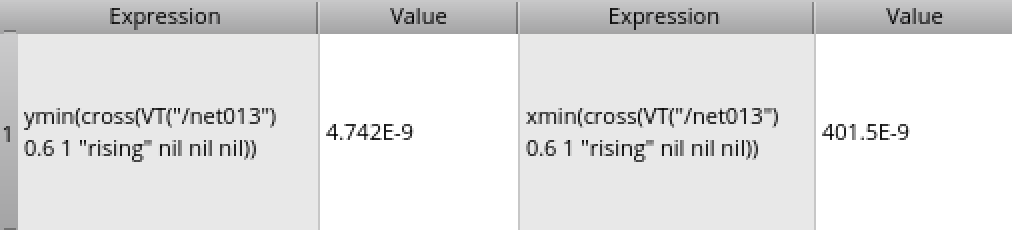
\includegraphics[width=0.5\linewidth]{writeup//figures/optimized_wbuf_value.png}
    \caption{Enter Caption}
\end{figure}

\begin{figure}[H]
    \centering
    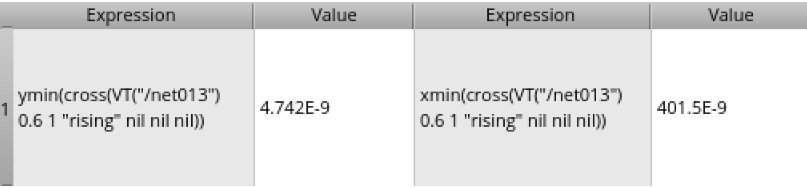
\includegraphics[width=0.5\linewidth]{writeup//figures/wbuf1.png}
    \caption{Enter Caption}
\end{figure}

\begin{figure}[H]
    \centering
    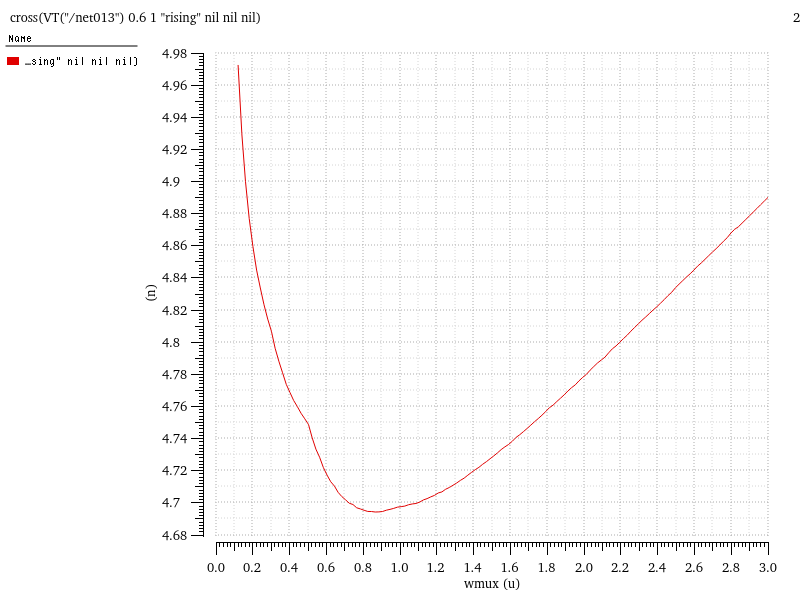
\includegraphics[width=0.5\linewidth]{writeup//figures/optimized_wmux_value2.png}
    \caption{Enter Caption}
\end{figure}

\begin{figure}[H]
    \centering
    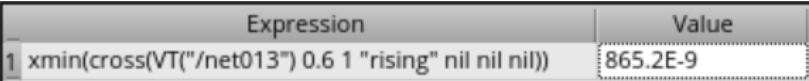
\includegraphics[width=0.5\linewidth]{writeup//figures/wmux2.png}
    \caption{Enter Caption}
\end{figure}

\begin{figure}[H]
    \centering
    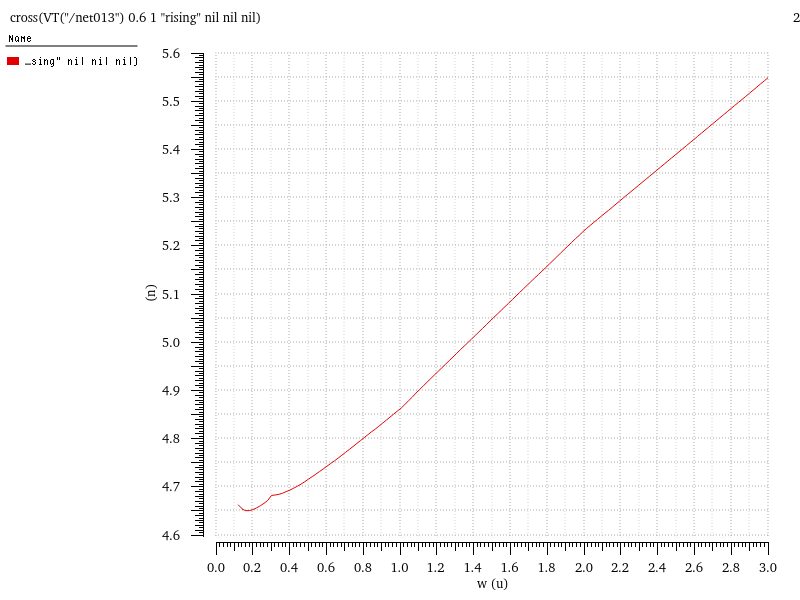
\includegraphics[width=0.5\linewidth]{writeup//figures/optimized_wbuf_value2.png}
    \caption{Enter Caption}
\end{figure}

\begin{figure}[H]
    \centering
    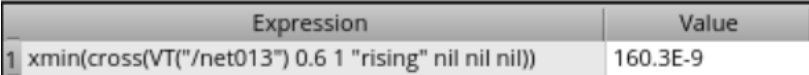
\includegraphics[width=0.5\linewidth]{writeup//figures/wbuf2.png}
    \caption{Enter Caption}
\end{figure}

\begin{figure}[H]
    \centering
    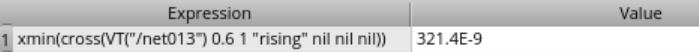
\includegraphics[width=0.5\linewidth]{writeup//figures/optimized_wmux_value_3.png}
    \caption{Enter Caption}
\end{figure}

\begin{figure}[H]
    \centering
    
\includegraphics[width=0.5\linewidth]{writeup//figures/wmux3.png}
    \caption{Enter Caption}
\end{figure}

\begin{figure}[H]
    \centering
    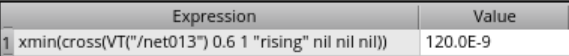
\includegraphics[width=0.5\linewidth]{writeup//figures/wbuf3.png}
    \caption{Enter Caption}
\end{figure}


\begin{figure}[H]
    \centering
    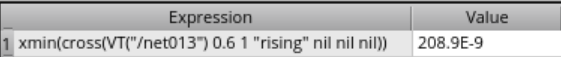
\includegraphics[width=0.5\linewidth]{writeup//figures/wmux4.png}
    \caption{Enter Caption}
\end{figure}

\begin{figure}
    \centering
    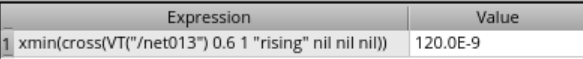
\includegraphics[width=0.5\linewidth]{writeup//figures/wbuf4.png}
    \caption{Enter Caption}
\end{figure}



\newpage

% ------------------ SECTION 7 ------------------
\section{Optimized Design Validation and Logical Test}
\subsection{Test Schematic and Case}
The muxes were designed the same way as the baseline design, but different variables were set for the widths of muxes in each stage. 



\newpage

\subsection{Simulation Results}
\subsubsection*{2:1 MUX Subcircuit Validation}
\begin{figure}[H]
    \centering
    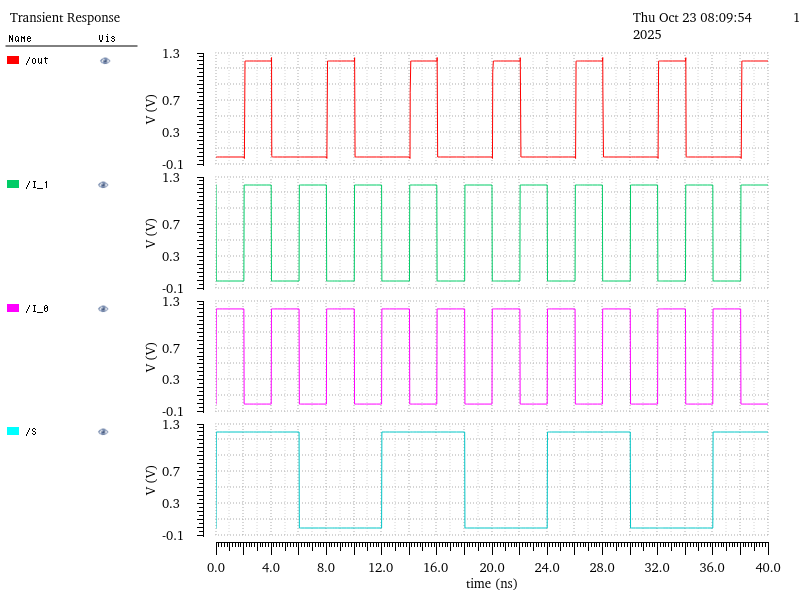
\includegraphics[width=0.5\linewidth]{writeup//figures/muxsubval.png}
    \caption{Enter Caption}
\end{figure}

The same subcircuit was used as the baseline. Widths were varied according to the stage, for optimization. In the subcircuit test, the select input \( S \) is toggled while \( I_0 \) and \( I_1 \) run as independent square waves. 
Whenever \( S \) is high, the output waveform overlays \( I_1 \) with only a small propagation delay; whenever \( S \) is low, the output overlays \( I_0 \). 
Each handoff can be observed at the transitions of \( S \): during every \( S=1 \) interval the output \( V_{\text{out}} \) matches \( I_1 \), and during every \( S=0 \) interval it matches \( I_0 \). 
This behavior corresponds to the expected logic equation 
\[
V_{\text{out}} = S \cdot I_1 + \overline{S} \cdot I_0
\]
for a 2:1 pass-gate multiplexer. 
The simulation therefore verifies that the subcircuit operates correctly.

\subsubsection*{16:1 LUT Validation}
\begin{figure}[H]
    \centering
    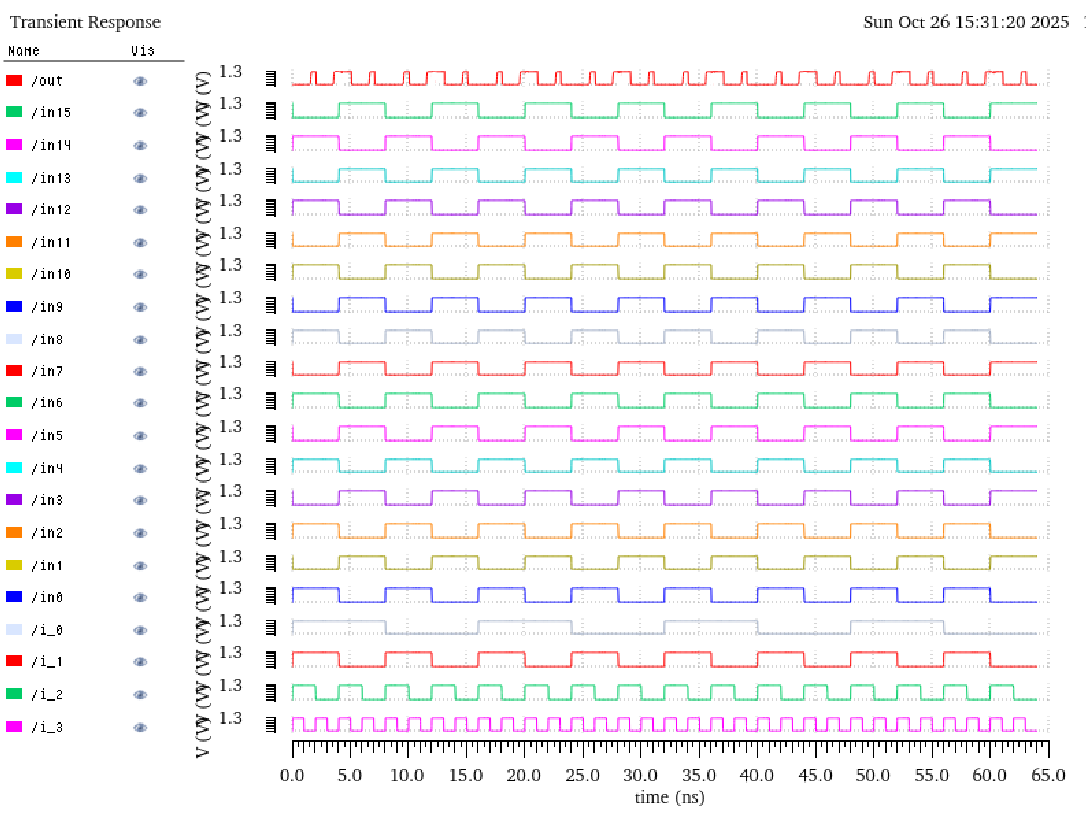
\includegraphics[width=0.5\linewidth]{writeup//figures/lut_opt_validation_sim_updated.png}
    \caption{Enter Caption}
\end{figure}
The overall test schematic was the same for optimized compared to baseline, except the widths changed for each stage, based on a parametric sweep. After inputting the widths found from the sweep (see optimized delay measurement section), the following validation results were obtained.  For the full 16:1 LUT, all sixteen input combinations (\(2^4\)) were simulated by varying the four address lines from \(0000\) through \(1111\). 
In each address state, the output \(V_{\text{out}}\) aligns with exactly one corresponding data input. 
Specifically, when the address equals \(0000\), \(\text{IN}_0\) propagates to the output; as the address increments, \(\text{IN}_1, \text{IN}_2, \ldots, \text{IN}_{15}\) sequentially drive the output. 
Rising and falling edges on \(V_{\text{out}}\) coincide precisely with the selected input, while nonselected inputs show no coupling. 
Because all address combinations were verified and the output correctly reflected the selected data input each time, the 16:1 LUT simulation confirms correct functionality.

\newpage
% ------------------ SECTION 8 ------------------
\section{Optimized Delay Measurement}
\subsubsection{Test Schematic}
\begin{figure}[H]
    \centering
    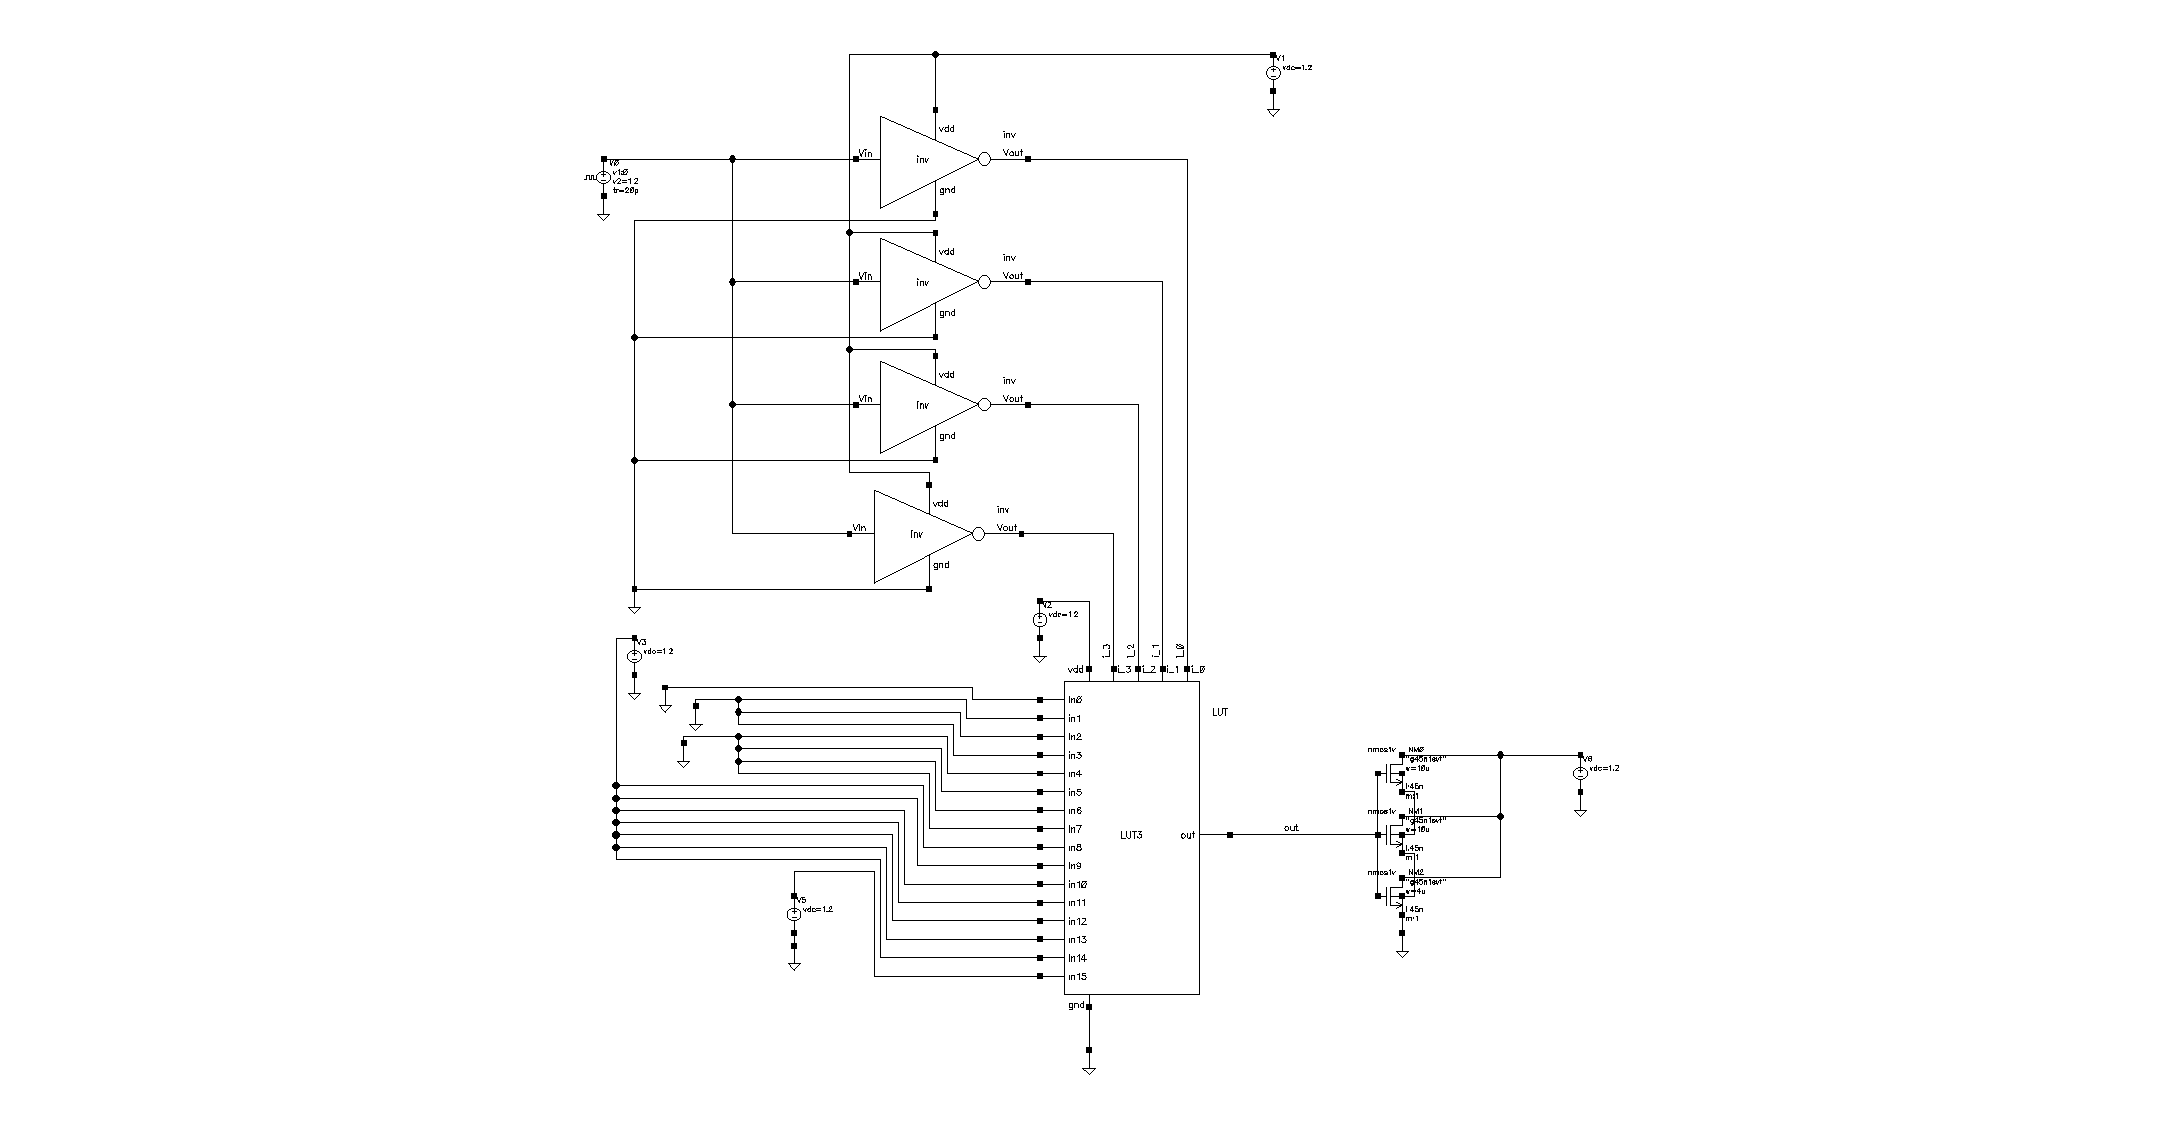
\includegraphics[width=0.5\linewidth]{writeup//figures/updated_delay_opt_testschem.png}
    \caption{Enter Caption}
\end{figure}

\newpage

\begin{figure}[H]
    \centering
    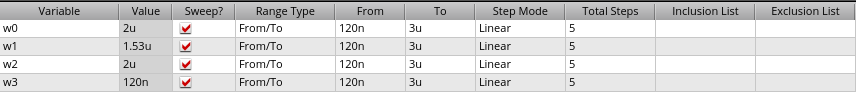
\includegraphics[width=0.5\linewidth]{writeup//figures/wmux_all_parametric_sweep_setup.png}
    \caption{Enter Caption}
\end{figure}

\begin{figure}[H]
    \centering
    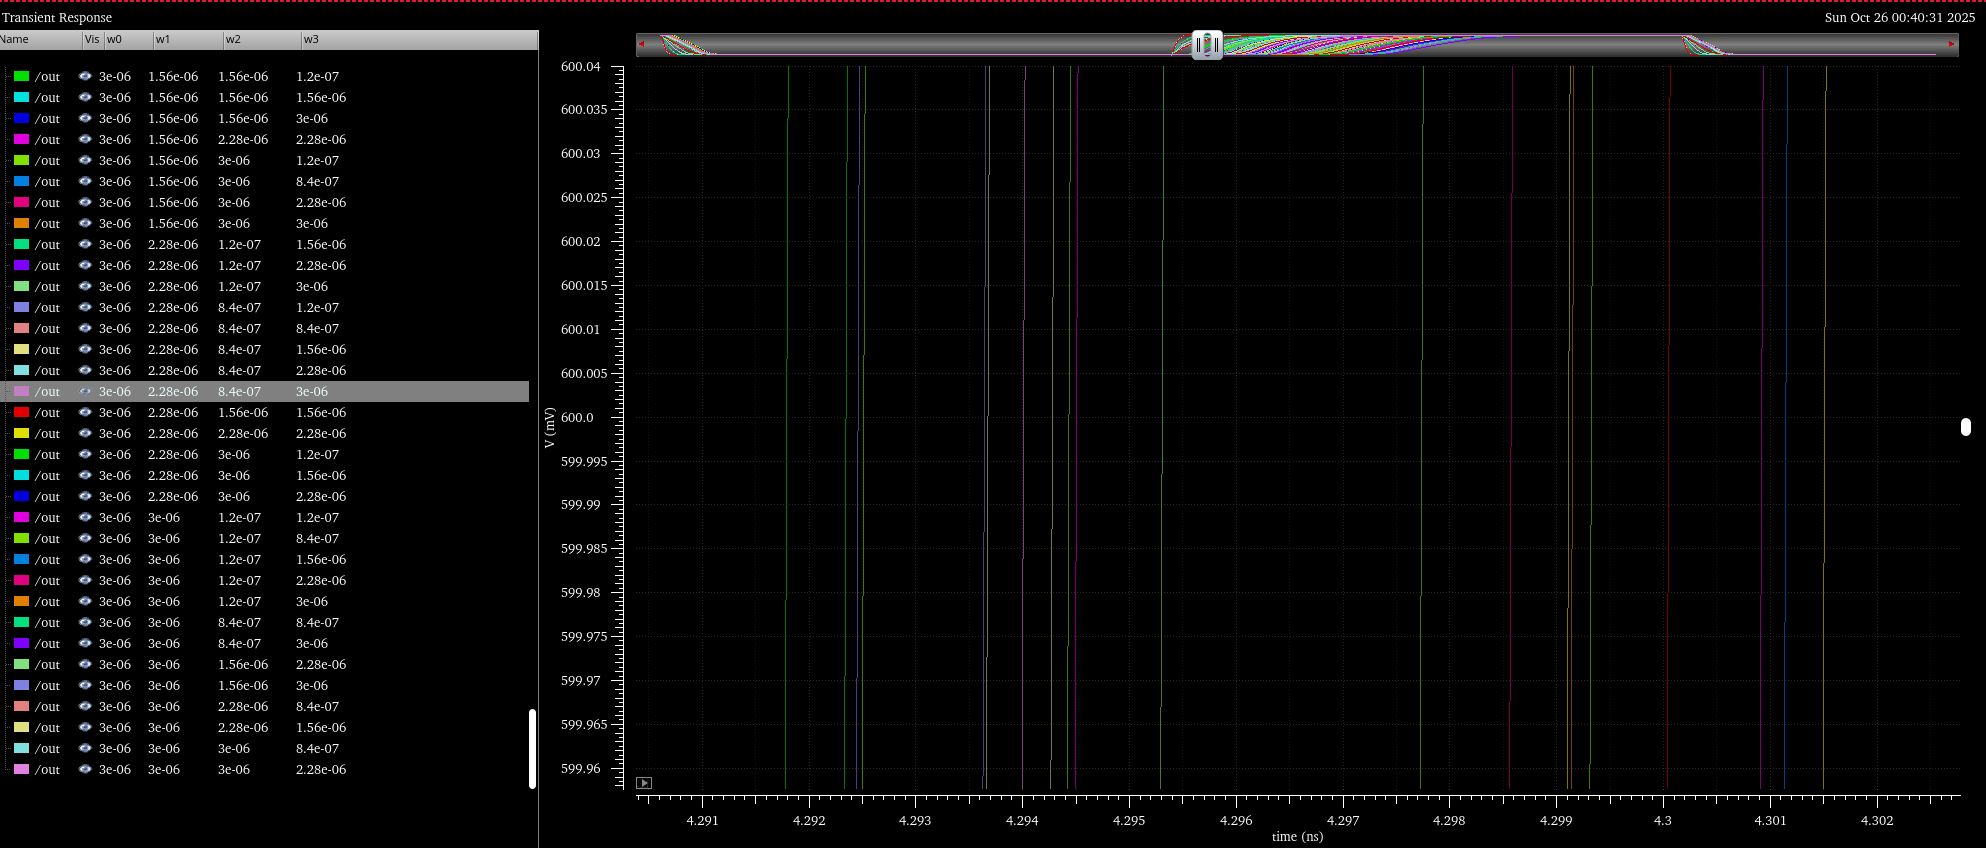
\includegraphics[width=\linewidth]{writeup//figures/wmux_all_zoomed_parametrics_weep2.png}
    \caption{Enter Caption}
\end{figure}

\begin{figure}
    \centering
    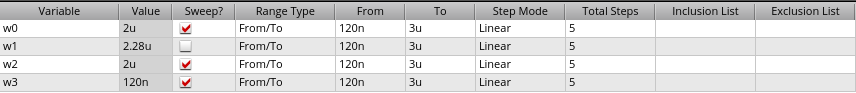
\includegraphics[width=1\linewidth]{writeup//figures/wmux_3_parametric_sweep_setup.png}
    \caption{Enter Caption}
\end{figure}

\begin{figure}[H]
    \centering
    \includegraphics[width=0.5\linewidth]{writeup//figures/wmux_3_parametrics_weep.png}
    \caption{Enter Caption}
\end{figure}

\begin{figure}[H]
    \centering
    \includegraphics[width=0.5\linewidth]{writeup//figures/wmux_2_parametric_sweep_setup.png}
    \caption{Enter Caption}
\end{figure}

\begin{figure}[H]
    \centering
    \includegraphics[width=0.5\linewidth]{writeup//figures/wmux_2_parametrics_weep.png}
    \caption{Enter Caption}
\end{figure}

\begin{figure}[H]
    \centering
    \includegraphics[width=0.5\linewidth]{writeup//figures/wmux_1_parametric_sweep_setup.png}
    \caption{Enter Caption}
\end{figure}

\begin{figure}[H]
    \centering
    \includegraphics[width=0.5\linewidth]{writeup//figures/wmux_1_parametrics_weep.png}
    \caption{Enter Caption}
\end{figure}


\begin{figure}[H]
    \centering
    \includegraphics[width=0.5\linewidth]{writeup//figures/wmux_1_parametric_sweep_setup.png}
    \caption{Enter Caption}
\end{figure}




\newpage

\subsection{Simulation Results and Metric Value}

\begin{figure}[H]
    \centering
    \includegraphics[width=\linewidth]{writeup//figures/optimized_delay_ADEL_setup.png}
    \caption{Enter Caption}
\end{figure}

\begin{figure}[H]
    \centering
    \includegraphics[width=0.5\linewidth]{writeup//figures/updated_delay_opt.png}
    \caption{Enter Caption}
\end{figure}
From the transient response, the measured $50\%$ crossing times are
\[
t_{\text{in},50\%\downarrow} = 4.119~\text{ns}, \quad
t_{\text{out},50\%\uparrow} = 4.272~\text{ns}, \quad
t_{\text{in},50\%\uparrow} = 8.115~\text{ns}, \quad
t_{\text{out},50\%\downarrow} = 8.196~\text{ns}.
\]
The propagation delays are therefore
\[
t_{PLH} = t_{\text{out},50\%\uparrow} - t_{\text{in},50\%\downarrow}
        = 4.272~\text{ns} - 4.119~\text{ns}
        = \boxed{0.153~\text{ns}},
\]
\[
t_{PHL} = t_{\text{out},50\%\downarrow} - t_{\text{in},50\%\uparrow}
        = 8.196~\text{ns} - 8.115~\text{ns}
        = \boxed{0.081~\text{ns}}.
\]
The average propagation delay is
\[
t_P = \frac{t_{PLH} + t_{PHL}}{2}
     = \frac{0.153 + 0.081}{2}
     = \boxed{0.117~\text{ns}}.
\]
The percentage deviation of each transition from the average is
\[
\frac{t_{PLH} - t_P}{t_P} \times 100 = \boxed{+30.8\%}, 
\qquad
\frac{t_{PHL} - t_P}{t_P} \times 100 = \boxed{-30.8\%}.
\]
Comparing against the baseline LUT delay of $t_{P,\text{baseline}} = 0.8275~\text{ns}$, the delay-optimized LUT exhibits a significant improvement:
\[
\text{Speedup} 
= \frac{t_{P,\text{baseline}} - t_P}{t_{P,\text{baseline}}} \times 100
= \frac{0.8275 - 0.117}{0.8275} \times 100
= \boxed{85.9\%~\text{faster}}.
\]
Hence, the optimized LUT demonstrates nearly an order of magnitude reduction in propagation delay, indicating a substantial timing enhancement while maintaining consistent rise–fall symmetry.





\newpage

% ------------------ SECTION 9 ------------------
\section{Optimized Frequency Measurement}
\subsection{Test Schematic}



\newpage

\subsection{Simulation Results and Metric Value}

\begin{figure}[H]
    \centering
    \includegraphics[width=0.5\linewidth]{writeup//figures/max_frequencies_optimized.png}
    \caption{Enter Caption}
\end{figure}



\newpage

% ------------------ SECTION 10 ------------------
\section{Optimized Energy Measurement}
\subsection{Test Schematic}

\begin{figure}[H]
    \centering
    \includegraphics[width=0.5\linewidth]{writeup//figures/updated_energy_opt_testchem.png}
    \caption{Enter Caption}
\end{figure}


\newpage

\subsection{Test Case}



\newpage

\subsection{Simulation Results and Metric Value}

\begin{figure}
    \centering
    \includegraphics[width=0.5\linewidth]{writeup//figures/optimized_energy_val.png}
    \caption{Enter Caption}
\end{figure}
\newpage

% ------------------ SECTION 11 ------------------
\section{Comparison Table}



\newpage

% ------------------ SECTION 12 ------------------
\section{Discussion and Conclusions}



\end{document}